%\documentclass[conference,a4paper,10pt,oneside,final]{tp}
\documentclass[10pt]{book}
\usepackage[utf8]{inputenc}   	% caracteres especiales (acentos, eñes)
\usepackage{mylatex} 			% mi paquete de características LaTeX

  
%------------------------------------------------------------------------------------------------------------------------------------------
%	ENCABEZADO Y PIE DE PÁGINA
%------------------------------------------------------------------------------------------------------------------------------------------
\pagestyle{fancy}
\fancyhf{}
\lhead{Sistemas Operativos}
\chead{Año 2016}
\rhead{Resumen}
\headsep = 1.5 cm
\lfoot{Gentile - Rosales - Santellán}
\cfoot{SO - Resumen}
\rfoot{\thepage}

%------------------------------------------------------------------------------------------------------------------------------------------
%	AJUSTES INICIALES
%------------------------------------------------------------------------------------------------------------------------------------------


%------------------------------------------------------------------------------------------------------------------------------------------
%	INICIO DEL DOCUMENTO
%------------------------------------------------------------------------------------------------------------------------------------------
\begin{document}

%------------------------------------------------------------------------------------------------------------------------------------------
%	COMIENZO DE CARÁTULA
%------------------------------------------------------------------------------------------------------------------------------------------
\begin{titlepage}
\newcommand{\HRule}{\rule{\linewidth}{0.5 mm}} % Defines a new command for the horizontal lines, change thickness here
\center % Center everything on the page

%------------------------------------------------------------------------------------------------------------------------------------------
%	SECCIÓN DE ENCABEZAMIENTO
%------------------------------------------------------------------------------------------------------------------------------------------ 
\textsc{\huge Universidad Nacional del Litoral}\\[1 cm]
\textsc{\LARGE Facultad de Ingeniería y Ciencias Hídricas}\\[0.5 cm]
\textsc{\Large Sistemas Operativos}\\[2 cm]

%------------------------------------------------------------------------------------------------------------------------------------------
%	SECCIÓN DE TÍTULO
%------------------------------------------------------------------------------------------------------------------------------------------
\HRule \\[0.8 cm]
{ \huge \bfseries Resumen}\\[0.5 cm] % Title of your document
\HRule \\[2 cm]
 
%------------------------------------------------------------------------------------------------------------------------------------------
%	SECCIÓN DE AUTOR
%------------------------------------------------------------------------------------------------------------------------------------------
\begin{minipage}{0.4\textwidth}
\begin{flushleft} \large
\emph{Autores:}\\
Carlos \textsc{Gentile}\\
Mario \textsc{Rosales}\\
Franco \textsc{Santellán}\\
\end{flushleft}
\end{minipage}
~
\begin{minipage}{0.4\textwidth}
\begin{flushright} \large
\emph{E-mail:} \\
csgentile@gmail.com\\ % Supervisor's Name
mariorosales941@gmail.com\\
franco\_chimi@hotmail.com\\
\end{flushright}
\end{minipage}\\[2 cm]

% If you don't want a supervisor, uncomment the two lines below and remove the section above
%\Large \emph{Author:}\\
%John \textsc{Smith}\\[3cm] % Your name

%------------------------------------------------------------------------------------------------------------------------------------------
%	SECCIÓN DE FECHA
%------------------------------------------------------------------------------------------------------------------------------------------
\newdateformat{monthyeardate}{\monthname[\THEMONTH], \THEYEAR}
{\large \textsc{\monthyeardate\today}}\\[5 cm] % Date, change the \today to a set date if you want to be precise

%------------------------------------------------------------------------------------------------------------------------------------------
%	SECCIÓN DE LOGO
%------------------------------------------------------------------------------------------------------------------------------------------

\includegraphics{img/logo.jpg}\\[3 cm] % Include a department/university logo - this will require the graphicx package
 
%------------------------------------------------------------------------------------------------------------------------------------------
\vfill % Fill the rest of the page with whitespace
\end{titlepage}
%------------------------------------------------------------------------------------------------------------------------------------------
%	FIN DE CARÁTULA
%------------------------------------------------------------------------------------------------------------------------------------------
\tableofcontents
%------------------------------------------------------------------------------------------------------------------------------------------
%	COMIENZO DEL DOCUMENTO PRINCIPAL
%------------------------------------------------------------------------------------------------------------------------------------------
\chapter{Introducción}

\section{¿Qué es un Sistema Operativo?}
Un \textbf{Sistema Operativo} es la capa de software que administra los recursos de la computadora para sus usuarios y aplicaciones. La mayoría de los dispositivos actuales poseen un sistema operativo, desde un ordenador personal o un \textit{smartphone} hasta un automóvil de alta gama.

\begin{figure}[tbhp]
\centerline{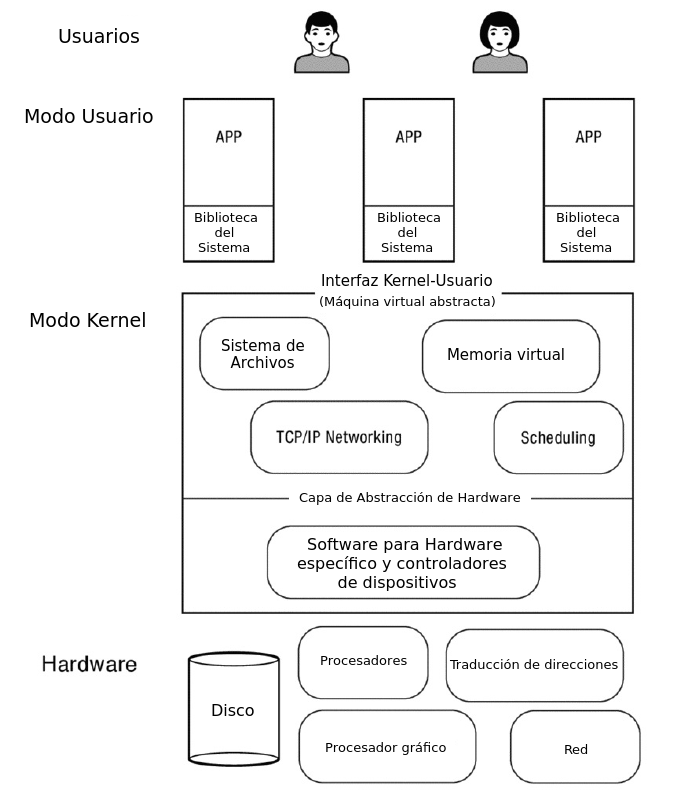
\includegraphics[scale=0.70]{img/fig0101}}
\caption{Sistema operativo de propósito general.}
\label{fig0101}
\end{figure}

Para sistemas de propósito general, los usuarios interactúan con aplicaciones, las aplicaciones se ejecutan en un entorno provisto por el sistema operativo y el sistema operativo media el acceso al hardware subyacente, como puede verse en la Figura \ref{fig0101}.

Para poder correr múltiples aplicaciones, el sistema operativo necesita desempeñar tres papeles:
\begin{enumerate}
\item \textbf{Arbitro} (\textit{Referee}). Los sistemas operativos administran los recursos compartidos entre diferentes aplicaciones ejecutándose en la misma máquina física. Por ejemplo, un sistema operativo
	\begin{itemize}
	\item Puede detener un programa e iniciar uno nuevo.
	\item Puede aislar aplicaciones entre sí, de forma que un error en una aplicación no corrompa otras aplicaciones ejecutándose en la misma máquina.
	\item Debe protegerse a sí mismo y a otras aplicaciones de virus de computadora maliciosos.
	\item Necesita decidir qué aplicaciones obtienen cuáles recursos y cuándo, dado que todas ellas comparten los recursos físicos de la computadora. 
	\end{itemize}
	
\item \textbf{Ilusionista}. Los sistemas operativos proveen una abstracción del hardware para facilitar el diseño de aplicaciones. Para escribir un programa en principio no se requeriría inferir sobre cuánta memoria física tiene el sistema o cuántos programas podrían estar compartiendo los recursos de la computadora. En cambio, los sistemas operativos proporcionan la ilusión de tener memoria casi ilimitada, a pesar de tener sólo una cantidad limitada de la misma. De la misma manera proporcionan la ilusión de que cada programa tiene todos los procesadores de la computadora para sí. Estas ilusiones permiten escribir programas independientemente de la cantidad de memoria física del sistema o de la cantidad física de procesadores. Dado que las aplicaciones son escritas a un nivel mayor de abstracción, el sistema operativo puede, casi de forma invisible, cambiar la cantidad de recursos asignados a cada aplicación.

\item \textbf{Pegamento}. Los sistemas operativos proporcionan un conjunto de servicios comunes que facilitan el intercambio de información entre aplicaciones. Como resultado de ello, \textit{cortar y pegar} funciona de manera uniforme en todo el sistema; un archivo escrito por una aplicación puede ser leído por otra. Muchos sistemas operativos proporcionan rutinas de interfaz de usuario comunes de modo que las aplicaciones pueden tener el mismo ``\textit{look and feel}''. Tal vez lo más importante, los sistemas operativos proporcionan una capa de separación de hardware de Entrada/Salida (I/O) de aplicaciones, de forma que estas últimas puedan escribirse de forma independiente del teclado, el ratón y la unidad de disco específicos en uso en un equipo determinado.
\end{enumerate}

\subsection{Recursos compartidos: el Sistema Operativo como Árbitro}
La administración de recursos compartidos es un tema central del uso de la mayoría de los sistemas operativos. Un usuario podría estar corriendo al mismo tiempo un navegador web, un reproductor multimedia y un procesador de texto, entre otros. El sistema operativo debe de alguna forma mantener estas actividades separadas y a su vez permitirle a cada una el uso de toda la capacidad de la máquina si las demás no se están ejecutando. Como mínimo, cuando un programa deja de ejecutarse el sistema operativo debiese permitir ejecutar otro programa. Mejor aún, el sistema operativo debiese poder permitir la ejecución al mismo tiempo de múltiples aplicaciones. El sistema operativo es un ejemplo de software desarrollado para realizar múltiples tareas a la vez.

Compartir recursos representa las siguientes ocupaciones al sistema operativo:
\begin{itemize}
\item \textbf{Asignación de recursos}. El sistema operativo debe mantener separadas todas las actividades simultáneas, asignándole a cada una de ellas recursos de manera apropiada. Una computadora usualmente dispone de unos pocos procesadores y una cantidad limitada de memoria, ancho de banda de red y espacio en disco. Al haber varias aplicaciones ejecutándose al mismo tiempo el sistema operativo debe decidir cuántos recursos entrega a cada una. No es una tarea trivial ya que, por ejemplo, si asigna muy poca memoria a una aplicación no sólo disminuirá el rendimiento de ésta, sino también el rendimiento general de otras aplicaciones.

\item \textbf{Aislamiento}. Un error en una aplicación no debiese interrumpir la ejecución de otras aplicaciones o del sistema operativo mismo. Esto se llama \textbf{aislamiento de fallas}, el cual requiere restringir el comportamiento de las aplicaciones. De otra forma cualquier aplicación descargada de la web, o cualquier scrpit embebido en una página web podría controlar completamente la máquina. Cualquier aplicación podría instalar \textit{spyware} en el sistema operativo para registrar cualquier pulsación de teclas hecha por el usuario o guardar la contraseña de cada sitio web visitado. Sin el aislamiento de fallas provisto por el sistema operativo, cualquier error en un programa podría corromper irremediablemente el disco.

\item \textbf{Comunicación}. La otra cara de aislamiento es la necesidad de comunicación entre las diferentes aplicaciones y diferentes usuarios. Por ejemplo, un sitio web puede ser implementado por un conjunto de aplicaciones que cooperan entre sí: una para seleccionar los anuncios publicitarios, otra para almacenar en caché los resultados recientes, otra para traer y combinar datos desde el disco, etc. Para que esto funcione, los diversos programas deben comunicarse entre sí. Si el sistema operativo impide que los errores y aplicaciones y usuarios maliciosos afecten a otros usuarios y sus aplicaciones, entonces ¿cómo hace también para soportar la comunicación y compartir los resultados? Al crear límites, un sistema operativo también debe permitir que esos límites puedan cruzarse con cuidado en maneras controladas cuando surja la necesidad.
\end{itemize}


\subsection{Limitaciones del enmascaramiento: el Sistema Operativo como Ilusionista}
Una segunda función importante de un sistema operativo es enmascarar las restricciones inherentes al hardware del ordenador. Las restricciones físicas limitan los recursos de hardware -- un ordenador tiene sólo un número limitado de procesadores y una cantidad limitada de memoria física, el ancho de banda de red y disco --. Además, como el sistema operativo debe decidir cómo dividir sus recursos fijos entre las diferentes aplicaciones
funcionando a cada momento, una aplicación particular puede tener diferentes cantidades de recursos cada cierto tiempo, incluso cuando se ejecutan en el mismo hardware.

La \textbf{virtualización} ofrece a una aplicación la ilusión de recursos que no están físicamente presentes. Por ejemplo, el sistema operativo puede proporcionar la abstracción que cada aplicación tiene un procesador dedicado, a pesar de que a nivel físico puede haber sólo un único procesador compartido entre todas las aplicaciones que se ejecutan en el equipo.

La mayoría de los recursos físicos pueden ser virtualizados. Por ejemplo, el hardware proporciona sólo una pequeña cantidad, finita, de memoria, mientras que el sistema operativo ofrece a las aplicaciones la ilusión de una cantidad casi infinita de memoria virtual. Las redes inalámbricas eliminan paquetes corruptos; el sistema operativo enmascara estas fallas para proporcionar la ilusión de un servicio confiable.

Algunos sistemas operativos virtualizan todo el equipo, ejecutando el sistema operativo como una aplicación encima de otro sistema operativo. Esto se conoce como crear una \textbf{máquina virtual}. El sistema operativo que se ejecuta en la máquina virtual, llamado el sistema operativo huésped, piensa que se está ejecutando en una máquina real, física, pero esto es una ilusión presentada por el verdadero sistema operativo que se ejecuta por debajo. Uno de los beneficios de una máquina virtual es la portabilidad de aplicaciones. Si un programa se ejecuta sólo en una versión antigua de un sistema operativo, aún puede trabajar en un nuevo sistema que ejecuta una máquina virtual.


\subsection{Proporcionando servicios en común: el Sistema Operativo como Pegamento}
Los sistemas operativos desempeñan un tercer papel fundamental: proporcionar un conjunto de servicios comunes, estándar a las aplicaciones para simplificar y estandarizar su diseño. Un ejemplo es el servidor web descrito anteriormente. El sistema operativo oculta los detalles de cómo funcionan los dispositivos de red y de disco, proporcionando una abstracción más simple basado en la recepción/envío de flujos fiables de bytes y la lectura/escritura de archivos con nombre. Esto le permite al servidor web enfocarse en su tarea principal --decodificar las peticiones entrantes y completarlas-- en lugar de formatear paquetes individuales la red y bloques de disco.

Una razón importante para que el sistema operativo proporcione servicios comunes, en lugar de dejar que cada aplicación proporcione los suyos, es facilitar el intercambio entre a las aplicaciones. La mayoría de los sistemas operativos también ofrecen una forma estándar a las aplicaciones para pasar mensajes y compartir la memoria.


\section{Evaluación del Sistema Operativo}
Después de haber definido lo que hace un sistema operativo, ¿cómo debemos elegir entre diseños alternativos? Se discuten varios criterios deseables para los sistemas operativos:
\begin{itemize}
\item \textbf{Fiabilidad y Disponibilidad}. ¿El sistema operativo hace lo que se requiere?
\item \textbf{Seguridad}. ¿Puede el sistema operativo ser dañado por un atacante?
\item \textbf{Portabilidad}. ¿El sistema operativo es fácil de instalar en nuevas plataformas de hardware?
\item \textbf{Actuación}. ¿Es la interfaz de usuario sensible, o el sistema operativo impone demasiadas sobrecargas?
\item \textbf{Adopción}. ¿Cuántos otros usuarios hay para este sistema operativo?
\end{itemize}

En muchos casos, las compensaciones entre estos criterios son inevitables: mejorar un sistema a lo largo de una dimensión puede perjudicarlo a lo largo de otro.

\subsection{Confiabilidad y Disponibilidad}
Tal vez la característica más importante de un sistema operativo es su confiabilidad. \textbf{Confiabilidad} significa que un sistema hace exactamente lo que está diseñado para hacer. En el nivel más bajo de software ejecutándose en el sistema, los errores del sistema operativo pueden tener efectos devastadores y ocultos. Si se rompe el sistema operativo, es posible que no pueda realizar su trabajo y, en algunos casos, puede incluso perderse el trabajo previo, por ejemplo, si el fallo daña los archivos en el disco. Por el contrario, los errores de aplicación pueden ser mucho más benignos, precisamente porque los sistemas operativos proporcionan el aislamiento de fallas y un reinicio rápido y limpio después de un error.

Hacer que un sistema operativo sea confiable es un reto. Los sistemas operativos a menudo operan en un entorno hostil, donde virus y otros códigos maliciosos tratan de tomar el control del sistema explotando errores de diseño o implementación de las defensas del sistema operativo.

La \textbf{disponibilidad} es el porcentaje de tiempo que el sistema es utilizable. Un sistema operativo con errores que frecuentemente se daña, perdiendo el trabajo del usuario, es a la vez no confiable y no disponible. Un sistema operativo con errores que frecuentemente se daña, pero nunca pierde el trabajo del usuario y no puede ser alterado por un ataque malicioso es confiable pero no disponible. Un sistema operativo que ha sido alterado pero aparenta seguir funcionando con normalidad no es confiable, pero está disponible.

De este modo, tanto la confiabilidad como la disponibilidad son deseables. La disponibilidad es afectada por dos factores: la frecuencia de fallos, medido como el tiempo medio hasta el fallo (MTTF: \textit{Mean Time To Failure}), y el tiempo que se necesita para restaurar un sistema a un estado de funcionamiento después de un fallo (por ejemplo, para reiniciar), llamado tiempo medio de reparación (MTTR: \textit{Mean Time To Repair}). La disponibilidad se puede mejorar mediante el aumento de la MTTF o reducir el MTTR.

\subsection{Seguridad}
Dos conceptos estrechamente relacionados con la confiabilidad son la seguridad y la privacidad. \textbf{Seguridad} significa que la operatoria del ordenador no puede ser comprometida por un atacante malintencionado. La \textbf{Privacidad} es un aspecto de la seguridad: los datos almacenados en el ordenador son sólo accesibles por usuarios autorizados.

Por desgracia, ningún ordenador útil es perfectamente seguro. Cualquier pieza compleja de software tiene errores, y los errores, en apariencia inocuos, pueden ser explotados por un atacante para obtener el control del sistema. O el hardware del ordenador puede ser manipulado, para proporcionar acceso al atacante. O el administrador del equipo podría ser poco fiable, utilizando sus credenciales para robar datos del usuario, etc.

Sin embargo, un sistema operativo puede ser, y debe ser, diseñado para minimizar su vulnerabilidad a los ataques. Por ejemplo, un fuerte aislamiento de fallos puede impedir que las aplicaciones de terceros tomen el control del sistema. Un \textbf{virus de computadora} es un programa de ordenador que modifica un sistema operativo o aplicación para copiarse a sí mismo desde un ordenador a otro sin el permiso o el conocimiento del propietario del ordenador. Una vez instalado en un ordenador, un virus a menudo proporciona el atacante el control de los recursos o los datos del sistema. Un ejemplo de virus informático es un \textit{keylogger}: un programa que modifica el sistema operativo para registrar cada pulsación de tecla introducida por el usuario y enviarlos de vuelta a la máquina del atacante. De esta manera, el atacante podría obtener acceso a las contraseñas del usuario, números de cuentas bancarias, y otra información privada.

Incluso con un fuerte aislamiento de fallos, un sistema puede ser inseguro si sus aplicaciones no están diseñadas para la seguridad. Por ejemplo un mensaje de correo electrónico puede parecer de alguien (tal vez alguien de confianza), cuando en realidad se trata del atacante y contiene, como un archivo adjunto, un virus malicioso.

Para complicar aún más las cosas, el sistema operativo no sólo debe impedir el acceso no autorizado a los datos compartidos, sino que también debe permitir el acceso en muchos casos. Los usuarios y los programas deben ser capaces de interactuar entre sí, de modo que es posible cortar y pegar texto entre diferentes aplicaciones, y para compartir los datos escritos en el disco o en la red.

Por lo tanto, un sistema operativo necesita tanto un mecanismo de aplicación y de una política de seguridad. Un \textbf{mecanismo de aplicación} es la forma en que el sistema operativo se asegura de que sólo se realicen acciones permitidas. La \textbf{política de seguridad} define lo que está permitido: quién está autorizado a acceder a qué datos, y quién puede realizar qué tipo de operaciones.

\subsection{Portabilidad}
Todos los sistemas operativos proporcionan aplicaciones con una abstracción del hardware subyacente; una abstracción portable es una que no cambia con cambios en el hardware. Un programa escrito para Microsoft Windows debería funcionar correctamente, independientemente de si se está utilizando una tarjeta gráfica específica, si el almacenamiento persistente se proporciona a través de la memoria flash o disco magnético rotatorio, o si la red es Bluetooth, Wi-Fi o Ethernet Gigabit.

La portabilidad también se aplica al propio sistema operativo. Es poco práctico reescribir sistemas operativos desde cero cada vez que se desarrolla un nuevo hardware o una nueva aplicación. En cambio, los nuevos sistemas operativos a menudo se derivan, al menos en parte, a partir de los antiguos. Como resultado, la mayoría de los sistemas operativos de éxito tienen un tiempo de vida medido en décadas. Esto significa que los sistemas operativos deben ser diseñados para soportar aplicaciones que aún no se han escrito y para ejecutarse en hardware que aún no ha sido desarrollado. Del mismo modo, los desarrolladores no quieren volver a escribir las aplicaciones cuando el sistema operativo es portado de una máquina a otra.

En el diseño de un sistema operativo para lograr la portabilidad, es de ayuda tener una forma simple y estándar para que  las aplicaciones interactúen con el sistema operativo. Una \textbf{máquina virtual abstracta} (AVM: \textit{Abstract Virtual Machine}) es la interfaz proporcionada por los sistemas a aplicaciones, incluyendo la operación de:
\begin{enumerate}
\item La interfaz de programación de aplicaciones (API: \textit{Application Programming Interface}) que es la lista de llamadas a funciones del sistema operativo proporcionada a las aplicaciones.
\item El modelo de acceso a la memoria.
\item El tipo y cantidad de instrucciones que pueden ser ejecutadas legalmente.
\end{enumerate}

Una AVM de un sistema operativo bien diseñada ofrece un punto fijo a través del cual tanto el código de aplicación y hardware pueden evolucionar de forma independiente. Esto es similar a la función del protocolo de Internet (IP) estándar en redes. Las aplicaciones distribuidas como el correo electrónico y la Web, escrita usando IP, están aislados de los cambios en la tecnología de red subyacente (Ethernet, Wi-Fi, etc.). Es igualmente importante que los cambios en las aplicaciones, desde el correo electrónico, la mensajería instantánea o el intercambio de ficheros, no requieran cambios simultáneos en el hardware subyacente.

El sistema operativo en sí mismo en gran medida se puede implementar de forma independiente de los detalles específicos del hardware. La interfaz que hace que esto sea posible se llama la capa de abstracción de hardware (HAL: \textit{Hardware Abstraction Layer}). Podría parecer que la AVM y la  HAL del sistema operativo son idénticas dado que ambas son capas portables diseñadas para ocultar los detalles de hardware. Sin embargo la AVM debe hacer más. Las aplicaciones se ejecutan en un contexto restringido, virtualizado y con acceso a servicios comunes de alto nivel, mientras que el propio sistema operativo utiliza una abstracción de procedimientos mucho más cercana al hardware real.

\subsection{Rendimiento}
Mientras que la portabilidad de un sistema operativo se hace evidente con el tiempo, el rendimiento de un sistema operativo es a menudo inmediatamente visible a sus usuarios. A pesar de que el rendimiento con frecuencia se asocia a cada aplicación individual, el diseño del sistema operativo puede afectar en gran medida el rendimiento percibido de la aplicación. El sistema operativo decide cuándo una aplicación se puede ejecutar, la cantidad de memoria que puede utilizar, y si sus archivos se almacenan en la memoria caché o agrupados de manera eficiente en el disco. Los sistemas operativos también median el acceso de las aplicaciones a la memoria, la red, y el disco. Debe evitar la ralentización de la ruta crítica, mientras que todavía proporciona el aislamiento de fallos necesario y el intercambio de recursos entre aplicaciones.

El rendimiento no es una sola cantidad. Más bien, se puede medir de varias maneras diferentes. 
\begin{itemize}
\item \textbf{Sobrecarga} (\textit{overhead}): es el costo de los recursos añadido a la implementación de una abstracción presentada a las aplicaciones. 
\item \textbf{Eficiencia}: es la falta de sobrecarga en una abstracción. Una manera de medir la sobrecarga (o inversamente, la eficiencia) es el grado en que la abstracción impide rendimiento de la aplicación. Supongamos que se podría ejecutar la aplicación directamente en el hardware subyacente, sin la sobrecarga de la abstracción del sistema operativo: ¿cuánto mejoraría el rendimiento de la aplicación?

\item \textbf{Equidad}: es la manera de dividir los recursos de forma equitativa entre los diferentes usuarios o aplicaciones que se ejecutan en la misma máquina. Esto plantea interrogantes a cómo debe decidir el sistema operativo si los recursos tienen que ser divididos en partes iguales entre los diferentes usuarios o aplicaciones, o si alguno de ellos debe percibir un trato preferencial.

\item \textbf{Tiempo de respuesta}: a veces llamado retardo, es el tiempo que tarda una sola tarea en ejecutarse, desde el momento en que comienza hasta que se completa. Por ejemplo, un tiempo de respuesta muy visible para ordenadores de escritorio es el tiempo desde que el usuario mueve el ratón hasta que el puntero en la pantalla refleja la acción del usuario. Un sistema operativo que proporciona tiempo de respuesta pobre puede ser inutilizable.

\item \textbf{Volumen de trabajo (throughput)}: es la velocidad a la que el sistema completa tareas. El throughput es una medida de la eficiencia para un grupo de tareas en lugar de una sola. Aunque podría parecer que los diseños que mejoran el tiempo de respuesta también lo hacen con el throughput, este no es el caso.

\item \textbf{Previsibilidad de rendimiento}: indica si el tiempo de respuesta del sistema u otra métrica es constante en el tiempo. La previsibilidad a menudo puede ser más importante que el rendimiento promedio. Si una operación de usuario a veces toma un instante, pero a veces mucho más tiempo, el usuario puede tener dificultades para adaptarse.
\end{itemize}


\subsection{Adopción}
Además de la fiabilidad, portabilidad y rendimiento, el éxito de un sistema operativo depende de dos factores fuera de su control inmediato: la amplia disponibilidad de las aplicaciones portadas a ese sistema operativo, y la amplia disponibilidad de hardware que el sistema operativo puede soportar.

El \textbf{efecto de red} se produce cuando el valor de una tecnología no sólo depende de sus capacidades intrínsecas, sino también del número de otras personas que lo han adoptado. Los diseñadores de aplicaciones y hardware invierten sus esfuerzos en las plataformas de sistemas operativos con la mayor cantidad de usuarios, mientras que los usuarios prefieren los sistemas operativos con las mejores aplicaciones o el hardware más barato. Más usuarios implican más aplicaciones y el hardware más barato; más aplicaciones y el hardware más barato implican a más usuarios, en un círculo virtuoso.

Un \textbf{sistema propietario} es uno bajo el control de una única empresa; puede ser cambiado en cualquier momento por su proveedor para satisfacer las necesidades de sus clientes. Un \textbf{sistema abierto} es aquel donde el código fuente del sistema es público, dando a cualquier persona la posibilidad de inspeccionar y cambiar el código. A menudo, un sistema abierto tiene una API que se puede cambiar con el acuerdo de un organismo público de normalización. La adhesión a las normas garantiza a los desarrolladores de aplicaciones que la API no será cambiada, excepto por acuerdo general. Por otra parte, los organismos de normalización pueden hacer que sea difícil para agregar rápidamente nuevas características solicitadas o requeridas. 

Ninguno de los dos sistemas, abiertos ni propietarias, son intrínsecamente mejor para su adopción. Windows y MacOS son sistemas operativos propietarios; Linux es un sistema operativo abierto. Los tres son ampliamente utilizados. Los sistemas abiertos son más fáciles de adaptar a una amplia variedad de plataformas de hardware, pero corren el riesgo de recaer en múltiples versiones, deteriorando el efecto de red. Los proveedores de sistemas operativos propietarios argumentan que sus sistemas son más fiables y mejor adaptados a las necesidades de sus clientes. Los problemas de interoperabilidad pueden ser reducidos si la misma empresa controla tanto el hardware como el software, pero la limitación de un sistema operativo a una plataforma de hardware perjudica el efecto de red y podría alejar a los consumidores.

\subsection{Compromisos de Diseño}
La mayoría de los diseños prácticos de sistemas operativos establecen un equilibrio entre los objetivos de confiabilidad, seguridad, portabilidad, rendimiento y adopción. Las opciones de diseño que mejoran la portabilidad -- por ejemplo, la preservación de las interfaces heredadas -- a menudo hacen que el sistema sea en su conjunto menos confiable y menos seguro. Del mismo modo, a menudo es posible aumentar el rendimiento del sistema mediante la ruptura de una abstracción. Sin embargo, este tipo de optimizaciones de rendimiento pueden añadir complejidad y, por lo tanto, potencialmente dañar la confiabilidad. El diseñador del sistema operativo debe sopesar cuidadosamente estos objetivos en conflicto.


\section{Sistemas Operativos: Pasado, Presente y Futuro}

\subsection{Impacto de las tendencias tecnológicas}
El aspecto más sorprendente de los últimos cincuenta años en la tecnología informática ha sido el efecto acumulativo de la Ley de Moore y los avances comparables en las tecnologías relacionadas, como la memoria y almacenamiento en disco. La \textbf{Ley de Moore} establece que la densidad de transistores aumenta exponencialmente con el tiempo; mejoras exponenciales similares han ocurrido en muchas otras tecnologías de componentes.

Desde 1981 a la actualidad el costo de procesamiento y la memoria se ha reducido en casi seis órdenes de magnitud; el costo de la capacidad del disco se ha reducido en siete órdenes de magnitud. No todas las tecnologías han mejorado en la misma proporción; la latencia de disco ha mejorado, pero a un ritmo mucho más lento que la capacidad del disco. Estos cambios relativos han alterado radicalmente tanto el uso de las computadoras y las ventajas y desventajas que enfrentan los diseñadores de sistemas operativos.

En los primeros años de la informática, los ordenadores eran más caros que los salarios de las personas que los utilizan. Los usuarios hacían cola esperando su turno para ejecutar un programa. Con el tiempo, las computadoras se han vuelto lo suficientemente baratas como para permanecer inactivas hasta que las necesitemos.

A pesar de estos cambios, los sistemas operativos todavía se enfrentan a los mismos retos conceptuales como lo hicieron hace cincuenta años. Para gestionar los recursos informáticos para aplicaciones y usuarios, se deben asignar los recursos entre aplicaciones, proporcionar aislamiento de fallos y servicios de comunicación, proveer limitaciones abstractas de hardware, etc. Aunque no se sabe con precisión cómo la tecnología informática o la demanda de aplicaciones van a evolucionar, es muy probable que persistan estos retos fundamentales de los sistemas operativos.

\subsection{Primeros Sistemas Operativos}
Los primeros sistemas operativos eran bibliotecas de ejecución destinadas a simplificar la programación de los primeros sistemas informáticos. Los primeros ordenadores a menudo ocupaban toda una planta de un depósito, costaban millones de dólares, y sin embargo, eran capaces de ser utilizados sólo por una persona a la vez. El usuario primero restablecía el sistema, cargaba el programa conmutando en el sistema de un solo bit a la vez, y pulsaba '\textit{go}', produciendo la salida para ser estudiada minuciosamente durante el turno del siguiente usuario. Si el programa tenía un error, el usuario tendría que esperar a probar la ejecución otra vez.

Los primeros sistemas operativos se desarrollaron como una forma de reducir los errores al proporcionar un conjunto estándar de servicios comunes. Por ejemplo, los primeros sistemas operativos proporcionaban rutinas estándar de entrada/salida (E/S) que cada usuario podía vincular a sus programas. Estos servicios hacían que fuera más probable que el programa de un usuario produjera una salida útil.

\subsection{Sistemas Operativos Multi-Usuario}
El siguiente paso fue compartir. Cuando el tiempo de procesamiento es valioso, restringir el uso del sistema a un usuario a la vez es un desperdicio. Por ejemplo, en los primeros sistemas el procesador quedaba inactivo mientras el usuario cargaba el programa. Un \textbf{sistema operativo por lotes (batch)} funciona con una cola de tareas. Se ejecuta un bucle simple: cargar, ejecutar, y descargar cada trabajo por vez. Mientras que un trabajo ya está en marcha, el sistema operativo configura los dispositivos de E/S para hacer transferencias de fondo para el trabajo siguiente/anterior mediante un proceso denominado acceso directo a memoria (DMA: \textit{Direct Memory Access}). Con DMA, el dispositivo de E/S transfiere sus datos directamente a la memoria en un lugar especificado por el sistema operativo. Cuando la transferencia de E/S se completa, el hardware interrumpe el procesador, transfiriendo el control al manejador de interrupciones del sistema operativo. El sistema operativo inicia la siguiente transferencia de DMA y luego continúa con la ejecución de la aplicación. La interrupción se muestra a la aplicación como si no hubiera pasado nada, salvo algún retraso entre una instrucción y la siguiente.

Los sistemas operativos por lotes pronto se extendieron para ejecutar varias aplicaciones a la vez. Esto se llamó \textbf{multitarea} o, a veces \textbf{multiprogramación}. Múltiples programas se cargan en la memoria al mismo tiempo, cada uno listo para usar el procesador si por cualquier razón la tarea anterior necesita hacer una pausa, por ejemplo, para leer la entrada adicional o producir de salida. La multitarea aumenta la eficiencia del procesador a casi el 100 \%. Sin embargo, el uso compartido de procesador plantea la necesidad de aislamiento de programas, para evitar que un error en un programa dañe o corrompa otro. Durante este período, los diseñadores de computadoras añaden protección de memoria de hardware, para reducir la sobrecarga (overhead) del aislamiento de fallos.

Un desafío práctico con la computación por lotes, sin embargo, es cómo depurar el sistema operativo en sí mismo. A diferencia de un programa de aplicación, un sistema operativo por lotes asume que está en control directo del hardware. Las nuevas versiones sólo pueden ser probadas al detener todas las aplicaciones y reiniciar el sistema, esencialmente equivale a volver al esquema de ordenador con un sistema operativo de un solo usuario.


\subsection{Sistemas Operativos de Tiempo Compartido}
Con el tiempo, el efecto acumulativo de la Ley de Moore significó que el coste de la computación se redujera al punto donde los sistemas podrían ser optimizados para los usuarios en lugar de para un uso eficiente del procesador. UNIX, por ejemplo, se convirtió en la base para sistemas operativos como Apple MacOS X, Linux y Android de Google, entre otros.

Los \textbf{sistemas operativos de tiempo compartido} -- como Windows, MacOS o Linux -- están diseñados para soportar el uso interactivo de la computadora en lugar del procesamiento por lotes de los sistemas anteriores. Con el tiempo compartido, la entrada es suministrada por un usuario mientras escribe en un teclado o utiliza otro dispositivo de entrada conectado directamente al ordenador. Cada pulsación de tecla o acción del ratón provoca una interrupción indicándole un evento al procesador; el controlador de interrupciones lee el evento desde el dispositivo y lo pone en cola dentro del sistema operativo. Cuando la aplicación reanuda, se obtiene el evento desde el sistema operativo, se procesa y se modifica el display (e.g. pantalla del monitor) debidamente antes de ir a buscar el próximo evento. Cientos o incluso miles de tales eventos pueden ser procesados por segundo, lo que requiere que tanto el sistema operativo como la aplicación se diseñen para ráfagas frecuentes de muy corta actividad en vez del modelo de ejecución sostenida del procesamiento por lotes.

Los primeros sistemas de tiempo compartido permitieron tener muchos usuarios en simultáneo, pero incluso esto fue sólo una fase. Con el tiempo, las computadoras se volvieron lo suficientemente baratas como para que las personas pudieran permitirse sus propios ordenadores ``personales'' dedicados. El acceso a los datos compartidos se convirtió en primordial, consolidando el cambio a la computación cliente-servidor.


\subsection{Sistemas Operativos Modernos}
Hoy en día, existe una gran diversidad de dispositivos de cómputo, con diferentes sistemas operativos que se ejecutan en ellos. Las ventajas y desventajas que enfrenta un diseñador de sistemas operativos dependen de las capacidades físicas del hardware, así como las necesidades de aplicación y de usuario. Los siguientes son algunos ejemplos de sistemas operativos modernos.

\begin{itemize}
\item \textbf{Sistemas Operativos de Escritorio, Laptop y Netbook}

Ejemplos incluyen Windows, MacOS y Linux. Estos sistemas son de un solo usuario, ejecutan muchas aplicaciones y tienen varios dispositivos de E/S. Los sistemas operativos iniciales para PCs tenían una capacidad muy limitada para aislar diferentes partes del sistema de las demás. Con el tiempo, sin embargo, se hizo evidente que se necesitaba un aislamiento de fallos más estricto para mejorar la confiabilidad del sistema y la resistencia contra los virus informáticos. Otros objetivos clave de diseño para estos sistemas incluyen la adopción (para apoyar un amplio conjunto de aplicaciones) y el rendimiento interactivo.

\item \textbf{Sistemas Operativos para \textit{Smartphones}}

Un \textit{smartphone} es un teléfono móvil con un ordenador incorporado capaz de ejecutar aplicaciones de terceros. Ejemplos de sistemas operativos de \textit{smartphones} incluyen iOS, Android y Windows Phone. Los teléfonos inteligentes tienen sólo un usuario, pero deben ser compatibles con muchas aplicaciones. Objetivos clave de diseño incluyen la capacidad de respuesta, el soporte a una amplia variedad de aplicaciones, y el uso eficiente de la batería. Otro objetivo de diseño es la privacidad del usuario. Debido a que las aplicaciones de terceros pueden recopilar datos privados sigilosamente con fines de comercialización, como la lista de contactos del usuario, el sistema operativo debe estar diseñado para limitar el acceso a los datos protegidos del usuario.

\item \textbf{Sistemas Operativos para Servidores}

Los motores de búsqueda, medios de comunicación web, sitios de comercio electrónico, y sistemas de correo electrónico están alojados en los equipos de los centros de datos; cada uno de estos ordenadores ejecuta un sistema operativo, a menudo una versión de potencia industrial de uno de los sistemas de escritorio descritos anteriormente. Por lo general, sólo una única aplicación, como un servidor web, se ejecuta por máquina, pero el sistema operativo debe coordinar miles de conexiones de red entrantes simultáneas. El rendimiento en el manejo de un gran número de solicitudes por segundo es un objetivo clave de diseño. Al mismo tiempo, hay una bonus en la capacidad de respuesta. Los servidores también operan en un ambiente hostil, donde los atacantes maliciosos pueden intentar alterar o bloquear el servicio; la resistencia al ataque es un requisito esencial.

\item \textbf{Máquinas Virtuales}

Un monitor de máquina virtual es un sistema operativo que puede ejecutar otro sistema operativo como si se tratara de una aplicación. Los ejemplos incluyen VMware, Xen y Windows Virtual PC. Los monitores de máquinas virtuales enfrentan muchos de los mismos problemas que otros sistemas operativos, con el reto añadido que supone la coordinación de un conjunto de coordinadores. Un sistema operativo huésped en ejecución en una máquina virtual toma decisiones de asignación de recursos y de aislamiento de fallas como si estuviera en completo control de sus recursos, a pesar de que está compartiendo el sistema con otros sistemas operativos y aplicaciones.

\item \textbf{Sistemas Embebidos}

Con el tiempo, las computadoras se han vuelto lo suficientemente baratas para integrarse a cualquier número de dispositivos de consumo, desde decodificadores de televisión por cable a sistemas de control para automóviles y aviones. Los dispositivos embebidos suelen ejecutar un sistema operativo personalizado incluido con software específico para las tareas que controla el dispositivo. Merecen mucha atención, ya que los errores de software en ellos pueden tener efectos devastadores.

\item \textbf{Clústeres de Servidores}

Para tolerancia a fallos, escala y capacidad de respuesta, los sitios web se implementan cada vez más en clústeres de ordenadores alojados en uno o más centros de datos distribuidos geográficamente en ubicaciones cercanas a los usuarios. Si un equipo falla debido a un desperfecto de hardware, error de software o interrupción en la alimentación, otro equipo puede hacerse cargo de su función. Si la demanda para el sitio Web supera lo que un solo equipo puede manejar, las peticiones web se pueden dividir entre varias máquinas. Al igual que con los sistemas operativos normales, las aplicaciones de clústeres de servidores se ejecutan en la parte superior de una interfaz de clúster abstracto para aislar la aplicación de cambios de hardware y para evitar que fallos en una aplicación afecten a otras aplicaciones en el mismo centro de datos. Del mismo modo, los recursos pueden ser compartidos entre: (1) varias aplicaciones en el mismo sitio web (como Google Search, Google Earth, y Gmail), y (2) varios sitios web alojados en el mismo hardware del clúster (por ejemplo, Compute Engine de Google).
\end{itemize}


\subsection{Sistemas Operativos Futuros}
En primer lugar, dado que pueden presentarse desafíos de seguridad y confiabilidad, potenciales enormes beneficios podrían ser el resultado de tener computadoras controladas firmemente y poder coordinar la infraestructura física, como la red eléctrica, la red telefónica, y los dispositivos médicos y sistemas de registros médicos de un hospital. En segundo lugar, los cambios en el hardware subyacente a menudo desencadenan un nuevo trabajo en el diseño de sistemas operativos. El futuro de los sistemas operativos es también el futuro de hardware:

\begin{itemize}
\item Centros de cómputos a muy gran escala.
\item Sistema multi-núcleo a muy gran escala.
\item Dispositivos informáticos portátiles multi-funcionales ubicuos (portables a todas partes).
\item Sistemas muy heterogéneos (como todos los dispositivos se vuelven programables, se necesitarán sistemas operativos para una gran variedad de dispositivos, desde los superordenadores a los refrigeradores).
\item Almacenamiento a muy gran escala.
\end{itemize}

\clearpage

\chapter{La Abstracción del Kernel}
Un rol central de los sistemas operativos es la \textbf{protección} -- el aislamiento de aplicaciones y usuarios potencialmente dañinos para evitar que corrompan otras aplicaciones o el propio sistema operativo. La protección es esencial para lograr algunos de los objetivos mencionados antes:
\begin{itemize}
\item Confiabilidad
\item Seguridad
\item Privacidad
\item Asignación de recursos equitativa
\end{itemize}

La implementación de la protección es el trabajo del kernel o núcleo del sistema operativo. El \textbf{kernel}, el nivel más bajo de software que se ejecuta en el sistema, tiene acceso completo a todo el hardware de la máquina. El núcleo es de confianza, necesariamente para poder hacer cualquier cosa con el hardware. El resto -- es decir, el software que se ejecuta en el sistema que no es de confianza -- se ejecuta en un entorno restringido con menos que el completo acceso a toda la potencia del hardware.

Por su parte, las aplicaciones en sí a menudo necesitan ejecutar código no confiable de terceros de manera segura. Un ejemplo es un navegador web que ejecuta código \textit{JavaScript} integrado para elaborar una página web. Sin protección, un \textit{script} con un virus incrustado puede tomar el control del navegador, por lo que los usuarios piensan que están interactuando directamente con la web, cuando en realidad sus contraseñas web podrían estar siendo desviadas a un atacante.

Un \textbf{proceso} es la ejecución de un programa de aplicación con derechos restringidos; el proceso es la abstracción de ejecución protegida proporcionada por el kernel del sistema operativo. Un proceso necesita el permiso del kernel del sistema operativo antes de acceder a la memoria de cualquier otro proceso, antes de leer o escribir en el disco, antes de cambiar la configuración de hardware, y así sucesivamente. En otras palabras, el kernel del sistema operativo arbitra y controla el acceso de cada proceso al hardware.

El kernel del sistema operativo se ejecuta directamente en el procesador con derechos ilimitados. El kernel puede realizar cualquier operación disponible en el hardware. Las aplicaciones necesitan ejecutarse en el procesador con todas las operaciones potencialmente peligrosas deshabilitadas. Para que esto funcione, el hardware necesita proporcionar un poco de ayuda. Tanto el kernel del sistema operativo como los procesos de las aplicaciones --que se ejecutan con derechos restringidos-- comparten la misma máquina: el mismo procesador, la misma memoria y el mismo disco.


\section{La Abstracción del Proceso}
Un programador escribe código en un lenguaje de alto nivel. Un compilador convierte el código en una secuencia de instrucciones de máquina y almacena esas instrucciones en un archivo, llamado \textbf{imagen ejecutable} del programa. El compilador también define los datos estáticos que el programa necesita, junto con sus valores iniciales, y los incluye en la imagen ejecutable.

Para ejecutar el programa, el sistema operativo copia las instrucciones y los datos de la imagen ejecutable en la memoria física. El sistema operativo deja de lado una región de memoria, la \textbf{pila de ejecución}, para mantener el estado de las variables locales durante las llamadas de procedimiento. El sistema operativo también deja de lado una región de memoria, llamada \textbf{heap}, para cualquier estructura de datos asignada dinámicamente que podría necesitar el programa. Por supuesto, para copiar el programa en la memoria, el sistema operativo mismo debe estar ya cargado en la memoria, con su propia pila y \textit{heap}. Ignorando la protección, una vez que un programa se carga en memoria, el sistema operativo puede iniciarlo ajustando el puntero de pila y el salto a la primera instrucción de programa. El propio compilador es un programa más: el sistema operativo inicia el compilador insertando su imagen ejecutable en la memoria y saltando a su primera instrucción.


Para ejecutar varias copias del mismo programa, el sistema operativo puede hacer múltiples copias de las instrucciones del programa, datos estáticos, \textit{heap} y la pila en la memoria. La mayoría de los sistemas operativos reutilizan la memoria siempre que sea posible: almacenan sólo una única copia de las instrucciones de un programa cuando múltiples copias del programa se ejecutan al mismo tiempo. A pesar de ello, se necesita una copia separada de los datos del programa, \textit{heap} y pila.

Por lo tanto, un proceso es un ejemplo de un programa, de la misma manera que un objeto es una instancia de una clase en la programación orientada a objetos. Cada programa puede tener cero, uno o más procesos en ejecución Para cada instancia de un programa, hay un proceso con su propia copia del programa en la memoria.

El sistema operativo lleva un registro de los diversos procesos en el equipo utilizando una estructura de datos llamada bloque de control de proceso, o PCB (\textit{Process Control Block}). Los PCB almacenan toda la información que el sistema operativo necesita acerca de un proceso en particular: dónde se almacena en la memoria, en qué parte del disco reside su imagen ejecutable, qué usuario solicitó ejecutarlo, qué privilegios tiene el proceso, etc.

Algunos programas se componen de múltiples actividades simultáneas, o hilos. Un navegador web, por ejemplo, podría necesitar recibir la entrada del usuario, al mismo tiempo que se está dibujando la pantalla o recibiendo entrada de red. Cada una de estas actividades por separado tiene su propio contador de programa y pila, pero opera en el mismo código y datos como los demás hilos. El sistema operativo ejecuta múltiples hilos en un proceso, en la misma forma que ejecuta varios procesos en la memoria física.

\textbf{Procesos, procesos ligeros e hilos}

Un hilo (\textit{thread}) es una secuencia lógica de instrucciones que ejecutan tanto el sistema operativo como los códigos de aplicación. Un programa multiprocesador puede tener varias secuencias de instrucciones que se ejecutan en paralelo, cada uno con su propio contador de programa, pero todos cooperando dentro de un único límite de protección. Durante un tiempo, éstos fueron llamados ``procesos ligeros'' (cada uno es una secuencia de instrucciones que cooperan dentro de un límite de protección), pero con el tiempo la palabra ``hilo'' se volvió más ampliamente utilizada.

Esto conduce a la convención de nombres actualmente utilizada en casi todos los sistemas operativos modernos: \textbf{un \textit{proceso} ejecuta un \textit{programa}, que consta de uno o más \textit{hilos} que se ejecutan dentro de un \textit{límite de protección}}.


\section{El Modo Dual de Operación}
Una vez que un programa se carga en memoria y el sistema operativo inicia el proceso, el procesador trae una instrucción por vez; a continuación la decodifica y ejecuta. Algunas instrucciones calculan valores, por ejemplo, al multiplicar dos registros y poner el resultado en otro registro. Algunas instrucciones leen o escriben ubicaciones en la memoria. Y otras instrucciones, como las ramas (saltos/\textit{branches}) o las llamadas de procedimiento, cambian el contador de programa y de este modo determinan la siguiente instrucción a ejecutar.

\begin{figure}[tbhp]
\centerline{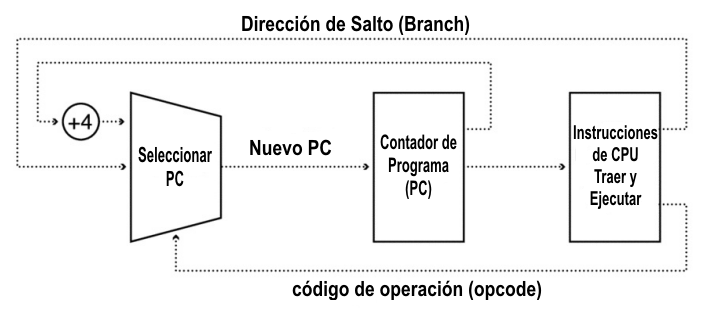
\includegraphics[scale=0.70]{img/fig0201}}
\caption{La operación básica de una CPU.}
\label{fig0201}
\end{figure}

Ahora, ¿cómo el kernel del sistema operativo evita que un proceso dañe otros procesos o el propio sistema operativo? Después de todo, cuando múltiples programas se cargan en la memoria al mismo tiempo, ¿qué impide que un proceso sobrescriba las estructuras de datos de otro proceso, o incluso sobrescriba la imagen del sistema operativo almacenado en el disco? La mayoría de las instrucciones son perfectamente seguras, tales como la adición de dos registros y almacenar el resultado en un tercer registro. ¿Se puede modificar el procesador de alguna manera para permitir que las instrucciones seguras se ejecuten directamente en el hardware? Para lograr esto, se implementa el denominado \textbf{modo dual de operación}, representado por un único bit en el registro de estado del procesador que indica el modo actual del procesador. En el \textbf{modo de usuario}, el procesador comprueba cada instrucción antes de ejecutarla para verificar que está permitida para ser realizada por ese proceso. En \textbf{modo de kernel}, el sistema operativo se ejecuta con los controles de protección apagados.

\textit{\textbf{El kernel vs. el resto del sistema operativo}}

El kernel es una pieza fundamental de un sistema operativo, pero es sólo una parte del sistema operativo en general. En la mayoría de los sistemas operativos modernos, una parte del mismo se ejecuta en modo de usuario como una biblioteca vinculada a cada aplicación. Un ejemplo es el código de la biblioteca que gestiona los botones de menú de una aplicación. El código de la biblioteca (pero no el kernel del sistema operativo) \textit{comparte el mismo destino} que el resto de la aplicación: un problema con uno tiene el mismo efecto que un problema con el otro.

Del mismo modo, partes del sistema operativo pueden ejecutarse en sus propios procesos a nivel de usuario. Un gestor de ventanas es un ejemplo. El gestor de ventanas dirige las acciones del ratón y la entrada de teclado que se producen dentro de una ventana a la aplicación correcta, y el administrador también se asegura de que cada aplicación modifique sólo la parte de la pantalla correspondiente a la aplicación, y no la barra de menús del sistema operativo o cualquier otra ventana de aplicación. Sin esta restricción, una aplicación maliciosa podría tomar el control de la máquina. Por ejemplo, un virus podría presentar una pantalla de login que luzca idéntica a la del sistema, lo que podría inducir a los usuarios a revelar sus contraseñas al atacante.

Otro motivo para tener separado del kernel al resto del sistema operativo (código de bibliotecas y cualquier aplicación de nivel usuario) es que a menudo es más fácil de depurar el código de nivel de usuario que el código del kernel. Más importante aún, el kernel debe ser de confianza, ya que tiene control total sobre el hardware. Cualquier error en el kernel puede corromper el disco, la memoria de otras aplicaciones, o simplemente bloquear el sistema. Al separar el código que no necesita estar en el kernel, el sistema operativo puede ser más confiable -- un error en el sistema de ventanas es bastante malo, pero sería aún peor si se podría corromper el disco. Esto ilustra el \textbf{principio de mínimo privilegio}: la seguridad y la confiabilidad aumentan si cada parte del sistema tiene exactamente los privilegios que necesita para hacer su trabajo, y nada más.

\begin{figure}[tbhp]
\centerline{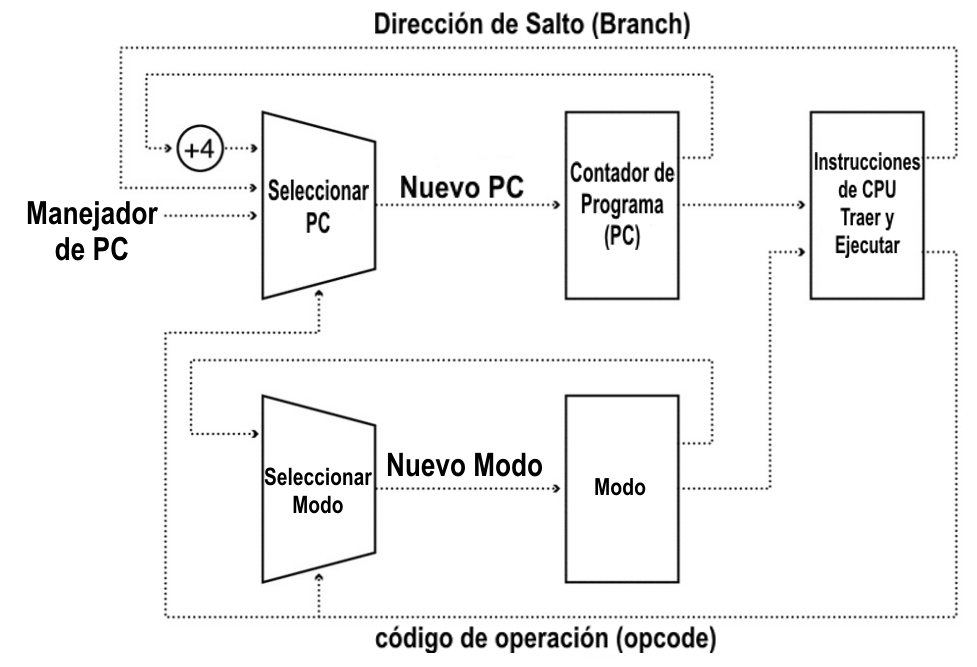
\includegraphics[scale=0.54]{img/fig0202}}
\caption{El funcionamiento de una CPU con los modos kernel y usuario.}
\label{fig0202}
\end{figure}

En la Figura \ref{fig0202} se muestra el funcionamiento de un procesador de modo dual; el contador de programa y el bit de modo juntos controlan el funcionamiento del procesador. A su vez, el bit de modo es modificado por algunas instrucciones, tal como el contador de programa es modificado por algunas instrucciones. Para permitir al kernel del sistema operativo proteger las aplicaciones y los usuarios unos de otros, pero también dejar que código de usuario se ejecute directamente en el procesador, como mínimo, el hardware debe ser compatible con tres cosas:

\begin{itemize}
\item \textbf{Instrucciones privilegiadas}: todas las instrucciones potencialmente inseguras están prohibidas cuando se ejecutan en modo usuario.
\item \textbf{Protección de memoria}: todos los accesos a memoria fuera de la región de memoria válida de un proceso están prohibidos cuando se ejecutan en modo usuario.
\item \textbf{Interrupciones del temporizador}: independientemente de lo que hace el proceso, el kernel debe tener una manera de recuperar periódicamente el control del proceso actual.
\end{itemize}

Además, el hardware también debe proporcionar una forma de transferir de forma segura de control de modo usuario a modo kernel y viceversa.


\subsection{Instrucciones Privilegiadas}
El aislamiento de procesos es posible sólo si hay una manera de limitar los programas que se ejecutan en modo usuario de cambiar directamente su nivel de privilegio. Los procesos pueden indirectamente cambiar su nivel de privilegio mediante la ejecución de una instrucción especial, denominada \textbf{llamada al sistema}, para transferir el control al kernel desde una ubicación fija definida por el sistema operativo. Aparte de la transferencia de control al kernel del sistema operativo (esto es, en efecto, convertirse en el kernel) en estas ubicaciones fijas, un proceso de aplicación no puede cambiar su nivel de privilegio.

Otras instrucciones también se limitan a ser utilizadas sólo por código del kernel. No se puede permitir que la aplicación cambie el conjunto de ubicaciones de memoria a las que puede acceder. Limitar a una aplicación a que acceda sólo a su propia memoria es esencial para evitar que, de forma deliberada o accidental, se dañe o se de un mal uso de los datos o código de otras aplicaciones o el sistema operativo en sí. Además, las aplicaciones no pueden deshabilitar las interrupciones del procesador.

Las instrucciones disponibles en el modo kernel, pero no en el modo usuario se llaman \textbf{instrucciones privilegiadas}. El kernel del sistema operativo debe ser capaz de ejecutar estas instrucciones para realizar su trabajo -- necesarias para cambiar los niveles de privilegios, ajustar el acceso a memoria y activar/desactivar las interrupciones. Si estas instrucciones estuvieran disponibles para las aplicaciones, luego una aplicación maliciosa podría tomar el control del kernel del sistema operativo.

Si una aplicación intenta acceder a memoria restringida o intenta cambiar su nivel de privilegio, esto causa una \textbf{excepción de procesador}. A diferencia de un lenguaje de programación que maneja una excepción en tiempo de ejecución y utilizando código de usuario, una excepción de procesador hace que el procesador transfiera el control a un manejador de excepciones en el kernel del sistema operativo. Por lo general el kernel simplemente detiene el proceso después de una violación de privilegios.


\subsection{Protección de Memoria}
Para ejecutar un proceso de aplicación, tanto en el sistema operativo como la aplicación deben residir en la memoria al mismo tiempo. La aplicación debe estar en la memoria con el fin de ejecutarse, mientras que el sistema operativo debe estar allí para iniciar el programa y para manejar las interrupciones, excepciones del procesador o llamadas al sistema que se producen mientras se ejecuta el programa. Además, se pueden almacenar también otros procesos de aplicación en la memoria.

Para compartir memoria de forma segura, el sistema operativo debe ser capaz de configurar el hardware para que cada proceso de aplicación pueda leer y escribir sólo su propia memoria, no la memoria del sistema operativo o cualquier otra aplicación. De lo contrario, una aplicación podría modificar el código o los datos del kernel del sistema operativo para obtener el control sobre el sistema.

En la Figura \ref{fig0203} se ilustra el principio general para impedir el acceso a un programa de usuario a partes de la memoria física. 
Con este enfoque, un procesador tiene dos registros adicionales, llamados \textbf{base y límite}. La base especifica el inicio de la región de memoria del proceso en la memoria física, mientras que el límite da su punto final. Estos registros pueden ser modificados por instrucciones privilegiadas, es decir, por el sistema operativo que se ejecuta en modo kernel. El código de nivel usuario no puede cambiar los valores de estos registros.

\begin{figure}[tbhp]
\centerline{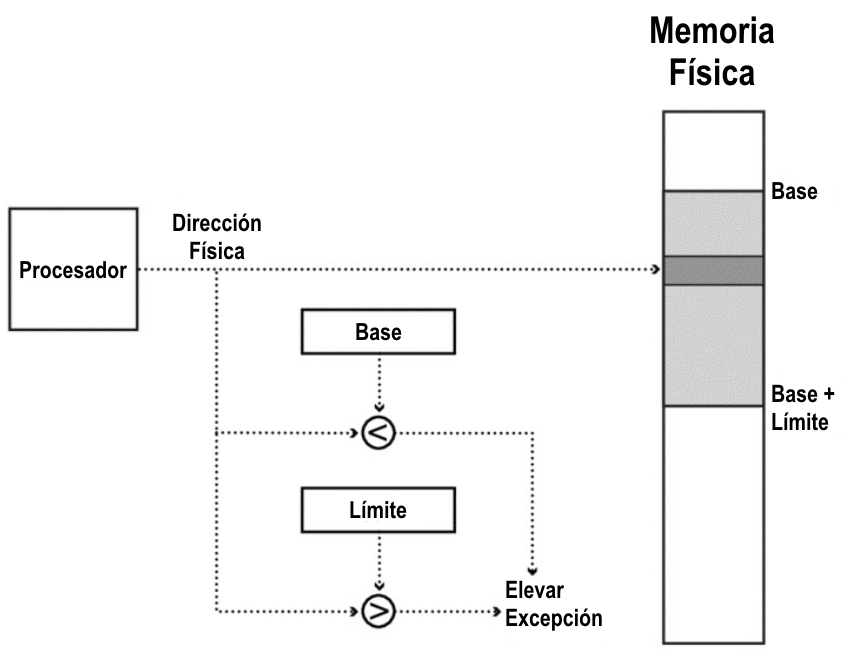
\includegraphics[scale=0.55]{img/fig0203}}
\caption{Método Base-Límite de protección de memoria usando direcciones físicas.}
\label{fig0203}
\end{figure}

Cada vez que el procesador obtiene una instrucción, se comprueba la dirección del contador de programa para ver si está entre los registros base y límite. Si es así, se permite proceder a la instrucción FETCH (obtener/traer); de otro modo, el hardware genera una excepción, se suspende el programa y se transfiere el control de vuelta al kernel del sistema operativo. Del mismo modo, para instrucciones que leen o escriben datos en la memoria, el procesador comprueba cada referencia a la memoria contra los registros base y límite, lo que genera una excepción de procesador si se violan los límites.

El kernel del sistema operativo se ejecuta sin los registros base y límite, lo que le permite acceder a cualquier memoria en el sistema - la memoria del kernel o la memoria de cualquier proceso de aplicación que se ejecuta en el sistema. Dado que las aplicaciones tocan sólo su propia memoria, el núcleo debe copiar explícitamente cualquier entrada o salida dentro o fuera de la región de memoria de la aplicación.

El uso de los registros base y límite, direccionados físicamente, puede proporcionar protección pero esto no proporciona algunas características importantes:

\begin{itemize}
\item \textbf{\textit{Heap} y pila expandibles}: con un sólo par de registros base y límite por cada proceso, la cantidad de memoria asignada a un programa se fija cuando se inicia el programa.
\item \textbf{Memoria compartida}: los registros base y límite no permiten que la memoria sea compartida entre los diferentes procesos, como sería útil, por ejemplo, para compartir código entre múltiples procesos que ejecutan el mismo programa o usan la misma biblioteca.
\item \textbf{Direcciones de memoria física}: cada programa se carga en la memoria física en tiempo de ejecución y debe utilizar esas direcciones de memoria física. Puesto que un programa puede ser cargado en diferentes lugares dependiendo de qué otros programas se estén ejecutando al mismo tiempo, el kernel debe cambiar la ubicación de cada instrucciones y dato que referencie a una dirección global, cada vez que el programa se carga en memoria.
\item \textbf{Fragmentación de memoria}: Una vez que se inicia un programa, es casi imposible reubicarlo. El programa podría almacenar punteros en los registros o en la pila de ejecución y estos punteros necesitan ser cambiados para mover el programa a una región diferente de la memoria física. Con el tiempo, a medida que las aplicaciones comienzan y terminan en tiempos irregulares, la memoria se fragmentará cada vez más. Potencialmente, la fragmentación de memoria puede llegar a un punto donde no hay suficiente espacio contiguo para iniciar un nuevo proceso, a pesar de suficiente memoria libre en su conjunto.
\end{itemize}

Por estas razones, la mayoría de los procesadores modernos introducen un nivel de indirección, denominado \textbf{direcciones virtuales}. Con direcciones virtuales, la memoria de cada proceso se inicia en el mismo lugar, por ejemplo, cero. Cada proceso cree que tiene toda la máquina para sí aunque, obviamente, esto no sea la realidad. El hardware traduce estas direcciones virtuales a posiciones de memoria física. Las direcciones virtuales también pueden dejar que la pila y \textit{heap} comiencen en extremos separados del espacio de direcciones virtuales para que puedan crecer según las necesidades del programa. La expansión es completamente transparente para el proceso de usuario
 
Con direcciones virtuales, si varias copias de un programa se ejecutan simultáneamente, cada copia del programa imprimirá exactamente el mismo resultado. Esto sería imposible si cada copia se dirigiera directamente las posiciones de memoria física. En otras palabras, cada instancia del programa parece encontrarse en su propia copia completa de la memoria.


\subsection{Interrupciones del Temporizador}
El aislamiento de procesos también requiere que el hardware proporcione un forma para que el kernel del sistema operativo recupere periódicamente el control del procesador. Cuando el sistema operativo inicia un programa a nivel usuario, el proceso es libre de ejecutar cualquier instrucción a nivel usuario (sin privilegios), llamar a cualquier función en la región de memoria del proceso, cargar o almacenar cualquier valor a su memoria, etc. Para el programa de usuario esto se muestra como si tuviera control completo del hardware dentro de los límites de su región de memoria.

Sin embargo, esto también es sólo una ilusión. Si la aplicación entra en un bucle infinito, o si el usuario simplemente se vuelve impaciente y quiere que el sistema detenga la aplicación, a continuación, el sistema operativo debe ser capaz de recuperar el control. Por supuesto, el sistema operativo necesita para ejecutar instrucciones decidir si se debe detener la aplicación, pero si la aplicación controla el procesador, el sistema operativo, por definición, no se está ejecutando en dicho procesador.

El sistema operativo también tiene que recuperar el control del procesador en funcionamiento normal. Supongamos que el usuario está ejecutando varias aplicaciones al mismo tiempo. Para que funcionen sin problemas estas aplicaciones y para responder de manera oportuna a la entrada del usuario, el sistema operativo debe ser capaz de recuperar el control para cambiar a una nueva tarea.

Casi todos los sistemas informáticos incluyen un dispositivo llamado \textbf{temporizador de hardware}, que se puede ajustar para interrumpir el procesador después de un retardo especificado (ya sea en el tiempo o después de que algún número de instrucciones haya sido ejecutadas). Cada temporizador interrumpe sólo un procesador, por lo que un multiprocesador por lo general tendrá un temporizador independiente para cada CPU. El sistema operativo puede configurar cada temporizador de expirar cada pocos milisegundos; el tiempo de reacción humano es de unos pocos cientos de milisegundos. El restablecimiento del temporizador es una operación privilegiada, accesible sólo dentro del kernel, para que el proceso a nivel de usuario no puede inadvertidamente o maliciosamente desactivar el temporizador.

Cuando se produce la interrupción de temporizador, el hardware transfiere el control del proceso de usuario al kernel. Un temporizador u otra interrupción no implica que el programa tenga un error; en la mayoría de los casos, después de restablecer el temporizador, el sistema operativo reanuda la ejecución del proceso, estableciendo el modo, contador de programa y registros de nuevo a los valores que tenían inmediatamente antes se produjera la interrupción.

\section{Tipos de Modo de Transferencia}

Una vez que el núcleo ha colocado un proceso de usuario en un entorno limitado cuidadosamente construido, la siguiente pregunta es cómo hacer la transición con seguridad de la ejecución de un proceso de usuario para ejecutar el kernel, y viceversa. Estas transiciones no son eventos raros. Un servidor web de alto rendimiento, por ejemplo, puede cambiar entre el modo usuario y modo kernel miles de veces por segundo. Por lo tanto, el mecanismo debe ser a la vez rápido y seguro, sin dejar espacio para programas maliciosos o con errores de corromper el kernel, ya sea intencional o inadvertidamente.

\subsection{Del modo Usuario al modo Kernel}

Hay tres razones para que el kernel tome el control de un proceso de usuario: \textbf{interrupciones}, \textbf{excepciones del procesador}, y las \textbf{llamadas al sistema}. Las interrupciones se producen de forma asíncrona - es decir, que son provocados por un evento externo y pueden causar una transferencia al modo kernel después de cualquier instrucción de modo de usuario. Las excepciones del procesador y las llamadas al sistema son eventos síncronos activados por la ejecución del proceso. Utilizamos el término \textit{trap} para referirnos a cualquier transferencia sincrónica de control desde el modo de usuario al kernel. Algunos sistemas utilizan el término de manera más genérica para referirse a cualquier transferencia de control de un nivel con pocos privilegios a otro con más privilegios.

\begin{itemize}
\item \textbf{Interrupciones.} Una interrupción es una señal asíncrona al procesador que algún evento externo produce y que puede requerir su atención. A medida que el procesador ejecuta las instrucciones, comprueba si ha llegado una interrupción. Si es así, se completan o se detienen todas las instrucciones que están en curso. En lugar de ir a buscar la siguiente instrucción, el hardware del procesador guarda el estado de ejecución actual y comienza a ejecutar en un controlador de interrupciones especialmente designado en el núcleo. En un multiprocesador, una interrupción se toma en sólo uno de los procesadores; los demás siguen ejecutando como si nada hubiera pasado.

Cada tipo diferente de interrupción requiere su propio controlador. Para interrupciones del temporizador, el controlador comprueba si el proceso actual está siendo sensible a la entrada del usuario para detectar si el proceso ha entrado en un bucle infinito. El controlador del temporizador también puede conmutar la ejecución de un proceso diferente para asegurarse de que cada proceso tiene un turno. Si no es necesario ningún cambio, el controlador de temporizador reanuda la ejecución en la instrucción interrumpida, de forma transparente para el proceso de usuario.

Las interrupciones también se utilizan para informar al kernel de la finalización de solicitudes de E/S. Por ejemplo, el hardware del dispositivo del ratón provoca una interrupción cada vez que el usuario mueve o hace click. El kernel, a su vez, notifica al proceso de usuario adecuado (al que origino el movimiento o click del mouse). Prácticamente, para todos los dispositivos de E/S (Ethernet, WiFi, disco duro, unidad de disco USB, teclado, etc.) se genera una interrupción cada vez que llega alguna entrada para el procesador y cada vez que una solicitud se completa.

Una alternativa a las interrupciones es el sondeo (\textit{polling}): se producen bucles en el kernel, comprobando cada dispositivo de E/S para ver si se ha producido un evento que requiera ser atendido. De más está decir que si el kernel se encuentra sondeando, no estará disponible para ejecutar código a nivel de usuario.

Las interrupciones entre procesadores, son otra fuente de interrupciones. Un procesador puede enviar una interrupción para cualquier otro procesador. El núcleo utiliza estas interrupciones para coordinar acciones en todo el multiprocesador; por ejemplo, cuando un programa ejecutado en paralelo finaliza, el kernel envía interrupciones para detener el programa y que se interrumpa el funcionamiento en cualquier otro procesador.

\item \textbf{Excepciones del Procesador.} Una excepción del procesador es un evento de hardware causado por el comportamiento del programa de usuario que provoca una transferencia de control al kernel. Al igual que con una interrupción, el hardware termina todas las instrucciones anteriores, guarda el estado de ejecución actual, y comienza a correr a un gestor de excepciones especialmente designado en el núcleo. Por ejemplo, una excepcion de procesador se produce cuando un proceso intenta realizar una instrucción privilegiada o accede a la memoria fuera de su propia región de memoria. Otras excepciones del procesador se producen cuando un proceso divide un número entero  por cero, accede a una palabra de memoria con una dirección no alineada, intenta escribir en memoria de sólo lectura, y así sucesivamente. En estos casos, el sistema operativo simplemente detiene el proceso y devuelve un código de error al usuario. En un multiprocesador, la excepción sólo detiene la ejecución en el procesador en el cual se desencadena la excepción. Luego, el kernel necesita enviar interrupciones a los demás procesadores para detener la ejecución en paralelo del programa.

Las excepciones del procesador también son causadas por eventos ``benignos'' del programa. Por ejemplo, para establecer un punto de interrupción en un programa, el kernel sustituye a la instrucción de máquina en la memoria con una instrucción especial que invoca una \textit{trap}. Cuando el programa llega a ese instante durante su ejecución, el hardware cambia al modo kernel. El núcleo restaura la instrucción vieja y transfiere el control al depurador. El depurador puede examinar las variables del programa, establecer un nuevo punto de interrupción y reanudar el programa en la operación causando la excepción.

\item \textbf{Las llamadas al sistema.} Los procesos de usuario también pueden hacer una transición hacia el kernel del sistema operativo de forma voluntaria para solicitar que el kernel realice una operación en nombre del usuario. Una \textit{llamada al sistema} es cualquier procedimiento previsto por el kernel que se puede llamar desde el nivel del usuario. La mayoría de los procesadores implementan las llamadas al sistema con un \textit{trap} o instrucción de llamada al sistema. Sin embargo, no es estrictamente necesario una instrucción especial; en algunos sistemas, un proceso desencadena una llamada al sistema mediante la ejecución de una instrucción con un código de operación no válido específico.

Al igual que con una interrupción o una excepción de procesador, la instrucción \textit{trap} cambia el modo del procesador del usuario al kernel y se inicia la ejecución en el núcleo con un controlador predefinido. Para proteger el núcleo de programas de usuario maliciosos, es esencial que las transferencias de control de hardware realizadas por llamadas a sistema se realicen en una dirección predefinida - los procesos de usuario no pueden saltar a puntos arbitrarios del núcleo.

Los sistemas operativos pueden proporcionar cualquier número de llamadas al sistema. Los ejemplos incluyen llamadas al sistema para establecer una conexión con un servidor web, para enviar o recibir paquetes a través de la red, para crear o borrar archivos, para leer o escribir datos en archivos, y crear un nuevo proceso de usuario. Para el programa de usuario, estas llamadas se realizan al igual que los procedimientos normales, con parámetros y valores de retorno. Quien realiza la llamada debe ocuparse sólo de la interfaz; no necesita saber que la rutina en realidad está siendo implementada por el núcleo. El kernel se encarga de los detalles del control y de la copia de argumentos, la realización de la operación, y copiar los valores de retorno a la memoria del proceso. Cuando el núcleo completa la llamada al sistema, se reanuda la ejecución a nivel de usuario de la instrucción que sigue inmediatamente después de la instrucción \textit{trap}.
\end{itemize}

\subsection{Del modo Kernel al modo Usuario}
Hay varias razones por las cuales se puede pasar del modo kernel al modo usuario:

\begin{itemize}
\item \textbf{Nuevo proceso.} Para iniciar un nuevo proceso, el núcleo copia el programa en la memoria, define el contador de programa a la primera instrucción del proceso, define el puntero de pila a la base de la pila de usuario, y cambia al modo de usuario.

\item \textbf{Reanudar después de una interrupción, excepción del procesador, o llamada al sistema.} Cuando el núcleo termina de manejar la solicitud, se reanuda la ejecución del proceso interrumpido restaurando su contador de programa (en el caso de una llamada al sistema, la instrucción después de la \textit{trap}), restaurando sus registros y cambiando el modo de nuevo a nivel de usuario.

\item \textbf{Cambiar a un proceso diferente.} En algunos casos, como en una interrupción del temporizador, el núcleo cambia a un proceso diferente que el que había estado funcionando antes de la interrupción. Puesto que el núcleo finalmente reanuda el proceso anterior, el núcleo necesita guardar el estado del proceso -- el contador de programa, registros, etc. -- en el bloque de control del proceso. El núcleo puede reanudar con un proceso diferente al cargar su estado -- contador de programa, registros, etc. -- a partir del bloque de control de proceso en el procesador y luego cambiar a modo de usuario.

\item \textbf{Llamada ascendente a nivel de usuario.} Muchos sistemas operativos proporcionan programas de usuario con la capacidad de recibir notificación asíncrona de eventos.
\end{itemize}

\section{Implementación de la Transferencia en Modo Seguro}
Tanto para la transición de usuario al modo kernel o en la dirección opuesta, se debe tener cuidado para asegurar que un programa de usuario malicioso no pueda corromper el núcleo. Aunque la idea básica es simple, la implementación de bajo nivel puede ser un poco compleja: el procesador debe guardar su estado y cambiar lo que está haciendo, todo esto mientras ejecuta instrucciones que pueden alterar el estado en que se encuentra durante el proceso de guardado.

El código de cambio de contexto debe ser cuidadosamente diseñado, y se apoya en el soporte de hardware. Para evitar la confusión y reducir la posibilidad de error, la mayoría de los sistemas operativos tienen una secuencia común de instrucciones tanto para entrar en el núcleo -- ya sea debido a las interrupciones, excepciones del procesador o llamadas a sistema -- y para regresar a nivel de usuario, de nuevo, independientemente de la causa.

Como mínimo, esta secuencia común debe proporcionar:
\begin{itemize}
\item \textbf{Entrada limitada en el núcleo}. Para transferir el control al núcleo del sistema operativo, el hardware debe asegurar que el punto de entrada al núcleo es establecido por el núcleo mismo. Los programas de usuario no pueden saltar a cualquier ubicación en el núcleo. Por ejemplo, el código del núcleo para manejar el sistema de archivos de lectura primero comprueba si el programa de usuario tiene permisos para hacerlo. Si no, el núcleo debe devolver un error. Sin puntos de entrada limitados en el núcleo, un programa malicioso podría saltar inmediatamente después del código para realizar la verificación, permitiendo que el programa pueda acceder a algún otro archivo.

\item \textbf{Cambios atómicos en el estado del procesador}. En el modo de usuario, el contador de programa y la pila apuntan a posiciones de memoria que pertenecen al proceso de usuario; la protección de la memoria impide al proceso de usuario acceder a cualquier memoria fuera de su región. En el modo kernel, el contador de programa y la pila apuntan a posiciones de memoria en el núcleo; la protección de la memoria se cambia para permitir que el kernel pueda acceder tanto a sus propios datos como a los del proceso de usuario. La transición entre los dos es atómica: el modo, el contador de programa, la pila y la protección de la memoria se cambiaron todos al mismo tiempo.

\item \textbf{Ejecución transparente y reiniciable}. Un evento puede interrumpir un proceso a nivel de usuario en cualquier momento, entre cualquier instrucción y la siguiente. Por ejemplo, el procesador podría haber calculado una dirección de memoria, haberla cargado en un registro y estar a punto de almacenar un valor en esa dirección. El sistema operativo debe ser capaz de restaurar el estado del programa de usuario exactamente como era antes de que ocurriera la interrupción. Para el proceso de usuario, una interrupción es invisible, a excepción de que el programa se desacelera temporalmente.

En una interrupción, el procesador guarda su estado actual en la memoria, de manera temporal difiere más eventos, cambia al modo kernel y luego salta al manejador de interrupciones o excepciones. Cuando el manejador termina, los pasos se invierten: el estado del procesador se restaura desde su ubicación guardada, con el programa interrumpido sin enterarse.
\end{itemize}

\subsection{Tabla vectorial de interrupción}
Cuando se produce una interrupción, excepción del procesador o llamada al sistema, el sistema operativo debe tomar acciones diferentes dependiendo de si el evento es una excepción de división por cero, una llamada al sistema para leer el archivo, o una interrupción del temporizador.
\begin{figure}[tbhp]
\centerline{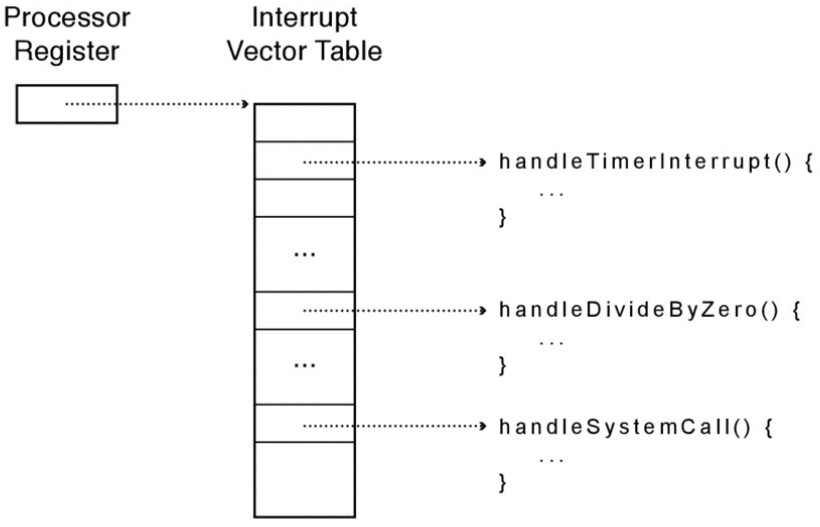
\includegraphics[scale=0.55]{img/fig0204}}
\caption{Tabla vectorial de interrupciones: se enumeran las rutinas del núcleo para manejar varias interrupciones de hardware, excepciones del procesador, y las llamadas al sistema.}
\label{fig0204}
\end{figure}

Como ilustra la \textit{Fig.} \ref{fig0204}, el procesador tiene un registro especial que apunta a un área de memoria del núcleo llamada la tabla vectorial de interrupciones. La tabla vectorial de interrupciones es una matriz de punteros, con cada entrada apuntando a la primera instrucción de un procedimiento controlador diferente en el núcleo. Un \textit{manejador de interrupciones} es el término usado para el procedimiento llamado por el núcleo en una interrupción.

El formato de la tabla vectorial de interrupciones es específico del procesador. En el x86, por ejemplo, las entradas $0-31$ de la tabla vectorial de interrupciones son para diferentes tipos de excepciones del procesador (por ejemplo, división por cero); las entradas $32-255$ son de diferentes tipos de interrupciones (temporizador, teclado, etc.); y, por convención, la entrada $64$ apunta al controlador de llamadas al sistema (\textit{trap}). El hardware determina qué dispositivo de hardware ha causado la interrupción, si la instrucción \textit{trap} fue ejecutada, o qué condición de excepción ocurrió. De este modo, el hardware puede seleccionar la entrada de la derecha de la tabla de interrupciones e invocar el manejador apropiado.

\subsection{Pila de Interrupciones}
En la mayoría de los procesadores, un registro de hardware especial con privilegios apunta a una región de la memoria del núcleo llamada pila de interrupción. Cuando una interrupción \textit{trap}, una excepción del procesador o llamada al sistema provoca un cambio de contexto en el núcleo, el hardware cambia el puntero de pila para que apunte a la base de la pila de interrupción del núcleo. El hardware guarda automáticamente algunos de los registros del proceso interrumpido agregándolos a la pila de interrupción antes de llamar al controlador del núcleo.

Cuando se ejecuta el controlador de kernel, agrega cualquier registro restante a la pila antes de realizar su trabajo. Al regresar de la interrupción, excepción del procesador o llamada al sistema, ocurre lo contrario: en primer lugar, el controlador quita de la pila los registros guardados y, a continuación, el hardware restaura los registros que guardó, volviendo al punto en que se interrumpió el proceso. Al regresar de una llamada al sistema, el valor del contador de programa guardado se debe incrementar de modo que el hardware vuelva a la instrucción que se encuentra inmediatamente después de la que causó la llamada a sistema.

Se necesita una pila de interrupción separada, con nivel kernel, por dos razones:

\begin{itemize}
\item \textbf{Confiabilidad}. Un puntero de pila a un proceso de nivel de usuario podría apuntar a una dirección de memoria no válida (por ejemplo, si el programa tiene un error), pero el controlador del núcleo debe seguir trabajando correctamente.

\item \textbf{Seguridad}. En un multiprocesador, otros subprocesos que se ejecutan en el mismo proceso pueden modificar la memoria del usuario durante una llamada al sistema. Si el controlador del núcleo almacena sus variables locales en la pila a nivel de usuario, el programa de usuario puede ser capaz de modificar la dirección de retorno del núcleo, potencialmente causando que el kernel salte a código arbitrario.
\end{itemize}

En un multiprocesador, cada procesador tiene que tener su propia pila de interrupción de modo que, por ejemplo, el núcleo pueda manejar llamadas simultáneas y excepciones del sistema a través de múltiples procesadores. Para cada procesador, el núcleo asigna una región separada de la memoria como pila de interrupción de dicho procesador.

\subsection{Dos Pilas por Proceso}
La mayoría de los kernels de sistemas operativos van un paso más allá y asignan una pila de interrupción del núcleo para cada proceso a nivel de usuario. Cuando un proceso a nivel de usuario se está ejecutando, la pila de interrupción de hardware apunta a la pila del núcleo de ese proceso. Debe notarse que cuando un proceso está funcionando a nivel de usuario, no se está ejecutando en el núcleo por lo que su pila del núcleo está vacía.

La asignación de la pila del nucleo por proceso hace que sea más fácil cambiar a un nuevo proceso dentro de un manejador de interrupciones o una llamada al sistema.

\begin{figure}[tbhp]
\centerline{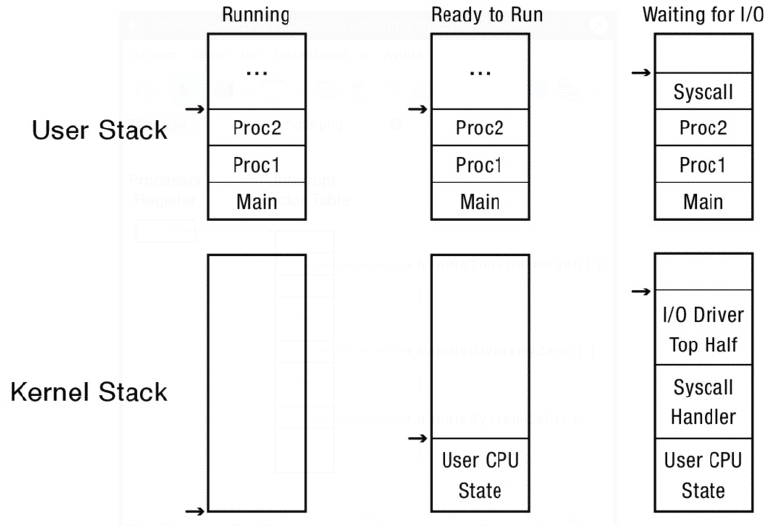
\includegraphics[scale=0.55]{img/fig0205}}
\caption{En la mayoría de sistemas operativos, un proceso tiene dos pilas: una para ejecutar código de usuario y una para el código del kernel.}
\label{fig0205}
\end{figure}

La \textit{Fig.} \ref{fig0205} resume los diversos estados de pilas de usuario y núcleo de un proceso:
\begin{itemize}
\item Si el proceso se está ejecutando en el procesador en modo de usuario, su pila del núcleo está vacía, lista para ser usada por una interrupción, excepción del procesador o llamada al sistema.

\item Si el proceso se está ejecutando en el procesador en modo de núcleo -- debido a una llamada de interrupción, excepción del procesador o llamada al sistema -- su pila de kernel está en uso, conteniendo los registros guardados de los cómputos en suspensión a nivel de usuario, así como el estado actual del controlador del kernel.

\item Si el proceso está disponible para funcionar, pero está esperando su turno en el procesador, la pila del núcleo contiene los registros y estado para ser restaurados cuando se reanude el proceso.

\item Si el proceso está esperando que se complete un evento de E/S, su pila del núcleo contiene el cómputo suspendido para ser reanudado cuando la E/S finaliza.
\end{itemize}

\subsection{El enmascaramiento de interrupciones}
Las interrupciones llegan de forma asíncrona; el procesador podría estar ejecutando un código usuario o un código del núcleo cuando llega una interrupción. El hardware provee de una instrucción con privilegios para aplazar temporalmente la entrega de una interrupción hasta que sea seguro hacerlo. En el {\mf x86} y varios otros procesadores, esta instrucción se llama \textit{deshabilitar interrupciones}. Sin embargo, la interrupción solo se aplaza (enmascarada), y no es ignorada. Una vez que se ejecuta la correspondiente instrucción \textit{habilitar interrupciones}, las interrupciones pendientes se entregan al procesador. Las instrucciones para enmascarar y desenmascarar interrupciones deben contar con privilegios, de lo contrario, un código de usuario podría inadvertidamente o maliciosamente desactivar el temporizador de hardware, permitiendo que la máquina se congele.

Si llegan múltiples interrupciones, mientras que las interrupciones están deshabilitadas, el hardware las enviará cuando se vuelvan a habilitar las interrupciones. Sin embargo, puesto que el hardware tiene búfer limitado para interrupciones pendientes, algunas interrupciones se podrían perder si están deshabilitadas por un período de tiempo demasiado largo. En general, el hardware retendrá una interrupción de cada tipo; el manejador de interrupciones es responsable de comprobar el hardware del dispositivo para ver si hay varios eventos de E/S pendientes que necesiten ser procesados.

Si el procesador recibe una interrupción en modo kernel con las interrupciones habilitadas, es seguro utilizar el puntero de pila actual en lugar de restablecerlo a la base de la pila de interrupción. Este enfoque puede agregar recursivamente una serie de estados de controladores sobre la pila. Entonces, cuando cada uno termina, su estado se saca de la pila, y el controlador anterior se reanuda donde quedó.

\subsection{Soporte de Hardware para el Ahorro y Restauración de Registros}
Los registros de un proceso interrumpido deben guardarse para que el proceso se pueda reiniciar exactamente donde se lo dejó. Debido a que el controlador puede cambiar los valores de los registros conforme se ejecuta, el estado debe guardarse antes de se ejecute el controlador. Debido a que la mayoría de las instrucciones modifican los contenidos de los registros, el hardware suele proporcionar instrucciones especiales para que sea más fácil de guardar y restaurar el estado de usuario.

Para hacer esto concreto, considérese la arquitectura {\mf x86}. En lugar de confiar en el software de controlador para hacer todo el trabajo, cuando se produce una interrupción o una \textit{trap}:
\begin{itemize}
\item Si el procesador está en modo de usuario, el {\mf x86} empuja el puntero de pila del proceso interrumpido en la pila de interrupción del núcleo y pasa a la pila del núcleo.

\item El {\mf x86} guarda el puntero de instrucción del proceso interrumpido.

\item El {\mf x86} guarda la \textit{palabra de estado} del procesador {\mf x86}. La palabra de estado del procesador incluye bits de control, tales como si la última operación aritmética en el código interrumpido resultó en un valor negativo, positivo o cero. Esto necesita ser guardado y restaurado para el comportamiento correcto de cualquier instrucción de salto condicional posterior.
\end{itemize}

El hardware guarda los valores para el puntero de pila, contador de programa y la palabra de estado del procesador antes de saltar a través de la tabla de vectores de interrupción al controlador de interrupciones. Una vez que el controlador se pone en marcha, estos valores serán las del controlador, no los del proceso interrumpido.

Una vez que el controlador se pone en marcha, se utilizan instrucciones especiales ({\mf PUSHAD} -- 32 bits y {\mf PUSHA} -- 16 bits) para guardar los registros restantes en la pila. Dado que el núcleo no suele realizar operaciones de punto flotante, éstos no necesitan ser guardados a menos que el kernel cambie a un proceso diferente.

La arquitectura {\mf x86} tiene características complementarias para la restauración de estado: una instrucción {\mf POPAD} para quitar un arreglo de registros de valores enteros de la pila y ponerlos en los registros; y {\mf iret} (regreso de interrupción), instrucción que carga un puntero de pila, puntero de instrucción, y la palabra de estado del procesador fuera de la pila en los registros del procesador apropiados.

\section{Poniendo todo junto: Modo de Transferencia x86}
Los pasos de alto nivel necesarios para manejar una interrupción, excepción del procesador o llamada al sistema son simples, pero los detalles requieren algún tipo de atención.

El {\mf x86} está segmentado, por lo que los punteros vienen en dos partes: $(i)$ un segmento, una región de memoria tal como código, datos, o la pila, y $(ii)$ un desplazamiento dentro de ese segmento. La instrucción actual a nivel de usuario es una combinación del segmento de código (registro {\mf CS}) más el puntero de instrucción (registro {\mf EIP}). Del mismo modo, la posición actual de la pila es la combinación de segmento de pila ({\mf SS}) y el puntero de pila dentro del segmento de pila ({\mf ESP}). El nivel de privilegio actual es almacenado como los bits de orden inferior del registro {\mf CS} en lugar de en la palabra de estado del procesador (registro {\mf eflags}). Los registros {\mf eflags} tienen códigos de condición que se modifican como un subproducto de la ejecución de las instrucciones; los registros {\mf eflags} también tienen otros indicadores que controlan el comportamiento del procesador, como por ejemplo cuando las interrupciones están enmascarados o no.

\begin{figure}[tbhp]
\centerline{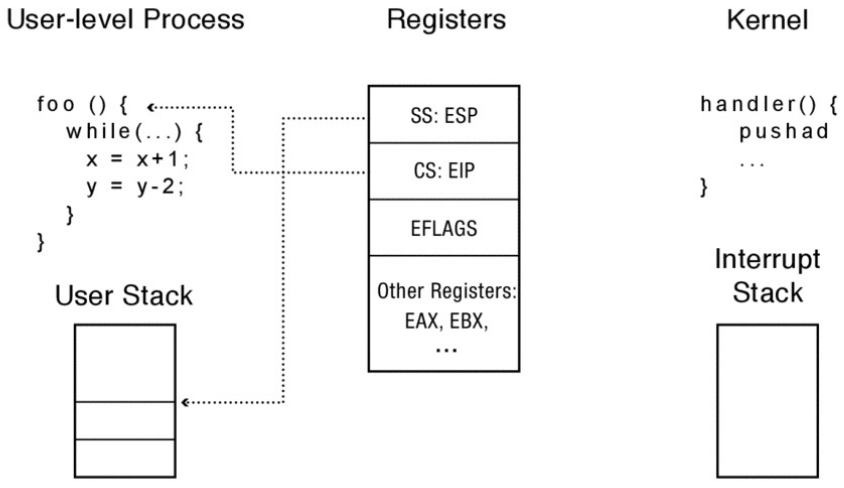
\includegraphics[scale=0.55]{img/fig0206}}
\caption{Estado del sistema antes de un manejador de interrupciones se invoca en la arquitectura {\mf x86}. {\mf SS} es el segmento de pila, {\mf ESP} es el puntero de pila, {\mf CS} es el segmento de código, y {\mf EIP} es el contador de programa. El contador de programa y puntero de pila se refiere a lugares en el proceso de usuario, y la pila de interrupción está vacía.}
\label{fig0206}
\end{figure}

Cuando un proceso a nivel de usuario está en ejecución, el estado actual del procesador, pila, la tabla vectorial de interrupciones del núcleo, y la pila del núcleo se ilustra en la \textit{Fig.} \ref{fig0206}. Cuando se produce una excepción del procesador o una llamada al sistema, el hardware guarda cuidadosamente una pequeña cantidad del estado del hilo interrumpido, que sale del sistema como se muestra en la \textit{Fig.} \ref{fig0207}:

\begin{figure}[tbhp]
\centerline{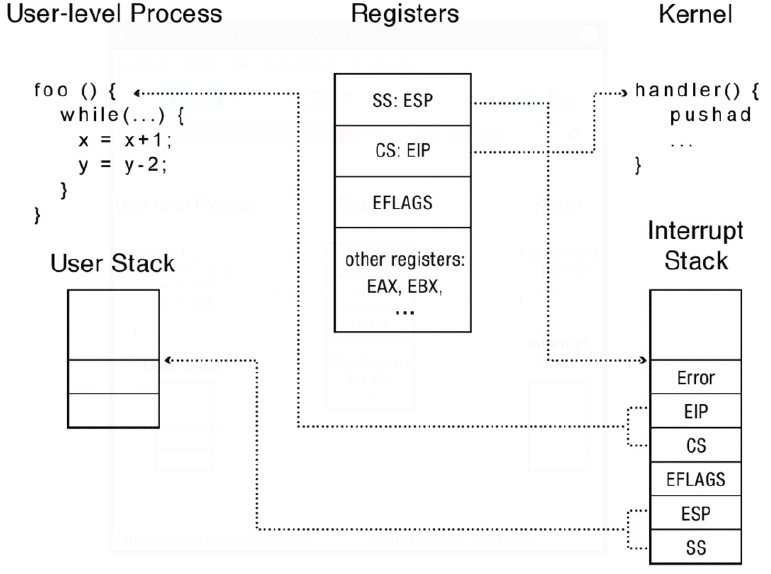
\includegraphics[scale=0.55]{img/fig0207}}
\caption{Estado del sistema después de que el hardware {\mf x86} ha saltado al manejador de interrupciones. El hardware guarda el contexto de usuario en la pila de interrupción del núcleo y cambia el contador de programa/pila a ubicaciones en la memoria del núcleo.}
\label{fig0207}
\end{figure}

\begin{enumerate}
\item \textbf{Enmascaramiento de interrupciones}. El hardware se inicia mediante la prevención de las interrupciones que se produzcan mientras el procesador está en el medio de cambiar de modo de usuario al modo kernel.

\item \textbf{Guardar tres valores clave}. El hardware guarda los valores del puntero de pila ({\mf ESP} y registros {\mf SS}), las banderas de ejecución (los registros {\mf eflags}), y el puntero de instrucción ({\mf EIP} y registros {\mf CS}) a los registros de hardware internos, temporales.

\item \textbf{Cambiar a la pila de interrupción del núcleo}. El hardware entonces cambia el puntero de pila/segmento de pila a la base de la pila de interrupción del núcleo, tal como se especifica en un registro especial de hardware.

\item \textbf{Guardar los tres valores clave en la nueva pila}. A continuación, el hardware almacena internamente los valores guardados en la pila.

\item \textbf{Opcionalmente guardar un código de error}. Ciertos tipos de excepciones, tales como fallos de página, generan un código de error que proporcionan más información sobre el evento. Para estas excepciones, el hardware guarda este código, dejándolo como primer elemento en la pila. Para otros tipos de eventos, el software del controlador de interrupción guarda un valor ficticio en la pila de forma que el formato de pila es idéntico en ambos casos.

\item \textbf{Invocar el manejador de interrupciones}. Por último, el hardware cambia el contador de código segmento/contador de programa a la dirección del procedimiento controlador de interrupciones. Un registro especial en el procesador contiene la ubicación de la tabla de vectores de interrupción en la memoria del núcleo. Este registro sólo puede ser modificada por el kernel. El tipo de interrupción se asigna a un índice de esta matriz, y el segmento de código/contador de programa se establece con el valor en este índice.
\end{enumerate}

Esto inicia el software de controlador.
El guía debe guardar primero el resto del estado del proceso interrumpido - que necesita para salvar a los otros registros antes de que los cambia! El controlador empuja el resto de los registros, incluyendo el puntero de pila actual, en la pila mediante la instrucción {\mf x86} \textit{PUSHAD}.

\begin{figure}[tbhp]
\centerline{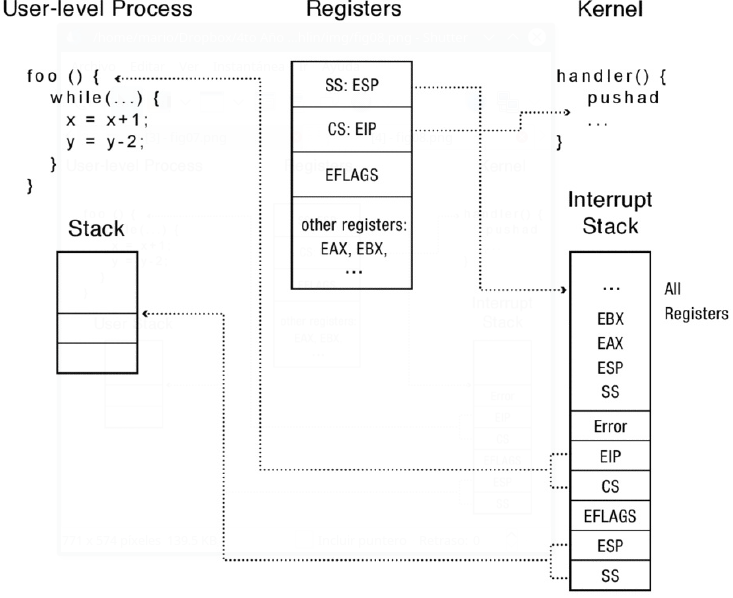
\includegraphics[scale=0.55]{img/fig0208}}
\caption{Estado del sistema después de que el controlador de interrupciones ha comenzado a ejecutar en la arquitectura {\mf x86}. El controlador guarda primero el estado actual de los registros del procesador, ya que puede sobrescribirlos. Nótese que esto guarda el puntero de pila dos veces: en primer lugar, el puntero a pila de usuario y a continuación, el puntero a pila del núcleo.}
\label{fig0208}
\end{figure}

Como muestra la \textit{Fig.} \ref{fig0208}, en este punto la pila de interrupción del núcleo posee $(1)$ el puntero de pila, banderas de ejecución, y el contador de programa guardados por el hardware, $(2)$ un código de error o valor ficticio, y $(3)$ una copia de todos los registros generales (incluyendo el puntero de pila, pero no el puntero de instrucción o los registros {\mf eflags}).

Una vez que el controlador ha guardado el estado del hilo interrumpido a la pila, puede utilizar los registros para lo que necesite, y puede guardar objetos adicionales en la pila. Por lo tanto, el controlador puede ahora hacer cualquier trabajo que tuviera por hacer.

Cuando el controlador finaliza, se puede reanudar el proceso interrumpido. Para ello, el controlador quita los registros guardados en la pila. Esto restaura todos los registros, excepto las banderas de ejecución, contador de programa, y puntero de pila. Para el conjunto de instrucciones {\mf x86}, la instrucción {\mf POPAD} se utiliza comúnmente. El controlador también quita el valor de error de la pila.

Por último, el controlador ejecuta la instrucción {\mf x86} \textit{iret} para restaurar el segmento de código, contador de programa, banderas de ejecución, segmento de pila, y el puntero a pila de la pila de interrupción del núcleo. Esto restaura el estado del proceso exactamente a como estaba antes de la interrupción. El proceso continúa la ejecución como si nada hubiera pasado.

Un pequeño pero importante detalle se produce cuando el hardware toma una excepción para emular una instrucción en el kernel, por ejemplo, por falta de hardware de punto flotante. Si el controlador vuelve de nuevo a la instrucción que provocó la excepción, otra excepción se repetiría al instante. Para evitar un bucle infinito, el gestor de excepciones modifica el contador de programa almacenado en la base de la pila para que apunte a la instrucción inmediatamente después de la causante de cambio de modo. La instrucción \textit{iret} luego puede volver al proceso de usuario en la ubicación correcta.

Para una llamada al sistema, el hardware {\mf x86} de Intel hace el incremento cuando se guarda el estado a nivel de usuario. El contador de programa para la instrucción después de la llamada al sistema se guarda en la pila de interrupción del núcleo.

\setcounter{subsection}{6}
\section{Inicio de un nuevo proceso}

Para empezar a correr a nivel de usuario el kernel debe:
\begin{itemize}
\item Asignar e inicializar el bloque de control de proceso.
\item Asignar memoria para el proceso.
\item Copie el programa del disco a la memoria recién asignada.
\item Asignar una pila de nivel de usuario para su ejecución a nivel de usuario.
\item Asignar una pila a nivel de kernel para el manejo de llamadas del sistema, interrupciones y excepciones del procesador.
\end{itemize}

Para iniciar la ejecución del programa, el núcleo también debe:
\begin{itemize}
\item \textbf{Copiar argumentos en la memoria de usuario}. Al iniciar un programa, el usuario puede darle argumentos, tanto como llamar a un procedimiento. Por ejemplo, cuando se hace clic en un icono de archivo en MacOS o Windows, el gestor de ventanas pide al kernel para iniciar la aplicación asociada con el archivo, pasándole el nombre de archivo que desea abrir. El kernel copia el nombre de archivo de la memoria del proceso del gestor de ventanas a una región especial de memoria en el nuevo proceso. Por convención, los argumentos a un proceso se copian en la base de la pila a nivel de usuario, y el puntero de pila del usuario se incrementa por lo que esas direcciones no se sobrescriben cuando el programa se pone en marcha.

\item \textbf{Transferir el control a modo de usuario}. Cuando se inicia un nuevo proceso, no existe un estado guardado para restaurar. Aunque sería posible escribir código especial para este caso, la mayoría de los sistemas operativos re-utilizan el mismo código para salir del núcleo, para iniciar un nuevo proceso y para el retorno de una llamada al sistema. Cuando creamos el nuevo proceso, asignamos una pila de kernel a la misma, y se reserva lugar en la parte inferior de la pila de kernel para los valores iniciales de sus registros de espacio de usuario, contador de programa, puntero de pila, y la palabra de estado del procesador. Para iniciar el nuevo programa, entonces podemos cambiar a la nueva pila y saltar a final del manejador de interrupciones. Cuando el controlador se ejecuta {\mf POPAD} y {\mf iret}, el procesador ``devuelve'' al inicio del programa de usuario.
\end{itemize}

Por último, aunque se puede pensar en un programa de usuario como a partir de una llamada principal (\textit{main}), de hecho, el compilador inserta un nivel de indirección. Se pone un trozo de programa en la ubicación de la memoria del proceso a la que el núcleo saltará cuando se inicia el proceso. El trabajo de este trozo es llamar al \textit{main} y luego, si éste retorna, llamar a salida -- la llamada al sistema para terminar el proceso. Sin este trozo, un programa de usuario que regresó del programa principal trataría de sacar de la pila el contador de programa de retorno, y puesto que no hay tal dirección en la pila, procesador comenzaría a ejecutar código aleatorio.

\chapter{La interfaz de programación}
Como se definió previamente, un proceso es una instancia de un programa -- el kernel proporciona un recinto de seguridad eficiente para ejecutar código no confiable a nivel de usuario, y ejecuta el código de usuario directamente en el procesador. Esta abstracción implica responder ``qué'' -- ¿qué funciones necesitamos que un sistema operativo proporcione a las aplicaciones?
\begin{itemize}
\item \textbf{Gestión de procesos}. ¿Puede un programa crear una instancia de otro programa? ¿Esperar a que éste se complete? ¿Detener o reanudar otro programa en ejecución? ¿Enviar un evento asíncrono?

\item \textbf{Entrada/Salida}. ¿Qué procesos se comunican con los dispositivos conectados al ordenador y a través de ellos con el mundo físico? ¿Pueden los procesos de comunicarse entre sí?

\item \textbf{Gestión de hilos}. ¿Podemos crear múltiples actividades o hilos que comparten memoria u otros recursos dentro de un proceso? ¿Podemos detener e iniciar los hilos? ¿Cómo sincronizar su uso de estructuras de datos compartidas?

\item \textbf{Gestión de la memoria}. ¿Puede un proceso de pedir más (o menos) espacio de memoria? ¿Puede compartir la misma región de memoria física con otros procesos?

\item \textbf{Sistemas de archivo y almacenamiento}. ¿Cómo un proceso almacena los datos del usuario de forma perdurable para que puedan sobrevivir si la máquina se cuelga o si falla el disco? ¿De qué manera el usuario da nombre y organiza sus datos?

\item \textbf{Redes y sistemas distribuidos}. ¿Qué procesos se comunican con los procesos de otros equipos? ¿De qué manera los procesos en diferentes equipos coordinan sus acciones a pesar de si la máquina se cuelga y hay problemas en la red?

\item \textbf{Gráficos y gestión de ventanas}. ¿Cómo un proceso controla un píxel en su porción de la pantalla? ¿Cómo un proceso hace uso de aceleradores gráficos?

\item \textbf{Autenticación y seguridad}. ¿Qué permisos tiene un usuario o un programa, y cómo estos permisos se mantienen actualizados? ¿En base a qué sabemos que el usuario (o programa) es quien dice ser?
\end{itemize}

\begin{figure}[tbhp]
\centerline{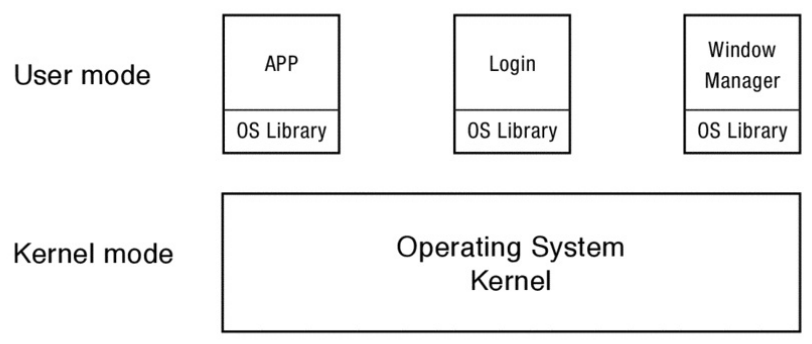
\includegraphics[scale=0.50]{img/fig0301}}
\caption{La funcionalidad del sistema operativo puede ser implementada en programas a nivel de usuario, en las bibliotecas a nivel de usuario, en el propio núcleo, o en un servidor de nivel de usuario invocado por el núcleo.}
\label{fig0301}
\end{figure}

En segundo lugar, tenemos que responder ``donde'' -- para cada bit de funcionalidad el sistema operativo proporciona programas de usuario; tenemos varias opciones para decidir, como se ilustra en la \textit{Fig.} \ref{fig0301}:

\begin{itemize}
\item Podemos poner la funcionalidad en un programa a nivel de usuario. En Windows y UNIX, por ejemplo, hay un programa de usuario para la gestión de inicio de sesión usuarios y otro para la gestión de los procesos de usuarios.

\item Podemos poner la funcionalidad de una biblioteca a nivel de usuario vinculados con cada aplicación. En Windows y MacOS, los \textit{widgets} de interfaz de usuario son parte de las bibliotecas a nivel de usuario, incluidas en aquellas aplicaciones que lo necesiten.

\item Podemos poner la funcionalidad en el núcleo del sistema operativo la cual se acceda través de una llamada al sistema. En Windows y UNIX, la gestión de procesos de bajo nivel, el sistema de archivos y la pila de red se implementan en el núcleo.

\item Podemos acceder a una funcionalidad a través de una llamada al sistema, pero la función podría implementarse en un proceso de servidor autónomo invocado por el núcleo. En muchos sistemas, el gestor de ventanas se implementa como un proceso de servidor independiente.
\end{itemize}

El sistema operativo proporciona la interfaz, donde cada función se implementa en base a un compromiso entre la \textit{flexibilidad}, \textit{fiabilidad}, \textit{rendimiento} y \textit{seguridad}.

\begin{itemize}
\item \textbf{Flexibilidad}. Es mucho más fácil cambiar el código del sistema operativo que vive fuera del núcleo, sin romper las aplicaciones que usan la interfaz antigua. Si creamos una nueva versión de una biblioteca, sólo podemos vincular esa biblioteca con nuevas aplicaciones, y con el tiempo convertir las aplicaciones antiguas para utilizar la nueva interfaz. Sin embargo, si hay que cambiar la interfaz de llamada al sistema, debemos o bien cambiar al mismo tiempo tanto el núcleo como todas las aplicaciones, o debemos seguir dando soporte a las versiones antigua y nueva hasta que todas las aplicaciones antiguas hayan sido convertidas. Muchas aplicaciones son escritas y desarrolladas por terceros, fuera del control del proveedor del sistema operativo. Por lo tanto, el cambio de la interfaz de llamada al sistema es un gran paso, que a menudo requiere la coordinación a través de muchas compañías.

\item \textbf{Seguridad}. Sin embargo, la gestión y protección de los recursos son responsabilidad del núcleo del sistema operativo. Los controles de protección no se pueden implementar en una biblioteca de nivel de usuario porque el código de aplicación puede saltarse todas las comprobaciones realizadas por la biblioteca.

\item \textbf{Confiabilidad}. La mejora de la fiabilidad es otra razón para mantener el núcleo del sistema operativo mínimo. El código del kernel necesita poder configurar los dispositivos de hardware, tales como el disco, y poder controlar los límites de protección entre aplicaciones. Sin embargo, los módulos del núcleo en general no se protegen entre sí, y un error en el código del kernel podría destruir datos de usuario o kernel. Esto ha llevado a algunos sistemas a utilizar una filosofía de ``lo que puede ser de nivel de usuario, debe serlo''. Una versión extrema de este enfoque consiste en aislar del resto del núcleo partes privilegiadas, pero menos críticas, del sistema operativo, como el sistema de archivos o el sistema de ventanas. Esto se conoce como diseño de \textbf{microkernel}. En un microkernel, el propio núcleo se mantiene pequeño, y en su lugar la mayor parte de la funcionalidad de un kernel de sistema operativo tradicional se pone en un conjunto de procesos de nivel de usuario, o servidores y se accede desde las aplicaciones de usuario a través de la comunicación entre procesos.

\item \textbf{Rendimiento}. Finalmente, transferir el control al núcleo es más costoso que una llamada de procedimiento a una biblioteca, y transferir el control a un servidor del sistema de archivos a nivel de usuario a través del kernel es aún más costoso. Los diseñadores de hardware han intentado reducir el costo de estos cruces fronterizos, pero su rendimiento sigue siendo un problema.
\end{itemize}

\section{Gestión de Procesos}
Hoy en día, los programas que crean y administran procesos incluyen administradores de ventanas, servidores web, navegadores web, intérpretes de línea de comandos de shell, etc. Si crear un proceso es algo que un proceso puede hacer, entonces cualquiera puede crear una nueva versión de cualquiera de estas aplicaciones, sin recompilar el kernel ni forzar a nadie a usarlo.

Una motivación temprana para la gestión de procesos a nivel de usuario era permitir a los desarrolladores escribir sus propios intérpretes de línea de comandos o \textit{shell}. Un \textit{shell} es un sistema de control de trabajos; Windows y UNIX tienen un \textit{shell}. Muchas tareas implican una secuencia de pasos para hacer algo, cada uno de los cuales puede ser su propio programa. Con un \textit{shell}, se puede escribir la secuencia de pasos, como una secuencia de programas para ejecutar cada paso. Por lo tanto, puede verlo como una versión muy temprana de un sistema de secuencias de comandos.

\subsection{Gestión de Procesos de Windows}
Un enfoque para la gestión de procesos es simplemente agregar una llamada al sistema para crear un proceso y otras llamadas a sistemas para otras operaciones de proceso. Esta resulta ser simple en teoría y compleja en la práctica. En Windows, hay una rutina llamada {\mf CreateProcess}.

Se llama al creador de procesos ``proceso padre'' y a los creados, ``procesos hijos''. ¿Qué pasos toma {\mf CreateProcess}? Como ya hemos explicado en el capítulo anterior, el núcleo necesita:

\begin{itemize}
\item Crear e inicializar el bloque de control de proceso (PCB) en el núcleo.
\item Crear e inicializar un nuevo espacio de direcciones.
\item Cargar el programa progresivo en el espacio de direcciones.
\item Copiar los argumentos {\mf args} en la memoria en el espacio de direcciones.
\item Inicializar el contexto de hardware para comenzar la ejecución en ``{\mf start}''.
\item Informar al programador que el nuevo proceso está listo para funcionar.
\end{itemize}

Por desgracia, hay algunos aspectos del proceso que el padre puede requerir controlar, tales como: sus privilegios, dónde enviar su entrada y salida, lo que debe almacenar en sus archivos, qué utilizar como una prioridad de planificación, etc. No podemos confiar en el proceso hijo para establecer sus propios privilegios y prioridad, y sería un inconveniente esperar que cada aplicación incluyera código para averiguar su contexto. Así que la interfaz real a {\mf CreateProcess} es bastante más complicada en la práctica

\subsection{Gestión de Procesos de UNIX}
UNIX tiene un enfoque diferente para el manejo de procesos, que es complejo en la teoría y simple en la práctica. UNIX divide en dos etapas a {\mf CreateProcess}, llamadas {\mf fork} y {\mf exec}, que se ilustra en la \textit{Fig.} \ref{fig0302}:
\begin{figure}[tbhp]
\centerline{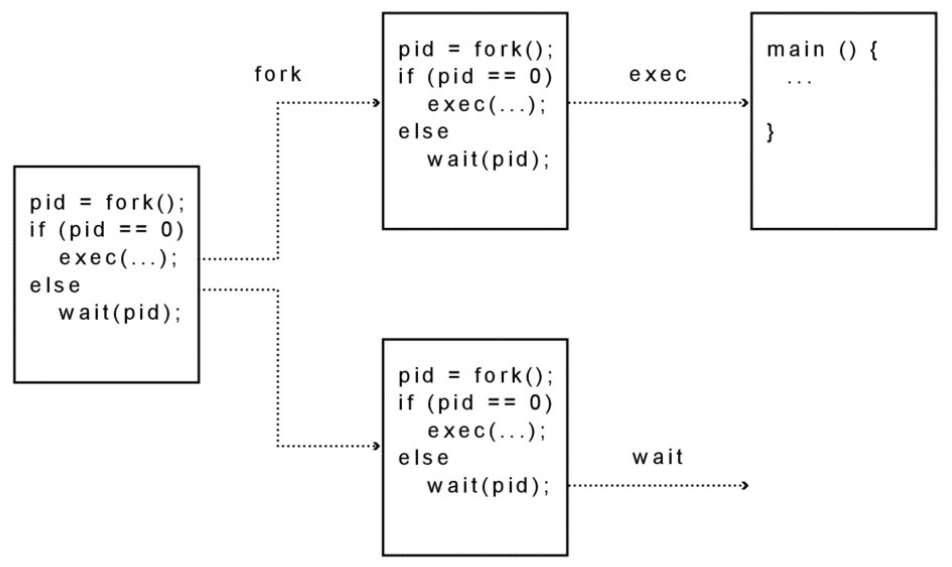
\includegraphics[scale=0.50]{img/fig0302}}
\caption{El funcionamiento de las llamadas {\mf fork} y {\mf exec}. {\mf fork} hace una copia del proceso padre; {\mf exec} cambia el proceso hijo para ejecutar el nuevo programa.}
\label{fig0302}
\end{figure}

El {\mf fork} de UNIX crea una copia completa del proceso padre, con una excepción clave (necesitamos una manera de distinguir cuál copia es el padre y cuál el hijo). El proceso hijo establece privilegios, prioridades, y E/S para el programa que está a punto de comenzar, por ejemplo, mediante el cierre de algunos archivos, la apertura de los demás, lo que reduce su prioridad si se va a ejecutar en segundo plano, etc. Debido a que el hijo corre exactamente el mismo código que el padre, se puede confiar en que va a establecer correctamente el contexto para el nuevo programa.

Una vez que se establece el contexto, el proceso hijo llama UNIX {\mf exec}. Esta llamada trae la nueva imagen ejecutable a la memoria y se pone en marcha. Puede parecer un desperdicio hacer una copia completa del proceso padre, sólo para sobrescribir esa copia cuando traemos en la nueva imagen ejecutable en la memoria usando {\mf exec}. Resulta que {\mf fork} y {\mf exec} se pueden implementar de manera eficiente.

Con este diseño, el {\mf fork} de UNIX no tiene argumentos y devuelve un entero. {\mf exec} toma dos argumentos (el nombre del programa a ejecutar y una serie de argumentos para transmitir al programa) -- en vez de los diez parámetros necesarios para {\mf CreateProcess}. En parte debido a la simplicidad de {\mf fork} y {\mf exec}, esta interfaz se ha mantenido prácticamente sin cambios desde que UNIX fue diseñado en la década de los '70. (Aunque la interfaz no ha cambiado, la palabra \textit{fork} es ahora un poco ambigua. Se utiliza para crear una nueva copia de un proceso, y en sistemas de hilos para crear un nuevo hilo. Para eliminar la ambigüedad, siempre vamos a utilizar el término ``{\mf fork} de UNIX'' ó ``UNIX {\mf fork}'' para referirnos a la llamada al sistema de proceso de copia de UNIX).

\textbf{UNIX {\mf fork}}

Los pasos para la implementación de {\mf fork} en el núcleo son:
\begin{itemize}
\item Crear e inicializar el bloque de control de proceso (PCB) en el núcleo.
\item Crear un nuevo espacio de direcciones.
\item Inicializar el espacio de direcciones con una copia de todo el contenido del espacio de direcciones de la matriz.
\item Heredar el contexto de ejecución de los padres (por ejemplo, todos los archivos abiertos).
\item Informar al programador que el nuevo proceso está listo para funcionar.
\end{itemize}

Un aspecto curioso del {\mf fork} es que la llamada al sistema devuelve dos valores: uno para el padre y uno para el hijo. Para el padre, UNIX devuelve el ID del proceso hijo; para el hijo, devuelve cero que indica el éxito. Del mismo modo que si ha creado un clon de sí mismo, lo que se necesita es alguna forma de saber quién era el clon y quien era el original, UNIX utiliza el valor de retorno de {\mf fork} para distinguir las dos copias.

\textbf{UNIX {\mf exec} y {\mf wait}}

La llamada al sistema {\mf exec} completa los pasos necesarios para iniciar la ejecución de un nuevo programa. El proceso hijo llama normalmente a {\mf exec} una vez que ha regresado del {\mf fork} y configurado el entorno de ejecución para el nuevo proceso. {\mf exec} realiza los siguientes pasos (tenga en cuenta que {\mf exec} no crea un nuevo proceso):
\begin{itemize}
\item Carga el programa {\mf prog} en el espacio de direcciones actual.
\item Copia los argumentos {\mf args} en el espacio de direcciones de la memoria.
\item Inicializa el contexto de hardware para comenzar la ejecución en ``inicio''.
\end{itemize}

Por otro lado, a menudo el proceso padre necesita hacer una pausa hasta que el proceso hijo haya terminado, por ejemplo, si el siguiente paso depende de la salida de la etapa anterior. UNIX tiene una llamada al sistema {\mf wait}, que detiene al padre hasta que el hijo finaliza, se rompe o es terminado. Dado que el padre podría haber creado muchos procesos hijos, {\mf wait} se parametriza con el ID de proceso del hijo.

Por último, UNIX proporciona la posibilidad de que un proceso pueda mandar a otro proceso una notificación instantánea o llamada ascendente. En UNIX, la notificación se realiza enviando una señal (\textit{signal}). Las señales se utilizan para terminar una aplicación, suspenderla temporalmente para depuración, reanudarla después de una suspensión, expirar el temporizador, y una serie de otras razones. Por lo general, si la aplicación receptora no especificó un manejador de señales, el núcleo implementa una estándar en su nombre.

\section{Estructura del Sistema Operativo}
Hay muchas dependencias entre los módulos dentro del sistema operativo, y a menudo hay una interacción bastante frecuente entre estos módulos:

\begin{itemize}
\item Muchas partes del sistema operativo dependen de primitivas de sincronización para coordinar el acceso a las estructuras de datos compartidas con el kernel.
\item El sistema de memoria virtual depende del soporte de hardware de bajo nivel para la traducción de direcciones, un soporte que es específico para una arquitectura de procesador en particular.
\item Tanto el sistema de archivos como el sistema de memoria virtual comparten una base común de bloques de memoria física. Ambos también dependen del controlador de dispositivo de disco.
\item El sistema de archivos puede depender de la pila de protocolos de red si el disco se encuentra físicamente en un equipo diferente.
\end{itemize}

Esto ha llevado a los diseñadores de sistemas operativos a luchar por lograr un compromiso fundamental: mediante la centralización de funciones en el kernel, se mejora el rendimiento y hace que sea más fácil de organizar una estrecha integración entre los módulos del núcleo. Sin embargo, los sistemas resultantes son menos flexibles, más difíciles de cambiar, y menos adaptables a las necesidades del usuario de la aplicación. Se discuten estos intercambios mediante la descripción de varias opciones para la arquitectura del sistema operativo.

\subsection{Núcleos monolíticos}
\begin{figure}[tbhp]
\centerline{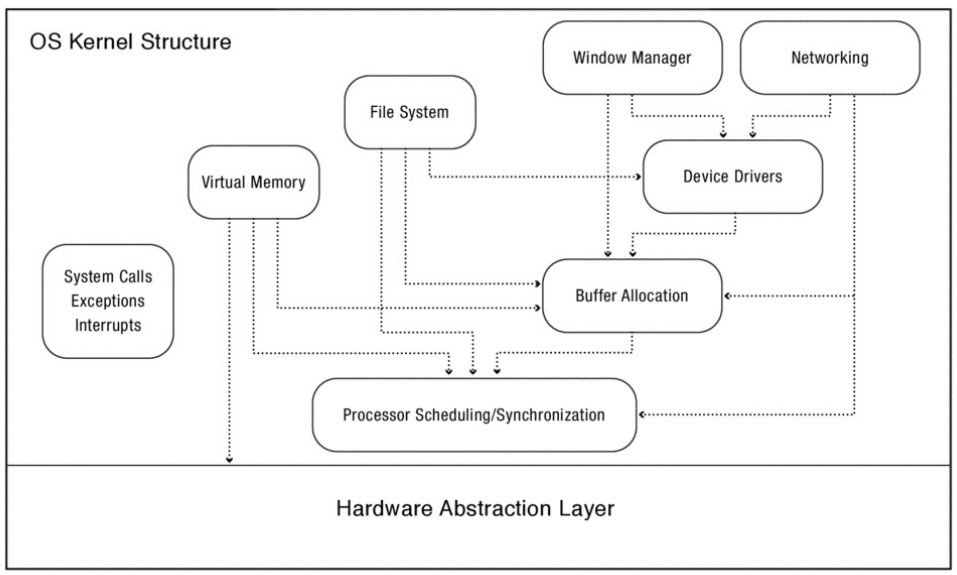
\includegraphics[scale=0.55]{img/fig0303}}
\caption{En el kernel de un sistema operativo monolítico, la mayor parte de la funcionalidad del sistema operativo está unida entre sí dentro del kernel. Los módulos del kernel llaman directamente a otros módulos del kernel para realizar las funciones necesarias. Por ejemplo, el sistema de memoria virtual utiliza gestión de memoria intermedia, la sincronización, y la capa de abstracción de hardware.}
\label{fig0303}
\end{figure}

Casi todos sistemas operativos comerciales ampliamente utilizados, como Windows, MacOS y Linux, pueden adoptar un enfoque similar al diseño monolítico de  la arquitectura del núcleo. Como se muestra en la \textit{Fig.} \ref{fig0303}, con un núcleo monolítico, la mayor parte de la funcionalidad del sistema operativo funciona en el interior del kernel del sistema operativo. En verdad, el término es un nombre poco apropiado, porque incluso en los llamados sistemas monolíticos, a menudo hay grandes segmentos que los usuarios consideran ``sistema operativo'' que se ejecuta fuera del kernel, ya en forma de utilidades como la \textit{shell}, o en las bibliotecas del sistema, tales como bibliotecas para gestionar la interfaz de usuario.

Dentro de un núcleo monolítico, el diseñador del sistema operativo es libre de desarrollar cualquier interfaz que cobre sentido entre los módulos, y por lo tanto hay un poco de variación entre diferentes sistemas operativos para esas estructuras internas. Sin embargo, para mejorar la portabilidad, dos temas son comunes en todos los sistemas: casi todos los sistemas operativos modernos tienen tanto una capa de abstracción de hardware y controladores de dispositivos de carga dinámica.

\textbf{Capa de Abstracción de Hardware}

Un objetivo clave de los sistemas operativos es ser portable a través de una amplia variedad de plataformas de hardware. Para lograr esto, especialmente dentro de un sistema monolítico, se requiere un diseño cuidadoso de la capa de abstracción de hardware. La capa de abstracción de hardware (HAL: \textit{\textit{Hardware Abstraction Layer}}) es una interfaz portátil de configuración de la máquina y operaciones específicas del procesador dentro del kernel. Por ejemplo, dentro de la misma familia de procesadores, tales como Intel {\mf x86}, diferentes fabricantes de ordenadores requerirán un código específico diferente del equipo para configurar y gestionar las interrupciones y temporizadores de hardware.

Los sistemas operativos que son portables a través de distintas familias de procesadores, por ejemplo entre un ARM y un sistema {\mf x86} o entre uno de 32 bits y uno de de 64 bits, necesitarán código específico del procesador para cambio de contexto entre procesos e hilos. El manejo de \textit{traps} de interrupciones, excepciones de procesador y llamadas al sistema es también específico del procesador; todos los sistemas tienen estas funciones, pero la aplicación concreta puede variar.

En cambio, con una capa de abstracción de hardware bien definida, la mayor parte del sistema operativo es independiente de la máquina y del procesador. Por lo tanto, portar un sistema operativo a un nuevo ordenador es sólo una cuestión de crear nuevas implementaciones de estas rutinas HAL de bajo nivel y re-vincular.

\textbf{Instalando dinámicamente los controladores de dispositivos}

Una consideración similar lleva a sistemas operativos que pueden acomodar fácilmente una amplia variedad de dispositivos físicos de E/S. Aunque hoy día sólo hay un puñado de diferentes conjuntos de instrucciones de arquitectura ampliamente usados, hay un gran número de diferentes tipos de dispositivos físicos de E/S, fabricados por un gran número de empresas. Hay diversidad en las interfaces de hardware para los dispositivos, así como en los conjuntos de chips de hardware para la gestión de los dispositivos.

Para mantener la portabilidad del kernel del sistema operativo, queremos desacoplar el código fuente del sistema operativo de los aspectos específicos de cada dispositivo. La innovación clave, ampliamente adoptada hoy, es un controlador de dispositivo de carga dinámica. Un \textbf{controlador de dispositivo de carga dinámica} (\textit{dinamically loadable device driver}) es un software para gestionar un dispositivo específico, interfaz o conjunto de chips, agregado al kernel del sistema operativo después de que el kernel comienza a funcionar, para manejar los dispositivos que están presentes en una máquina en particular. El fabricante del dispositivo normalmente proporciona el código del controlador, utilizando una interfaz estándar soportada por el kernel. El kernel del sistema operativo llama al controlador cada vez que necesita leer o escribir datos en el dispositivo.

El sistema operativo se carga (\textit{bootea}) con un pequeño número de controladores de dispositivos -- por ejemplo, uno para el disco (para leer los binarios del sistema operativo en la memoria). Para los dispositivos conectados físicamente al equipo, el fabricante del equipo reúne los controladores o \textit{drivers} en un archivo que almacena junto con el gestor de arranque. Cuando el sistema operativo se inicia, consulta en el bus de E/S los dispositivos que están conectados a la computadora y luego carga los controladores del archivo en el disco. Por último, para cualquier dispositivo conectado a la red, tal como una impresora de red, el sistema operativo puede cargar los \textit{drivers} a través de Internet.

Mientras que los \textit{drivers} de dispositivo se pueden cargar dinámicamente para resolver un problema, suponen uno diferente. Los errores en un controlador de dispositivo pueden corromper las estructuras del kernel del sistema operativo y datos de aplicación; al igual que con un programa regular, los errores no pueden ser atrapados de inmediato, de modo que el usuario puede no ser consciente de que sus datos están siendo modificados silenciosamente. Lo que es peor, un atacante malintencionado puede utilizar controladores de dispositivo para introducir un virus informático en el núcleo del sistema operativo, y por lo tanto obtener el control de todo el equipo.

Los desarrolladores de sistemas operativos han llevado a cabo cinco enfoques para hacer frente a este problema:

\begin{itemize}
\item \textbf{Inspección de código}. Proveedores de sistemas operativos suelen requerir todo el código de controlador de dispositivo sea sometido a inspecciones y pruebas, antes de introducirse en el núcleo.
\item \textbf{Seguimiento de errores}. Después de cada caída del sistema, el sistema operativo puede recopilar información acerca de la configuración del sistema y de la pila del kernel actual, y enviar esta información a una base de datos central para su análisis. Muchos accidentes ocurren dentro del controlador de dispositivo en sí, pero incluso aquellos que no lo hacen a veces pueden ser localizados. Por ejemplo, si los fallos se correlacionan con la presencia de un controlador de dispositivo en particular, o aumentan después del lanzamiento de una nueva versión del controlador, esto podría indicar el origen del problema.
\item \textbf{Controladores de dispositivos a nivel de usuario}. Tanto Apple como Microsoft estimulan fuertemente nuevos controladores de dispositivos que funcionen a nivel de usuario en lugar de en el núcleo. Cada controlador de dispositivo se ejecuta en un proceso independiente a nivel de usuario y mediante llamadas al sistema se puede manipular el dispositivo físico. De esta manera, un driver sólo puede afectar a sus propias estructuras de datos internos y no el resto del núcleo del sistema operativo. Si el driver de dispositivo se bloquea, el núcleo puede reiniciarlo fácilmente.
\item \textbf{Controladores de dispositivo de máquina virtual}. Para manejar los controladores de dispositivos heredados, un enfoque que ha ganado algo de terreno es ejecutar el código del controlador de dispositivo dentro de un sistema operativo invitado (\textit{guest}) que se ejecuta en una máquina virtual. El sistema operativo invitado carga los controladores de dispositivo como si se estuviese ejecutando directamente en el hardware real, pero cuando los dispositivos intentan acceder al hardware físico, el monitor de máquina virtual subyacente recupera el control para garantizar la seguridad. Los controladores de dispositivos todavía pueden tener errores, pero sólo pueden dañar el sistema operativo invitado y no otras aplicaciones que se ejecutan en el monitor de máquina virtual subyacente.

\item \textbf{Controlador Sandboxing}. Otro desafío tanto para controladores de dispositivos a nivel de usuario como para controladores de máquina virtual es el rendimiento. Algunos controladores de dispositivos necesitan una interacción frecuente con el hardware y el resto del núcleo. Algunos investigadores han propuesto ejecutar los controladores de dispositivo en su propio entorno de ejecución restringido en el interior del núcleo. Esto requiere técnicas livianas de \textit{sandboxing} (aislamiento de procesos).
\end{itemize}

\subsection{MicroKernels}
Una alternativa al enfoque núcleo monolítico es ejecutar tantas partes del sistema operativo como sea posible en uno o más servidores de nivel de usuario. El gestor de ventanas en la mayoría de los sistemas operativos funciona de esta manera: aplicaciones individuales dibujan cosas en su porción de la pantalla mediante el envío de peticiones al gestor de ventanas. El gestor de ventanas decide la ventana de qué aplicación está delante o detrás para cada píxel de la pantalla, y luego \textit{renderiza} el resultado. Si el sistema tiene un hardware acelerador de gráficos presente, el administrador de ventanas puede usarlo para procesar elementos más rápidamente. Algunos sistemas han trasladado otras partes del sistema operativo a servidores de nivel de usuario: la pila de red, el sistema de archivos, drivers de dispositivos, etc.

La diferencia entre diseños microkernel y monolítico con frecuencia es transparente para el programador de la aplicación. La ubicación del servicio puede estar oculta en una biblioteca de nivel de usuario - las llamadas van a la biblioteca, la cual arroja solicitudes ya sea como llamadas al sistema o como leer y escribir en el servidor a través de una tubería (\textit{pipe}). La ubicación del servidor también se puede ocultar en el interior del núcleo - la aplicación llama al núcleo como si el núcleo implementara el servicio, pero en su lugar el núcleo cambia el formato de la solicitud en una tubería que el servidor puede leer.

Un diseño de microkernel ofrece un beneficio considerable para el desarrollador del sistema operativo, ya que es más fácil de modularizar y cuenta con servicios de depuración a nivel de usuario. Aparte de una potencial de mejora de la fiabilidad, sin embargo, los microkernels ofrecen poco beneficio visible a los usuarios finales y puede ralentizar el rendimiento general mediante la inserción de pasos adicionales entre la aplicación y los servicios que necesita. Por lo tanto, en la práctica, la mayoría de los sistemas adoptan un modelo híbrido en el que algunos servicios del sistema operativo se ejecutan a nivel de usuario y algunos están en el núcleo, en función de la solución de compromiso entre la complejidad del código específico y el rendimiento.

\chapter{Concurrencia e Hilos}
En el mundo real - fuera de las computadoras - diferentes actividades con frecuencia ocurren al mismo tiempo. Usamos la palabra \textit{Concurrencia} para referirnos a múltiples actividades que pueden ocurrir al mismo tiempo. El mundo real es concurrente, e internamente, las computadoras modernas también son concurrentes. Por ejemplo, un servidor de alta gama puede tener más de una docena de procesadores, 10 discos y 4 interfaces de red; una estación de trabajo podría tener una docena de dispositivos de E/S activos que incluyen una pantalla, teclado, ratón, cámara, micrófono, altavoz, interfaz de red inalámbrica, cable de interfaz de red, una impresora, un escáner, y la unidad de disco. Hoy en día, incluso los teléfonos móviles suelen tener procesadores de múltiples núcleos.

La correcta gestión de la concurrencia es un desafío clave para los desarrolladores de sistemas operativos. Para gestionar los recursos de hardware, para proporcionar la capacidad de respuesta a los usuarios, y para ejecutar varias aplicaciones al mismo tiempo, el sistema operativo necesita una forma estructurada de hacer el seguimiento de las diversas acciones que necesita realizar. Veremos un conjunto de abstracciones para expresar y gestionar la concurrencia. Estas abstracciones son de uso generalizado en los sistemas operativos comerciales, ya que reducen la complejidad de implementación, mejoran la fiabilidad del sistema y mejoran el rendimiento.

La concurrencia también es una preocupación para muchos desarrolladores de aplicaciones. A pesar de que las abstracciones ya discutidas fueran desarrolladas originalmente para que sea más fácil escribir código correcto del sistema operativo, éstas han llegado a ser ampliamente utilizadas en aplicaciones:
\begin{itemize}
\item Los servicios de red necesitan ser capaces de manejar múltiples peticiones de sus clientes; un Google que maneje sólo una solicitud de búsqueda a la vez, o un Amazon que sólo permita que se compre un libro a la vez, serían mucho menos útil.
\item La mayoría de las aplicaciones de hoy en día tienen interfaces de usuario. Proporcionar una buena capacidad de respuesta a los usuarios, realizando al mismo tiempo la lógica de aplicación es mucho más fácil con un enfoque estructurado para la concurrencia.
\item Programas paralelos tienen que ser capaces de mapear el trabajo en múltiples procesadores para obtener los beneficios de rendimiento de las arquitecturas multikernel.
\item Sistemas de gestión de datos necesitan de la concurrencia para enmascarar la latencia de las operaciones de disco y de red.
\end{itemize}

Desde la perspectiva del programador, es mucho más fácil pensar secuencialmente que realizar el seguimiento de las muchas actividades simultáneas. Por ejemplo, al leer o escribir el código de un procedimiento, se puede identificar un estado inicial y un conjunto de condiciones previas, pensar en cómo cada declaración sucesiva cambia el estado, y desde ahí determinar las condiciones posteriores.

El sistema operativo proporciona la ilusión de que los programadores pueden crear tantos hilos, como necesiten, y cada hilo se ejecuta en su propio procesador virtual dedicado. En realidad, por supuesto, una máquina sólo tiene un número finito de procesadores, y es el trabajo del sistema operativo, de forma transparente, multiplexar los hilos en los procesadores actuales.

La idea clave es escribir un programa simultáneo -- uno con muchas actividades simultáneas -- como un conjunto de flujos secuenciales de ejecución, o \textit{hilos}, que interactúan y comparten los resultados de maneras muy precisas. Se define un conjunto de tareas que se ejecutan concurrentemente mientras que el código para cada tarea es secuencial. Cada hilo se comporta como si tuviera su propio procesador dedicado. Como veremos más adelante, utilizando la abstracción de hilo a menudo se requiere que el programador escriba código adicional para la coordinación de múltiples hilos con el acceso a estructuras de datos compartidas.

La abstracción de hilo permite al programador crear tantos procesos como sea necesario, sin tener que preocuparse por el número exacto de procesadores físicos, o exactamente qué procesador va a trabajar en cada instante. Por supuesto, los hilos son solamente una abstracción: el hardware físico tiene un número limitado de procesadores (y potencialmente único). El trabajo del sistema operativo es el de proporcionar la ilusión de un número casi infinito de procesadores virtuales. Se sostiene esta ilusión mediante la suspensión y reanudación de hilos de modo que en cualquier momento dado sólo un subconjunto de los hilos se estén ejecutando activamente de manera transparente.

\section{Casos de uso de los Hilos}
La intuición detrás de la abstracción de hilo es simple: en un programa, podemos representar cada tarea concurrente como un hilo. Cada hilo proporciona la abstracción de ejecución secuencial similar al modelo de programación tradicional. De hecho, podemos pensar en un programa tradicional como un único subproceso con una secuencia lógica de pasos que cada instrucción sigue a la anterior. El programa ejecuta sentencias, itera a través de bucles y llamadas/retornos de procedimientos, uno tras otro.

Un programa multi-hilo es una generalización del mismo modelo de programación básica. A cada hilo individual le sigue una secuencia de pasos que ejecuta sentencias, itera a través de bucles, llamadas/retornos de procedimientos, etc. Sin embargo, un programa puede disponer de varios hilos que se ejecutan al mismo tiempo.

\subsection{Cuatro razones para usar Hilos}
El uso de hilos para expresar y gestionar la concurrencia tiene varias ventajas:
\begin{itemize}
\item \textbf{Estructura del programa: expresar lógicamente tareas concurrentes}. Los programas a menudo interactúan o simulan aplicaciones del mundo real que tienen actividades concurrentes. Los hilos le permiten expresar la concurrencia natural de una aplicación escribiendo cada tarea concurrente como un hilo separado. Por ejemplo, para obtener la entrada del ratón y al mismo tiempo volver a dibujar la pantalla y enviar y recibir paquetes desde la red, los procesadores físicos tienen que dividir su tiempo entre estas tareas.

\item \textbf{Capacidad de respuesta: el cambio de trabajo se ejecuta en segundo plano}. Para mejorar la respuesta al usuario y el rendimiento, un patrón de diseño común es crear hilos para realizar un trabajo en segundo plano, sin que el usuario esté esperando el resultado. De esta manera, la interfaz de usuario puede permanecer sensible a otros comandos, independientemente de la complejidad de la petición del usuario. En un navegador web, por ejemplo, el botón de cancelación debe continuar trabajando incluso si la página es gigantesca o una secuencia de comandos en la página tarda mucho tiempo para ejecutarse.

Muchas aplicaciones tienen un bucle: obtener una orden del usuario, a continuación, ejecutar el comando, a continuación, obtener el siguiente comando. Sin embargo, si algunos comandos toman mucho tiempo para llevarse a cabo, una aplicación que se ejecuta secuencialmente no será capaz de comprobar la siguiente operación hasta que la anterior esté completa. Para mantener la interfaz de respuesta, podemos utilizar hilos para dividir cada comando en dos partes: cualquier cosa que se puede hacer al instante se puede hacer en el bucle de eventos principal, y en un hilo separado podemos realizar el resto de las tareas en segundo plano.

\item \textbf{Rendimiento: aprovechando múltiples procesadores}. Los programas pueden utilizar hilos en un multiprocesador que hace el trabajo en paralelo; pueden hacer el mismo trabajo en menos tiempo o más trabajo en el mismo tiempo transcurrido. Hoy en día, un servidor puede tener más de una docena de procesadores; una computadora de escritorio o portátil pueden incluir ocho núcleos de procesador; incluso la mayoría de los teléfonos inteligentes son máquinas multinúcleo. Una ventaja de utilizar hilos para el paralelismo es que el número de hilos no tiene por qué coincidir exactamente con el número de procesadores del hardware en el que se está ejecutando. El sistema operativo de manera transparente maneja decide qué hilos se ejecutan en qué procesadores y en qué momento.

\item \textbf{Rendimiento: gestión de los dispositivos de E/S}. Para hacer un trabajo útil, los equipos deben interactuar con el mundo exterior a través de los dispositivos de E/S. Mediante la ejecución de tareas como hilos separados, cuando una tarea está a la espera de E/S, el procesador puede avanzar en una tarea diferente.

El beneficio de la concurrencia entre el procesador y la E/S es doble: en primer lugar, los procesadores son a menudo mucho más rápidos que los sistemas de E/S con los que interactúan, por lo que mantener la inactividad del procesador durante la E/S desperdiciaría gran parte de su capacidad. Por ejemplo, la latencia para leer desde el disco puede ser de decenas de milisegundos, lo suficiente para ejecutar más de 10 millones de instrucciones en un procesador moderno. Después de solicitar un bloque de disco, el sistema operativo puede cambiar a otro programa, o de otro hilo dentro del mismo programa, hasta que el disco haya finalizado y el hilo original esté listo para reanudar.

En segundo lugar, la E/S proporciona una forma para que la computadora interactué con entidades externas, como cuando los usuarios presionan teclas de un teclado o un equipo remoto que envía paquetes de red. La llegada de este tipo de eventos de E/S es impredecible, por lo que el procesador debe ser capaz de trabajar en otras tareas mientras sigue respondiendo rápidamente a estos eventos externos.
\end{itemize}

\section{La abstracción Hilo}
Hasta el momento, hemos descrito lo que un hilo es y por qué es útil. Antes de ir más lejos, hay que definir la abstracción hilo y sus propiedades con mayor precisión. Un hilo es una única secuencia de ejecución que representa una tarea planificable por separado.

\begin{itemize}
\item  \textbf{Secuencia de ejecución única}. Cada hilo ejecuta una secuencia de instrucciones -- asignaciones, condicionales, bucles, procedimientos, y así sucesivamente -- al igual que en el modelo de programación secuencial.
\item \textbf{Tarea planificable por separado}. El sistema operativo puede ejecutar, suspender o reanudar un hilo en cualquier momento.
\end{itemize}

\subsection{Ejecución, Suspensión y Reanudación de Hilos}
Los hilos proporcionan la ilusión de un número infinito de procesadores. Para ello el sistema operativo debe ejecutar las instrucciones de cada hilo de manera que cada uno progrese. Pero el hardware subyacente tiene sólo un número limitado de procesadores, y quizás único. Para asignar a un conjunto arbitrario de hilos a un conjunto fijo de procesadores, los sistemas operativos incluyen un programador de subprocesos que puede cambiar entre los hilos que se están ejecutando y los que están listos pero no en ejecución. El cambio entre hilos es transparente para el código que está siendo ejecutado dentro de cada hilo. La abstracción hace que cada hilo parezca ser un único flujo de ejecución; esto significa que el programador puede prestar atención a la secuencia de la instrucción dentro o fuera de un hilo o cuando esa secuencia puede ser (temporalmente) suspendida para permitir la ejecución de otro hilo.

Por lo tanto, los hilos proporcionan un modelo de ejecución en el que cada hilo se ejecuta en un procesador virtual dedicado a una velocidad impredecible y variable. Desde el punto de vista del código de un hilo, cada instrucción aparece para ser ejecutada inmediatamente después de la anterior. Sin embargo, el planificador puede suspender a un hilo entre una instrucción y la siguiente y volver a correrlo más tarde. Es como si el hilo se ejecuta en un procesador que a veces se vuelve muy lento.

\begin{figure}[tbhp]
\centerline{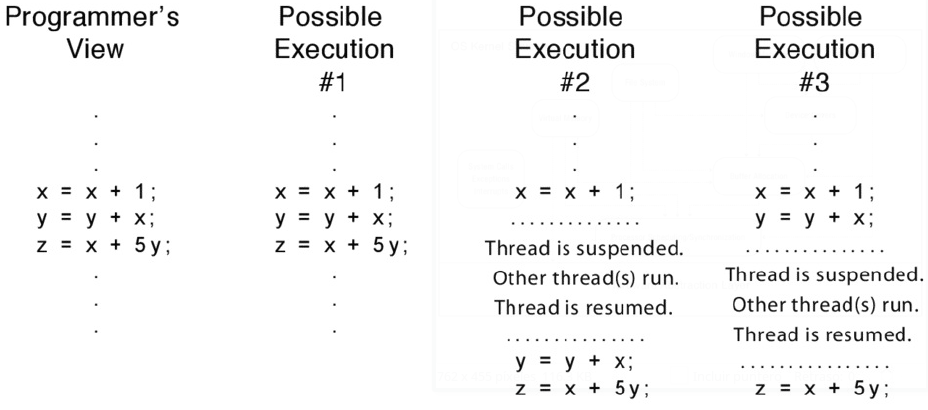
\includegraphics[scale=0.50]{img/fig0401}}
\caption{Tres posibles formas en que un hilo puede ejecutar, todas cuales son equivalentes a la vista del programador}.
\label{fig0401}
\end{figure}

La \textit{Fig.} \ref{fig0401} ilustra la vista del programador de un programa sencillo y tres (de muchas) maneras posibles de cómo el programa puede ser ejecutado, dependiendo de lo que haga el planificador. Desde el punto de vista del hilo, o de la velocidad de ejecución, las alternativas son equivalentes. De hecho, el hilo típicamente no es consciente de cuál de estos (u otros) se produce en realidad durante la ejecución.

\begin{figure}[tbhp]
\centerline{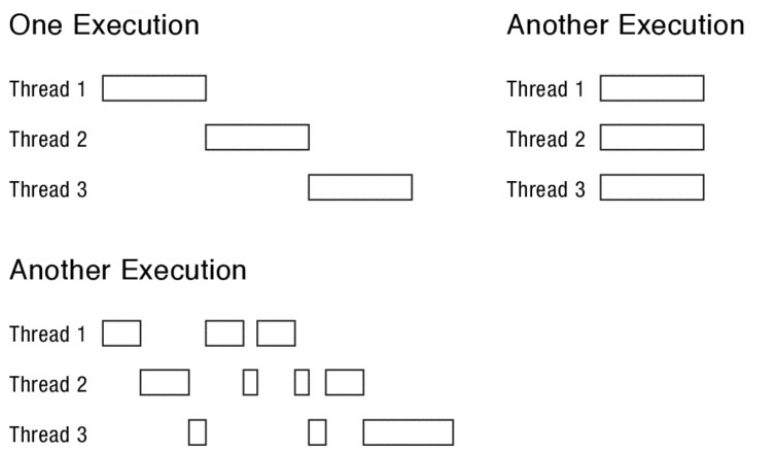
\includegraphics[scale=0.55]{img/fig0402}}
\caption{Algunas de las muchas maneras posibles que tres hilos podrían ser intercalados en tiempo de ejecución.}
\label{fig0402}
\end{figure}

¿Cómo se programan los hilos afecta a la intercalación de un hilo con otros hilos. La \textit{fug.} \ref{fig0402} muestra algunas de las muchas posibles intercalaciones de un programa con tres hilos. El programador de hilos, por tanto, no debe hacer ninguna suposición sobre la velocidad relativa con la que ejecutan diferentes hilos.

\subsection{Por qué la Velocidad Variable?}
Puede parecer extraño requerir a los programadores suponer que el procesador virtual de un hilo corre a una velocidad impredecible y que cualquier intercalación con otros hilos es posible. Sin duda, el programador debe ser capaz de aprovechar el hecho de que algunos intercalados son más propensos que otros?

El modelo de programación con hilos adopta esta suposición como una forma de guiar a los programadores al razonar sobre la exactitud. En lugar de asumir que un hilo corre a la misma velocidad que los otros (o más rápido o más lento) y tratar de escribir programas que coordinen los hilos sobre la base de su velocidad relativa de ejecución, los programas multihilo debiesen no hacer suposiciones sobre el comportamiento del planificador de hilos. A su vez, las decisiones de planificación del kernel -- cuándo asignar un hilo a un procesador y cuándo adelantarse a un subproceso diferente -- se puede hacer sin tener que preocuparse de si podría afectar a la exactitud del programa o no.

Si los hilos son completamente independientes entre sí, sin compartir memoria u otros recursos, entonces la orden de ejecución no importa -- cualquier momento producirá el mismo resultado que cualquier otro. La mayoría de los programas multihilo comparten estructuras de datos, sin embargo, el programador debe utilizar la sincronización explícita para garantizar la exactitud del programa, independientemente de la posible intercalación de instrucciones de diferentes hilos.

Incluso podríamos pasar por alto el tema de la planificación -- por ejemplo, si hay más procesadores que hilos de manera que a cada hilo se le asigne su propio procesador físico -- la realidad física es que la velocidad de ejecución relativa de los diferentes hilos puede verse afectada significativamente por factores fuera de su control. Un ejemplo extremo es que el programador puede estar depurando un hilo paso a paso, mientras que otros hilos corren a toda velocidad en otros procesadores. Si el programador ha de tener alguna esperanza de entender el comportamiento concurrente del programa, la exactitud éste no puede depender de qué hilos están siendo observados.

La variabilidad en la velocidad de ejecución se produce también durante el funcionamiento normal. El acceso a memoria puede estancar un procesador para cientos o miles de ciclos si se produce un \textit{fallo de caché}. Otros factores incluyen la frecuencia con la que el programador tiene prioridad sobre el hilo, el número de procesadores físicos que están presentes en una máquina, el tamaño de las cachés, qué tan rápida es la memoria, cómo el firmware de ahorro de energía se ajusta la velocidad de reloj de los procesadores, los mensajes que llegan la red, o lo que se recibe de entrada del usuario. Las velocidades de ejecución de los diferentes hilos de un programa son difíciles de predecir, puede variar en un hardware diferente, e incluso puede variar de una ejecución a otra en el mismo hardware. Como resultado, hay que coordinar las acciones de hilo a través de la sincronización explícita en lugar de tratar de razonar acerca de su velocidad relativa.

\section{API de Hilos Simples}
Una buena manera de entender la API de hilos simples es que proporciona una manera de invocar una llamada asíncrona a procedimiento. Una llamada de procedimiento normal pasa a un conjunto de parámetros a la función, la función se ejecuta inmediatamente en la pila del llamador, y cuando se termina la función, el control vuelve de nuevo al llamador con el resultado. Una llamada asíncrona a procedimiento separa la llamada de la devolución: con {\mf thread\_create}, el llamador inicia la función, pero a diferencia de una llamada a procedimiento normal, el llamador continúa la ejecución concurrente con la función llamada. Más tarde, el llamador puede esperar a la finalización de función (con {\mf thread\_join}).

La función {\mf thread\_create} es análoga a los procesos {\mf fork} y {\mf exec} de UNIX, mientras {\mf thread\_join} es análoga al proceso de UNIX {\mf wait}. UNIX {\mf fork} crea un nuevo proceso que se ejecuta simultáneamente con el proceso que llama a {\mf fork}; UNIX {\mf exec} hace que ese proceso ejecute un programa específico. UNIX {\mf wait} permite que la llamada a proceso suspenda la ejecución hasta la finalización del nuevo proceso.

\subsection{Paralelismo fork-join}
Muchas aplicaciones multihilo pueden diseñarse utilizando sólo estas operaciones de hilo y ninguna sincronización adicional. Con paralelismo {\mf fork-join}, un hilo puede crear hilos hijos para realizar el trabajo ({\mf fork} o {\mf thread\_create}), y se puede esperar sus resultados ({\mf join}). Los datos pueden ser compartidos de forma segura entre los hilos, siempre que $(a)$ sean escritos por el padre antes de que el hilo hijo inicie o $(b)$ sean escritos por el hijo y leído por el padre después de {\mf join}.

Si se siguen estas restricciones al compartir, cada hilo se ejecuta de forma independiente y de una manera determinista, no siendo afectado por el comportamiento de cualquier otro hilo que se ejecute simultáneamente. La multiplexación de hilos en procesadores no tiene otro efecto que el rendimiento.

\section{Estructura de Datos y Ciclo de Vida de un Hilo}
Como hemos visto, cada hilo representa un flujo secuencial de ejecución. El sistema operativo proporciona la ilusión de que cada hilo se ejecuta en su propio procesador virtual mediante la suspensión y reanudación de los hilos de forma transparente. Para que la ilusión funcione, el sistema operativo debe guardar con precisión y restaurar el estado de un hilo. Sin embargo, debido a que los hilos funcionan tanto en un proceso o en el núcleo, también hay un estado \textit{compartido} que no se guarda o se restaura cuando se cambia el procesador entre los hilos.

Por lo tanto, para entender cómo el sistema operativo implementa la abstracción hilo, hay que definir tanto el estado de cada subproceso y el estado que se comparte entre los hilos. Entonces podemos describir el ciclo de vida de un hilo -- cómo el sistema operativo puede crear, iniciar, detener y eliminar hilos para proporcionar la abstracción.

\subsection{Bloque de Control de un Hilo y sus Estados - TCB}
El sistema operativo necesita una estructura de datos para representar el estado de un hilo; un hilo es como cualquier otro objeto en este sentido. Esta estructura de datos se llama el \textbf{bloque de control de hilo} (TCB). Para cada hilo que crea el sistema operativo, se crea una TCB. El bloque de control del hilo mantiene dos tipos de información para cada subproceso:
\begin{enumerate}
\item El estado de la computación que se realiza por el hilo.
\item Los metadatos sobre el hilo que se utilizan para gestionar el hilo.
\end{enumerate}

\textbf{Cálculo del Estado para cada subproceso}. Para crear múltiples hilos y ser capaz de iniciar y detener cada hilo, según sea necesario, el sistema operativo debe asignar espacio en el TCB para el estado actual de la ejecución de cada hilo: un puntero a la pila del subproceso y una copia de sus registros del procesador.

\begin{itemize}
\item \textbf{Pila}. La pila de un hilo es la misma que la pila para un cómputo con un solo hilo: almacena la información necesaria para los procedimientos anidados que el hilo está ejecutando actualmente. Por ejemplo, si un hilo llama {\mf foo()}, {\mf foo()} llama a {\mf bar()}, y el {\mf bar()} llama a {\mf bas()}, entonces la pila contendría una estructura de pila para cada uno de estos tres procedimientos; cada estructura de pila contiene las variables locales utilizadas por el procedimiento, los parámetros del procedimiento que se llamó, y la dirección de retorno a la que deberá saltar a cuando finaliza el procedimiento.

Debido a que en un momento dado diferentes hilos pueden estar en difer-entes estados en sus cálculos secuenciales -- cada uno puede estar en un lugar diferente en un procedimiento distinto llamado con diferentes argumentos de un agrupamiento diferente de los procedimientos que encierra -- cada hilo necesita su propia pila. Cuando se crea un nuevo hilo, el sistema operativo asigna una nueva pila y almacena un puntero a la pila en el TCB.

\item \textbf{Copia de los registros del procesador}. Los registros del procesador incluyen no sólo sus registros de propósito general para el almacenamiento de valores intermedios para los cálculos actuales, sino que también incluyen los registros de propósito especial, como el puntero de instrucción y puntero de pila.

Para poder suspender un hilo, ejecutar otro hilo, y luego reanudar el hilo original, el sistema operativo necesita un lugar para almacenar los registros de un hilo cuando el hilo no se está ejecutando de forma activa. En algunos sistemas, los registros de propósito general para un hilo detenido se almacenan en la parte superior de la pila, y la TCB incluye solamente un puntero a la pila. En otros sistemas, el TCB contiene espacio para una copia de todos los registros del procesador.
\end{itemize}

\textbf{Los metadatos para cada subproceso}. El TCB también incluye metadatos para cada subproceso -- información para la gestión del hilo. Por ejemplo, cada hilo podría tener un ID de hilo, la prioridad en la planificación y el estado (por ejemplo, si el hilo está esperando un evento o está listo para ser colocado en un procesador).

\subsection{Estados Compartidos}
A diferencia del estado por hilo que se asigna para cada hilo, algún estado se comparte entre los hilos que se ejecutan en el mismo proceso o dentro del núcleo del sistema operativo. En particular, el código de programa es compartido por todos los hilos en un proceso, aunque cada hilo puede estar ejecutándose en un lugar diferente dentro de ese código. Además, las variables globales asignadas estáticamente y las variables de almacenadas dinámicamente en heap pueden contener información accesible para todos los subprocesos.

ADVERTENCIA: Aunque existe una división lógica importante entre el estado por hilo y estado compartido, el sistema operativo normalmente no hace cumplir esta división. Nada impide que un hilo con errores acceda al estado de un hilo (conceptualmente privado) de otro hilo. Escribir mal un puntero a un hilo puede corromper la pila de otro hilo. O un programador descuidado podría pasar un puntero a una variable local en la pila de un hilo a otro hilo, dando al segundo hilo un puntero a una ubicación de pila cuyo contenido puede cambiar a medida que se ejecutan las primeras llamadas y retornos de diversos procedimientos. O el primer hilo puede salir después de la entrega de un puntero a una variable en su pila; el heap reasignará la memoria a un fin distinto. Debido a que estos errores pueden depender de las intercalaciones específicas de las ejecuciones de los hilos, pueden ser extremadamente difíciles de localizar y corregir.

Para evitar comportamientos inesperados, es importante a la hora de escribir programas multihilo saber qué variables están diseñadas para ser compartidas a través de hilos (variables globales, objetos en la pila) y cuáles están diseñadas para ser privadas (variables locales/automáticas).

\section{Ciclo de Vida de un Hilo}
Es útil considerar la progresión de estados como un hilo va desde ser creado, hasta ser planificado y des-planificado dentro y fuera de un procesador, y luego a salir. La \textit{Fig.} \ref{fig0403} muestra los estados de un hilo durante su vida útil.
\begin{figure}[tbhp]
\centerline{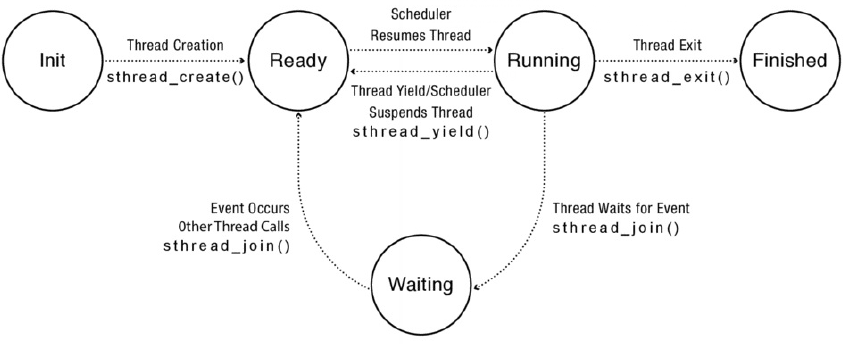
\includegraphics[scale=0.50]{img/fig0403}}
\caption{Los estados de un hilo durante su vida útil.}
\label{fig0403}
\end{figure}

\textbf{INIT (Inicio)}. La creación del hilo lo pone en su estado INIT y asigna e inicializa las estructuras de datos por hilo. Una vez hecho esto, el código de la creación del hilo pone al hilo en el estado READY mediante la adición del hilo a la READY LIST. Esta lista es el conjunto de hilos ejecutables que están esperando su turno para utilizar un procesador. En la práctica, la READY LIST no es en realidad una \textit{lista}; el sistema operativo utiliza típicamente una estructura de datos más sofisticada para realizar un seguimiento de hilos ejecutables, tales como una cola de prioridad. Sin embargo, vamos a referirnos a ella como la READY LIST.

\textbf{READY (Listo)}. Un hilo en el estado READY está disponible para ser ejecutado pero en la actualidad no se está ejecutando. Su TCB está en la READY LIST, y los valores de sus registros se almacenan en su TCB. En cualquier momento, el planificador puede lograr que un hilo haga la transición de READY a RUNNING copiando sus valores de registro de su TCB a los registros de un procesador.

\textbf{RUNNING (En Ejecución)}. Un hilo en estado de RUNNING se esta ejecutando en un procesador. En este momento, sus valores de registro se almacenan en el procesador en vez de en el TCB. Un hilo en estado RUNNING puede pasar al estado READY de dos maneras:
\begin{itemize}
\item El planificador puede adelantar un hilo en RUNNING y moverlo al estado READY por: $(1)$ guardar los registros del hilo en su TCB y $(2)$ cambiar al procesador para ejecutar el siguiente hilo en la READY LIST.
\item Un hilo en estado RUNNING puede renunciar voluntariamente al procesador y pasar de RUNNING a READY por una llamada (por ejemplo, {\mf thread\_yield} en la biblioteca del hilo).
\end{itemize}

Observe que un hilo puede pasar de READY a RUNNING y volver muchas veces. Dado que el sistema operativo guarda y restaura exactamente los registros de cada hilo, sólo la velocidad de ejecución del hilo se ve afectada por estas transiciones.

\textbf{WAITING (En Espera)}. Un hilo en el estado de WAITING está a la espera de algún acontecimiento. Mientras que el planificador puede mover un hilo en el estado READY al estado de RUNNING, un hilo en el estado de WAITING no se puede ejecutar hasta que alguna acción de otro hilo lo mueva de WAITING a READY.

Mientras el hilo espera por un evento, no puede progresar, por lo tanto, no es útil ejecutarlo. En lugar de seguir ejecutando el hilo o guardar la TCB en la READY LIST del planificador, la TCB se almacena en la lista de espera (WAITING LIST) de alguna \textit{variable de sincronización} asociada al evento. Cuando se produce el evento requerido, el sistema operativo mueve la TCB de la lista de espera de la variable de sincronización a la READY LIST del planificador, efectuándose la transición en el hilo de estado WAITING a READY.

\textbf{FINISHED (Terminado)}. Un hilo en estado FINISHED nunca se ejecuta de nuevo. El sistema puede liberar parte o la totalidad de su estado para otros usos, aunque puede mantener algunos remanentes del hilo en la fase de producto terminado por un tiempo poniendo la TCB en una FINISHED LIST. Por ejemplo, la llamada {\mf thread\_exit} permite a un hilo pasar su valor de salida a su padre a través del hilo {\mf thread\_join}. Finalmente, cuando el estado de un hilo ya no es necesario (por ejemplo, después de que su valor de salida ha sido leído por la llamada a {\mf join}), el sistema puede eliminar y recuperar el estado del hilo.

\section{Implementacion de Hilos en el Kernel}
Hasta ahora, hemos descrito las estructuras de datos básicos y el funcionamiento de un hilo. A continuación se describe cómo ponerlos en práctica. Los detalles de la aplicación varían en función del contexto:
\begin{itemize}
\item \textbf{Los hilos del núcleo}. La forma más simple de implementar hilos es en el interior del núcleo del sistema operativo, compartiendo uno o más procesadores físicos. Un hilo del núcleo ejecuta el código del núcleo y modifica las estructuras de datos del núcleo. Casi todos los sistemas operativos hoy en día soportan hilos en su núcleo.

\item \textbf{Los hilos del núcleo y los procesos de un único hilo}. Un sistema operativo con hilos del núcleo también puede ejecutar algunos procesos de usuario de un único subproceso. Estos procesos pueden invocar llamadas al sistema que se ejecutan al mismo tiempo que los hilos del núcleo en el interior del núcleo.

\item \textbf{Los procesos multihilos que utilizan los hilos del núcleo}. La mayoría de los sistemas operativos proporcionan un conjunto de rutinas y bibliotecas de sistema para permitir a las aplicaciones utilizar múltiples hilos dentro de un solo proceso a nivel de usuario. Estos hilos ejecutan código de usuario y tienen estructuras de datos de acceso a nivel de usuario. También hacen llamadas al sistema en el núcleo del sistema operativo. Para ello, necesitan una pila de interrupciones del núcleo al igual que un proceso normal de un solo hilo.

\item \textbf{Hilos a nivel de usuario}. Para evitar tener que hacer una llamada al sistema para cada operación, algunos sistemas soportan un modelo en el que las operaciones de hilos a nivel de usuario -- crear, entregar, unir, salir, y las rutinas de sincronización -- son implementadas en su totalidad a nivel de usuario, sin necesidad de invocar al núcleo.
\end{itemize}

\subsection{Creación de un Hilo}
Hay tres pasos para crear un hilo:
\begin{enumerate}
\item \textbf{Asignarle un estado al hilo}. El primer paso en el constructor del hilo es asignar espacio para el estado por hilo: la TCB y la pila. Como hemos mencionado, la TCB es la estructura de datos del sistema de hilos utiliza para manejar el hilo. La pila es un área de memoria para almacenar datos acerca de los procedimientos en progreso; se guardará en memoria como cualquier otra estructura de datos.

\item \textbf{Inicializar el estado por hilo}. Para inicializar el TCB, el constructor establece los registros de los nuevos hilos que se van a necesitar cuando el hilo se ponga en RUNNING. Cuando al hilo se le asigna un procesador, queremos que comience a correr {\mf func(arg)}. Sin embargo, en lugar de tener el inicio de hilo en {\mf func}, el constructor inicia el hilo en una función ficticia, \textit{stub}, que a su vez llama {\mf func}.

\item \textbf{Poner la TCB en la READY LIST}. El último paso en la creación de un hilo es para establecer su estado a READY y poner el nuevo TCB en la READY LIST, lo que permite que el hilo ingrese al planificador.
\end{enumerate}

\subsection{Eliminación de un Hilo}
Cuando un hilo llama {\mf thread\_exit}, hay dos pasos para borrar el hilo:
\begin{itemize}
\item Retirar el hilo de la READY LIST de modo que nunca se ejecute de nuevo.
\item Liberar el estado por hilo asignado para el hilo.
\end{itemize}

Aunque esto parece fácil, hay una sutileza importante: si un hilo se elimina en sí de la READY LIST y libera su propio estado por hilo, entonces el programa podría romperse. Por ejemplo, si un hilo se remueve a sí mismo de la READY LIST, pero se produce una interrupción antes de que el hilo acabe des-asignar su estado, lo que produce una pérdida de memoria: el hilo no se reanudará a des-asignar su estado.

Peor aún, supongamos que un hilo libera su propio estado. ¿Puede el hilo terminar de ejecutar el código en {\mf thread\_exit} si no tiene una pila? ¿Qué ocurre si se produce una interrupción justo después de la pila del hilo se ha des-asigna? Si el código de cambio de contexto intenta guardar el estado del hilo actual, se va a escribir en memoria des-asignada, posiblemente ya utilizada para almacenamiento por otro procesador que ha asignado alguna otra estructura de datos. El resultado podría ser memoria dañada, donde el comportamiento específico depende de la secuencia precisa de los eventos. No hace falta decir que un error de este tipo sería muy difícil de localizar.

Afortunadamente, hay una solución sencilla: un hilo no elimina su propio estado. En su lugar, algún otro flujo debe hacerlo. Al salir, las transiciones del hilo al estado FINISHED mueven su TCB de la READY LIST a una lista de hilos terminados que el planificador no debe correr nunca. El hilo puede cambiar de forma segura al siguiente hilo en la READY LIST. Una vez que el hilo terminado ya no está en funcionamiento, es seguro que \textit{algún otro} flujo libere el estado del hilo.

\subsection{Cambio de contexto para un hilo}
Para dar soporte a múltiples hilos, también necesitamos un mecanismo para cambiar entre hilos en estado READY y RUNNING.

Un cambio de contexto suspende la ejecución de un hilo actualmente en ejecución y reanuda la ejecución de algún otro hilo. El SWITCH guarda los registros del hilo que se está ejecutando actualmente, la TCB y la pila del hilo, y luego se restauran los registros del nuevo hilo, su TCB y la pila, en el procesador. A continuación se da respuesta a varios interrogantes asociados a este tema.

\textbf{¿Qué desencadena un cambio de contexto de un hilo del núcleo?} Un cambio de contexto puede ser desencadenado por una llamada ya sea voluntaria en la biblioteca de hilo, o una interrupción involuntaria o excepción de procesador.
\begin{itemize}
\item \textbf{Voluntario}. El hilo podría llamar a una función de biblioteca de hilo que desencadene un cambio de contexto. Por ejemplo, la mayoría de las bibliotecas de hilos proporcionan una llamada {\mf thread\_yield} que permite que el hilo que se está ejecutando actualmente entregue voluntariamente el procesador al siguiente hilo en la READY LIST. Del mismo modo, los {\mf thread\_join} y {\mf thread\_exit} suspenden la ejecución del hilo actual y empiezan a correr uno diferente.

\item \textbf{Involuntario}. Una interrupción o una excepción de procesador podría invocar un controlador de interrupciones. El hardware de interrupción guarda el estado del hilo en ejecución y ejecuta el código del controlador. El controlador puede decidir que algún otro hilo se debe ejecutar, y luego cambiar a él. Alternativamente, si el hilo actual debería continuar funcionando, el controlador restablece el estado del hilo interrumpido y reanuda la ejecución.

Por ejemplo, muchos sistemas de hilos están diseñados para asegurar que ningún hilo pueda monopolizar el procesador. Para lograr esto, se dispuso un temporizador de hardware para interrumpir el procesador periódicamente (por ejemplo, cada pocos milisegundos). El manejador de interrupción de temporizador guarda el estado del hilo en ejecución, escoge otro hilo para ejecutar, y se ejecuta ese hilo mediante la restauración de su estado anterior.

Otros eventos de hardware de E/S (por ejemplo, se pulsa una tecla del teclado, llega un paquete de red, o se completa una operación de disco) también invocan el manejador de interrupciones. En estos casos, así, los controladores guardan el estado del hilo actualmente en ejecución para que pueda ser restaurado más tarde. A continuación, se ejecuta el código del controlador, y cuando el controlador finaliza, o bien restaura el estado del hilo actual, o bien cambia a un nuevo hilo. Un nuevo hilo se ejecutará si el evento de E/S mueve un hilo a la READY LIST con una prioridad más alta que el hilo anteriormente en funcionamiento.
\end{itemize}

Independientemente de esto, el sistema de hilos debe guardar el estado actual del procesador, de modo que cuando el hilo actual reanuda la ejecución, parezca como si el evento nunca ocurrió excepto por haber transcurrido algo de tiempo. Esto proporciona la abstracción de la ejecución del hilo en un procesador virtual con velocidad impredecible y variable.

Para simplificar las cosas, no queremos hacer un cambio de contexto involuntario mientras estamos en medio de uno voluntario. Al cambiar entre dos hilos, es necesario aplazar temporalmente interrupciones hasta que el cambio se haya completado, para evitar confusiones. Los procesadores contienen instrucciones privilegiadas para diferir y volver a habilitar las interrupciones.

\textbf{Cambio de Contexto Voluntario de un hilo del núcleo}. Un hilo llama {\mf thread\_yield} para renunciar voluntariamente al procesador y dar lugar a otro hilo. Los registros del hilo se copian en su TCB y pila, y su reanudación se hará cuando el planificador lo elija.

La llamada {\mf thread\_yield} convierte primero las interrupciones para evitar que el sistema de hilos intente hacer dos cambios de contexto al mismo tiempo. A continuación, extrae el siguiente hilo para funcionar fuera de la READY LIST (si hay alguno), y cambia a éste.

El código de {\mf thread\_switch} se llama en el contexto del hilo anterior y termina en el contexto del nuevo hilo. Para que esto funcione, {\mf thread\_switch} guarda el estado de los registros en la pila y guarda el puntero de pila sobre la TCB. A continuación, pasa a la pila del nuevo hilo, restaura el estado del nuevo hilo de la pila de éste, y devuelve a cualquier contador de programa que se encuentre almacenado en la nueva pila.

\textbf{Cambio Involuntario de Contexto en el núcleo}. Al producirse una interrupción, una excepción, o una \textit{trap} interrumpe un proceso en ejecución a nivel de usuario, el hardware y el software funcionan juntos para guardar el estado del proceso interrumpido, ejecutar el controlador del núcleo, y restaurar el estado del proceso interrumpido.

El mecanismo es casi idéntico cuando una interrupción o una \textit{trap} desencadena un cambio de hilo entre hilos en el núcleo. Se producen los siguientes pasos:
\begin{enumerate}
\item \textbf{Guardar el estado}. Se guardan los registros del hilo actualmente en ejecución por lo que el controlador puede ejecutar código sin interrumpir el hilo. El hardware guarda algo del estado cuando se produce la interrupción o excepción, y el software guarda el resto del estado cuando el controlador se ejecuta.

\item \textbf{Ejecutar el controlador del núcleo}. Se ejecuta el código del controlador del núcleo para manejar la interrupción o excepción. Desde ya estamos en modo kernel, no es necesario cambiar de usuario al modo kernel en este paso. Asimismo, no hay que cambiar el puntero de pila a la base de la pila de interrupción del núcleo. En cambio, podemos simplemente empujar variables de estado o de controlador guardados en la pila actual, a partir del puntero de pila actual.

\item \textbf{Restaurar el estado}. Se restauran los registros del \textit{siguiente hilo listo} de modo que el hilo puede reanudar la ejecución en que se detuvo.
\end{enumerate}

En resumen, comparando un cambio entre los hilos del núcleo a lo que ocurre en una transferencia en modo de usuario: $(1)$ no hay necesidad de cambiar los modos (y por lo tanto no hay necesidad de cambiar las pilas) y $(2)$ el controlador puede reanudar cualquier hilo de la READY LIST en lugar de siempre reanudar el hilo o proceso que se acaba de suspender.

\textbf{Detalles de implementacion}. En la mayoría de las arquitecturas de procesador, una forma sencilla (pero ineficiente) para intercambiar al siguiente hilo desde el interior de un manejador de interrupciones es llamar a {\mf thread\_switch} justo antes de que el controlador retorne. Como ya hemos visto, {\mf thread\_switch} guarda el estado del hilo actual (es decir, el estado del controlador de interrupción) y cambia al nuevo hilo del núcleo. Cuando se reanuda el hilo original, volverá a partir {\mf thread\_switch}, y saca de inmediato de la pila el contexto de interrupción guardado, reanudando ejecución en el punto en que se interrumpió.

La mayoría de los sistemas, como Linux, hacen una pequeña optimización para mejorar el rendimiento de manejo de interrupciones. El estado del hilo interrumpido ya está guardado en la pila, aunque sea en el formato especificado por la interrupción de hardware. Si modificamos {\mf thread\_switch} para guardar y restaurar los registros exactamente de la misma forma que lo hace una interrupción de hardware, luego volver de una interrupción y reanudar un hilo son la misma acción: ambos quitan de la pila la estructura de interrupción para reanudar el siguiente hilo a ejecutar.

\section{Combinando hilos del Núcleo y procesos de usuario de hilo único}
Un proceso es una ejecución secuencial de instrucciones, por lo que cada proceso a nivel de usuario incluye el hilo del proceso. Sin embargo, un proceso es algo más que un hilo porque tiene su propio espacio de direcciones.

Debido a que un proceso contiene más que sólo un hilo, el bloque de control de proceso de cada proceso (PCB) necesita más información que un bloque de control de hilo (TCB) para un hilo del núcleo. Al igual que un TCB, una PCB para un proceso de un solo hilo debe almacenar los registros del procesador cuando el hilo del proceso no esté en ejecución. Además, el PCB tiene información sobre el espacio de direcciones del proceso; cuando se produce un cambio de contexto de un proceso a otro, el sistema operativo debe cambiar los mapeos de memoria virtual, así como el estado de registro.

Dado que la PCB y TCB representan cada uno un hilo, la READY LIST del núcleo puede contener una mezcla de PCB para los procesos y TCB para los hilos del núcleo. Cuando el planificador elige el siguiente hilo para ejecutar, se puede escoger uno u otro tipo. Un cambio de hilo es casi idéntico si se cambia entre los hilos del núcleo o la conmutación entre el hilo de un proceso y un hilo del núcleo. En ambos casos, el cambio guarda el estado del hilo que se está ejecutando actualmente y restaura el estado del siguiente hilo a ejecutar.

La mayoría de los sistemas operativos dedican una pila de interrupción del kernel para cada proceso. De esta manera, cuando el proceso tiene que realizar una llamada al sistema, o una interrupción o una excepción de procesador, el hardware atrapa estas interrupciones hacia el kernel, guarda el estado del procesador a nivel de usuario, y se pone en marcha en un controlador específico en el núcleo. Una vez dentro del núcleo, el hilo de proceso se comporta exactamente igual que un hilo del núcleo -- puede crear hilos (u otros procesos), bloquearse (por ejemplo, en UNIX {\mf wait } o en un evento de E/S), y hasta salir. Mientras tanto en el interior del núcleo, el proceso puede ser adelantado por una interrupción de temporizador o eventos de E/S, y un proceso de mayor prioridad o hilo del núcleo puede ejecutarse en su lugar. El PCB y la pila del núcleo para los procesos adelantados almacenan tanto el estado actual del núcleo, así como el estado de nivel de usuario guardado cuando el proceso inició la llamada al sistema.

Podemos reanudar un proceso en el núcleo usando {\mf thread\_switch}. Sin embargo, cuando reanudamos la ejecución del proceso a nivel de usuario después de la finalización de una llamada al sistema o interrupción, debemos restaurar su estado precisamente a como estaba antes: el valor correcto en sus registros, ejecutándose en modo usuario, con los mapeos  de memoria virtual apropiados, etcétera.

\section{Implementación de Procesos Multihilo}
Hasta ahora, hemos descrito cómo implementar varios hilos que se ejecutan en el interior del núcleo del sistema operativo. Por supuesto, también queremos ser capaces de ejecutar programas de usuario.

\subsection{Implementación de procesos multihilo que hacen uso de los hilos del kernel}
La forma más sencilla para soportar múltiples hilos por proceso es utilizar la APP hilo del núcleo que ya hemos descrito. Cuando un hilo del núcleo crea, elimina, suspende o reanuda otro hilo, se puede utilizar una simple llamada de procedimiento. Cuando un hilo a nivel de usuario accede a la biblioteca de hilo para hacer las mismas cosas, se utiliza una llamada al sistema para pedir al kernel que haga la operación en su nombre.

Un hilo en un proceso tiene:
\begin{itemize}
\item Una pila de nivel de usuario para ejecutar código de usuario.
\item Una pila de interrupción del núcleo para cuando este hilo haga llamadas al sistema, se produzca una excepción procesador, o se interrumpa.
\item Una TCB del kernel para guardar y restaurar el estado para cada hilo.
\end{itemize}

Para crear un hilo, la biblioteca de usuario asigna una pila de nivel de usuario para el hilo y luego hace una llamada al sistema a modo kernel. El núcleo asigna un TCB y pila de interrupciones, y organiza el estado del hilo para iniciar la ejecución de la pila a nivel de usuario al comienzo del procedimiento solicitado. El núcleo necesita almacenar un puntero a la TCB en el bloque de control del proceso; si el proceso sale, el núcleo debe terminar cualquier otro hilo que se ejecute en el proceso.

Después de crear el hilo, el núcleo pone el nuevo hilo en la READY LIST, para ser ejecutado como cualquier otro hilo, y devuelve un identificador único para ser utilizado por el programa de usuario cuando se hace referencia al hilo recientemente creado. Las llamadas {\mf join}, {\mf yield} y {\mf exit} funcionan de la misma manera: se colocan en el kernel para realizar la función solicitada.

\subsection{Implementando Hilos a Nivel de Usuario sin Soporte del Núcleo}
También es posible implementar los hilos como una biblioteca completamente a nivel de usuario, sin ningún soporte del sistema operativo. Las bibliotecas de hilos primero tomaron este enfoque a nivel de usuario puro por la sencilla razón de que algunos sistemas operativos soportaban procesos multihilo. Incluso una vez que el soporte del sistema operativo a hilos se generalizó, los hilos a nivel de usuario puro se utilizaron a veces para minimizar la dependencia de los distintos sistemas operativos y maximizar la portabilidad.

\textbf{Hilos a nivel de usuario con derechos preferenciales.} Sin embargo, es posible en la mayoría de los sistemas operativos aplicar la preferencia entre hilos a nivel de usuario que se estén ejecutando dentro de un proceso. La mayoría de los sistemas operativos proporcionan un mecanismo de llamada ascendente para entregar la notificación de eventos asíncronos a un proceso; en UNIX son los llamados gestores de señales. Los eventos típicos o señales incluyen el usuario pulsa ``escape'' o en UNIX ``Control+C''; esto informa a la aplicación para intentar salir limpiamente. Otro caso común es una interrupción de temporizador para marcar el tiempo real transcurrido. Para entregar un evento, el kernel suspende la ejecución del proceso y luego se reanuda corriendo un controlador especificado por el código de usuario, típicamente en llamada ascendente (\textit{upcall}) o pila de señal.

Para poner en práctica este tipo de hilos para algún proceso P:
\begin{enumerate}
\item La biblioteca de hilos a nivel de usuario realiza una llamada al sistema para registrar un manejador de señales de temporizador y pila de señales con el kernel.
\item Cuando se produce una interrupción de temporizador de hardware, el hardware guarda el estado del registro P y corre el controlador del núcleo.
\item En lugar de restaurar el registro de estado y reanudar P en el punto donde fuese interrumpido, el controlador del kernel copia los registros guardados en la pila de la señal P.
\item El kernel continúa con la ejecución de P en el manejador de la señal registrada en la pila de señales.
\item El manejador de señales copia el estado del procesador del hilo preferencial a nivel de usuario desde la pila de señales de TCB de ese hilo.
\item El controlador de señal elige el siguiente hilo a correr, vuelve a habilitar el manejador de señal (el equivalente a volver a habilitar las interrupciones), y restaura el estado del nuevo hilo desde su TCB. enviándola a ejecución con el estado (nuevamente) almacenado en la pila de señales.
\end{enumerate}

Este enfoque virtualiza interrupciones y excepciones del procesador, proporcionando un proceso de nivel de usuario de forma muy similar a la que el núcleo obtiene cuando ocurren estos eventos.

\subsection{Implementación de Hilos a Nivel de Usuario con Soporte del Núcleo}
Hoy en día, la mayoría de los programas utilizan hilos con soporte del núcleo en lugar de hilos a nivel de usuario puros. Los principales sistemas operativos soportan hilos utilizando abstracciones estándar, por lo que el problema de la portabilidad es un problema menor de lo que era antes.

Sin embargo, varios sistemas toman más de un modelo híbrido, tratando de combinar el rendimiento ligero y el control de aplicaciones sobre la programación que se encuentra en los hilos de nivel de usuario, al tiempo que se mantienen muchas de las ventajas de los hilos del núcleo.

\textbf{Unión híbrida de hilos}. Las bibliotecas de hilos pueden evitar la transición al núcleo en ciertos casos. Por ejemplo, en lugar de hacer siempre una llamada del sistema para que {\mf thread\_join} espere a que el hilo de destino termine, {\mf thread\_exit} puede almacenar su valor de salida en una estructura de datos en el espacio de direcciones del proceso. Entonces, si la llamada a {\mf thread\_join} sucede después de que el hilo ha salido, puede devolver inmediatamente el valor sin tener que hacer una llamada al sistema. Sin embargo, si la llamada a {\mf thread\_join} precede a la llamada a {\mf thread\_exit}, entonces se necesita una llamada al sistema para hacer la transición al estado de espera y dejar que algún otro hilo siga corriendo. Como optimización adicional, en un multiprocesador a veces puede tener sentido que {\mf thread\_join} espere durante unos microsegundos antes de entrar en el núcleo, con la esperanza de que el otro hilo termine en el ínterin.

\textbf{Hilos del Núcleo por Procesador}. Para muchas aplicaciones científicas paralelas, el coste de la creación y la sincronización de hilos es de suma importancia, y por lo tanto un enfoque que requiere una llamada kernel para la mayoría de las operaciones de hilo sería prohibitivo. En su lugar, la biblioteca multiplexa los hilos a nivel de usuario encima de los hilos del núcleo, exactamente de la misma manera que el núcleo multiplexa los hilos del kernel encima de los procesadores físicos.

Cuando se inicia la aplicación, la biblioteca de hilos a nivel de usuario crea un hilo del núcleo de cada procesador en el equipo host. Mientras no hay otra actividad en el sistema, el kernel asigna a cada uno de estos hilos un procesador. Cada hilo kernel inicia el planificador de nivel de usuario en paralelo: se saca el hilo siguiente de la READY LIST de nivel de usuario, y se ejecuta. Dado que las decisiones de planificación de hilos se producen a nivel de usuario, estas pueden ser flexibles y específicas de la aplicación. Por ejemplo, en un algoritmo de gráficos en paralelo, el programador podría ajustar la prioridad de varios hilos a partir de los resultados del cálculo en otras partes del gráfico.

De todas formas, este enfoque aún presenta los siguientes inconvenientes:
\begin{itemize}
\item Cada vez que un hilo a nivel de usuario llama al núcleo, el hilo actual de kernel se bloquea. Esto evita que la biblioteca de hilos ejecute un hilo a nivel de usuario diferente en ese procesador en el ínterin.
\item En cualquier momento el kernel parte en fracciones de tiempo un hilo del núcleo, el hilo a nivel de usuario que se estaba ejecutando también se suspende. La biblioteca no puede reanudar el hilo de usuario hasta que se reanude el hilo del núcleo.
\end{itemize}

\textbf{Activaciones del planificador}. Para hacer frente a estos problemas, algunos sistemas operativos han añadido un soporte explícito de hilos a nivel de usuario. Uno de estos modelos, más recientemente implementado en Windows, se llama \textit{activaciones del planificador}. En este enfoque, se le notifica al planificador de hilos a nivel de usuario (o se lo activa) para cada evento del núcleo que podría afectar al sistema de hilos a nivel de usuario. Por ejemplo, si se bloquea un hilo en una llamada al sistema, la activación informa al planificador a nivel de usuario que debe elegir otro hilo para que se ejecute en ese procesador. Las activaciones del planificador son como \textit{upcalls} o señales, excepto que no retornan al núcleo; en cambio, realizan directamente suspensión y reanudación del hilo a nivel de usuario.

Diversas operaciones se pueden desencadenar de una llamada ascendente de activación del planificador:
\begin{enumerate}
\item \textbf{Aumento del número de procesadores virtuales}. Cuando se inicia un programa, recibe una activación para informar al programa que le ha sido asignado un procesador virtual: dicha activación ejecuta el hilo principal y cualquier otro hilo que pueda ser creado. Para asignar otro procesador virtual para el programa, el núcleo hace otra llamada ascendente de activación en el nuevo procesador; el planificador de nivel de usuario puede quitar un hilo de la READY LIST y ejecutarlo.

\item \textbf{Disminución de la cantidad de procesadores virtuales}. Cuando el núcleo adelanta a un procesador virtual (por ejemplo, para asignar ese procesador a un proceso diferente), el núcleo hace un llamada ascendente sobre uno de los otros procesadores asignados al programa paralelo. El sistema de hilos, a continuación, puede mover el hilo a nivel de usuario adelantado de la READY LIST, de modo que un procesador diferente pueda ejecutarlo.

\item \textbf{Transición a WAITING}. Cuando un hilo se bloquea a nivel de usuario en el kernel en espera de un evento E/S, el kernel de manera similar hace un llamada ascendente a notificar al planificador de nivel de usuario que tiene que tomar medidas, por ejemplo, para elegir otro hilo para correr a la espera de la E/S se complete.

\item \textbf{Transición de WAITING a READY}. Cuando la E/S se completa, el núcleo hace una llamada ascendente para notificar al planificador que el hilo suspendido se puede reanudar.

\item \textbf{Transición de RUNNING a inactivo}. Cuando una activación a nivel de usuario encuentra una READY LIST vacía (es decir, no tiene más trabajos que hacer), se puede hacer una llamada al sistema en el kernel para devolver el procesador virtual para su uso por algún otro proceso.
\end{enumerate}

Como resultado, la mayoría de las funciones de gestión de hilos -- {\mf thread\_create}, {\mf thread\_yield}, {\mf thread\_exit}, y {\mf thread\_join}, así como las diversas funciones de sincronización -- se implementan como llamadas de procedimiento dentro del proceso. Sin embargo, el sistema de hilos a nivel de usuario siempre sabe exactamente cuántos procesadores virtuales le ha sido asignado y está en completo control de lo que se ejecuta en los procesadores.

\chapter{Sincronización de acceso a los objetos compartidos}
Los programas multihilo extienden el modelo tradicional, de un solo hilo de programación de manera que cada hilo proporciona un único flujo secuencial de ejecución compuesto por instrucciones conocidas. Si un programa tiene hilos independientes que operan en subconjuntos completamente separados de la memoria, podemos razonar sobre cada hilo por separado. En este caso, el razonamiento acerca de los hilos independientes difiere poco del razonamiento acerca de una serie de programas independientes, de un único hilo.

Sin embargo, la mayoría de los programas multihilo tienen tanto el estado para cada hilo (por ejemplo, registros y pila del hilo) y el estado compartido (por ejemplo, variables compartidas en la pila). Los hilos de lectura y escritura cooperan con el estado compartido.

Compartir el estado es útil porque permite que los hilos se comuniquen, coordinen el trabajo y compartan información. Por ejemplo, en un GPS, una vez que un hilo termina de descargar una imagen detallada de la red, comparte los datos de imagen con un hilo de renderizado que dibuja la nueva imagen en la pantalla.

Por desgracia, cuando los hilos cooperan compartiendo sus estados, escribir programas multihilo correctos se vuelve mucho más difícil. La mayoría de los programadores están acostumbrados a pensar ``secuencialmente'' al razonar acerca de los programas. Por ejemplo, a menudo razonamos acerca de la serie de estados atravesados por un programa que ejecuta una secuencia de instrucciones. Sin embargo, este modelo secuencial de razonamiento no funciona en los programas de hilos cooperantes, por tres razones:

\begin{enumerate}
\item \textbf{La ejecución del programa depende de las posibles intercalaciones de acceso del hilo al estado compartido}. Por ejemplo, si dos hilos escriben una variable compartida, un hilo con el valor 1 y el otro con el valor 2, el valor final de la variable depende de cuál de los hilos termina último.

Aunque este ejemplo es simple, el problema es grave porque los programas tienen que trabajar para cualquier posible intercalación. En particular, recuérdese que los programadores de hilos no deben hacer ninguna suposición sobre la velocidad relativa a la que operan sus hilos. Peor aún, como los programas crecen, aumenta enormemente el número de combinaciones de posibles intercalaciones.

\item \textbf{La ejecución del programa puede ser no determinista}. Diferentes ejecuciones del mismo programa pueden producir resultados diferentes. Por ejemplo, el programador puede tomar diferentes decisiones de planificación, el procesador puede funcionar a una frecuencia diferente, u otro programa que se ejecuta simultáneamente puede afectar la tasa de aciertos de caché. Incluso las técnicas de depuración comunes -- como la ejecución de un programa con un depurador, volver a compilar con la opción {\mf -g} en lugar de {\mf -O}, o la adición de un {\mf printf} -- pueden cambiar el comportamiento de un programa.

El término \textit{Heisenbug} se utiliza para definir a los errores (de programación) que desaparecen o cambian el comportamiento cuando se intenta examinarlos. La programación multihilo es una fuente común de \textit{Heisenbug}. Por el contrario, \textit{Bohrbugs} son deterministas y por lo general mucho más fácil de diagnosticar.

\item \textbf{Los compiladores y hardware del procesador pueden cambiar el orden de las instrucciones}. Los compiladores y el hardware modernos reordenan las instrucciones para mejorar el rendimiento. Esta reordenación es generalmente invisible para los programas de un solo hilo; compiladores y procesadores deben tener cuidado de asegurarse que las dependencias dentro de una sola secuencia de instrucciones -- es decir, dentro de un hilo -- se conserven. Sin embargo, la reordenación puede ser visible cuando varios hilos interactúan a través de acceso a variables compartidas.
\end{enumerate}

Teniendo en cuenta estos desafíos, el código multihilo puede introducir errores sutiles, no deterministas y no reproducibles. En lugar de dispersar el acceso a un estado compartido a lo largo del programa e intentar un razonamiento ad hoc sobre lo que sucede cuando los accesos a los hilos son intercalados de varias maneras, un mejor enfoque consiste en: $(1)$ la estructura del programa para facilitar el razonamiento acerca de la concurrencia, y $(2)$ utilizar un conjunto de primitivas de sincronización estándar para controlar el acceso a estos recursos compartidos.

\section{Desafíos}
El principal reto de la programación multihilo es que la ejecución de un programa multihilo depende de la intercalación de acceso de los diferentes hilos a la memoria compartida, lo que puede dificultar el razonamiento o la depuración de estos programas. En particular, la ejecución de hilos cooperantes puede verse afectada por las \textit{condiciones de carrera}.

\subsection{Condiciones de Carrera}
Una condición de carrera se produce cuando el comportamiento de un programa depende de la intercalación de las operaciones de diferentes hilos. En efecto, los hilos corren una carrera entre sus operaciones y los resultados de la ejecución del programa depende de quién gane la carrera. Razonar sobre programas aún sencillos con condiciones de carrera puede ser difícil. Para apreciar esto, ahora nos fijamos en tres programas multihilo muy simples.

\textbf{El programa de hilos cooperantes más simple del mundo}. Supongamos que ejecuta un programa con dos hilos que hacen lo siguiente: en el Hilo A se ejuta $x = 1$ y en el Hilo B se ejecuta $x = 2$. El resultado puede ser $x = 1$ o $x = 2$ dependiendo de qué hilo gane o pierda la carrera para establecer el valor de $x$.

\textbf{El segundo programa de hilos cooperantes más simple del mundo}. Supongamos que en un principio $y = 12$, y se corre un programa con dos hilos que hacen lo siguiente: en el Hilo A se ejecuta $x = y + 1$ y en el Hilo B se ejecuta $y = y * 2$. El resultado es $x = 13$ si el subproceso A se ejecuta en primer lugar, o $x = 25$ si es B quien se ejecuta primero. Más precisamente, obtenemos $x = 13$ si el hilo A se lee antes de las actualizaciones del hilo B y, obtenemos $x = 25$ si las actualizaciones del hilo B se lee antes del hilo A.

\textbf{El tercer programa de hilos cooperantes mas simple del mundo}. Supongamos que en un principio $x = 0$ y se corre un programa con dos hilos que hacen lo siguiente: en el Hilo A se ejecuta $x = x + 1$ y en el Hilo B se ejecuta $x = x + 2$. Obviamente, un posible resultado es $x = 3$. Por ejemplo, el Hilo A se ejecuta hasta el final y luego el Hilo B se ejecuta hasta su finalización. Sin embargo, también podemos obtener $x = 2$ ó $x = 1$. En particular, cuando escribimos una sola declaración como $x = x + 1$, los compiladores de muchos procesadores producen múltiples instrucciones, tales como: $(1)$ la posición de memoria de carga de registros de $x$, $(2)$ sumar $1$ a dicho registro, y $(3)$ almacenar el resultado de la posición de memoria $x$.

\subsection{Operaciones Atómicas}
Podríamos razonar acerca de las \textit{operaciones atómicas}, operaciones indivisibles que no pueden ser intercaladas con o divididas por otras operaciones. En la mayoría de las arquitecturas modernas, una carga o almacenamiento (\textit{load} o \textit{store}) de una palabra de 32 bits desde o hacia la memoria es una operación atómica.

Por el contrario, una carga o almacenamiento no es siempre una operación atómica. Dependiendo de la implementación de hardware, si dos hilos almacenan el valor de un registro de punto flotante de 64 bits a una dirección de memoria, el resultado final podría ser el primer valor, el segundo valor, o una mezcla de los dos.

\subsection{Too Much Milk - Demasiada Leche}
Aunque se podría, en principio, razonar cuidadosamente acerca de las posibles intercalaciones de cargas y almacenamientos atómicos de diferentes hilos, hacerlo es complicado y propenso a errores. Primero se ilustran los problemas con el uso de las cargas y almacenamientos atómicos que utilizan un problema simple llamado, ``demasiada leche''. El ejemplo, deliberadamente sencillo, muestra la dificultad de razonar sobre el acceso intercalado a estados compartidos. El problema modela dos compañeros que comparten un refrigerador y que -- como buenos compañeros -- se aseguran de que el refrigerador esté siempre bien abastecido con leche.

Podemos modelar cada compañero de habitación como un hilo y el número de botellas de leche en la heladera con una variable en la memoria. Si las únicas operaciones atómicas en el estado compartido son cargas y almacenamientos atómicos en la memoria, ¿hay una solución al problema de demasiada leche que garantice tanto la \textit{seguridad} (el programa nunca entra en mal estado) y la \textit{vitalidad} (el programa entrará eventualmente en un buen estado)? Aquí, nos esforzamos por las siguientes propiedades:
\begin{itemize}
\item Safety (Seguridad): Nunca más de una persona compra la leche.
\item Liveness (Vitalidad): Si se necesita la leche, alguien finalmente la compra.
\end{itemize}

\textbf{ADVERTENCIA: Simplificación de suposiciones}. A lo largo del análisis de esta sección, asumimos que las instrucciones se ejecutan exactamente en el orden escrito, es decir, ni el compilador ni la arquitectura reordenan las instrucciones. Esta suposición es crucial para razonar sobre el orden de las operaciones atómicas de carga y almacenamiento, pero muchos compiladores y arquitecturas modernas la violan.

\textbf{Solución 1}. La idea básica es que un compañero de habitación deje una nota en la heladera antes de ir a la tienda. La forma más sencilla de dejar esta nota -- dado nuestro modelo de programación que hemos compartido memoria en el que podemos realizar cargas y almacenamientos atómicos -- es fijar una bandera (\textit{flag}) cuando va a comprar leche y comprobar este indicador antes de ir a comprar leche. Cada uno podría correr el siguiente código:

\lstset{
	language=C++,
    basicstyle=\ttfamily,
	keywordstyle=\color{blue}\ttfamily,
    stringstyle=\color{red}\ttfamily,
	commentstyle=\color{orange}\ttfamily,
    morecomment=[l][\color{magenta}]{\#},
    tabsize=4,
}

\begin{lstlisting}
if (milk == 0){			// si no hay leche
	if (note == 0){		// si no hay nota
		note = 1;		// dejar una nota
		milk++;			// comprar leche
		note = 0;		// quitar la nota
	}
}
\end{lstlisting}

Desafortunadamente, esta implementación puede violar la seguridad. Por ejemplo, el primer hilo podría ejecutar todo el código incluyendo la verificación del valor de cantidad de leche y luego el contexto cambiar. A continuación, el segundo hilo correr todo este código y comprar leche. Por último, el primer hilo podría ser re-planificado, ver la nota en cero, poner la nota en uno, comprar más leche, y eliminar la nota, dejando el sistema con $leche == 2$.

\begin{lstlisting}
// hilo A				// hilo B
if (milk == 0){
						if (milk == 0){
							if (note == 0){
								note = 1;
								milk++;
								note = 0;
							}
						}
	if (note == 0){
		note = 1;
		milk++;
		note = 0;
	}
}
\end{lstlisting}

Esta ``solución'' empeora el problema. Si bien por lo general funciona, puede fallar de vez en cuando el planificador hace justo lo correcto (o incorrecto). Hemos creado un \textit{Heisenbug} que hace que el programa falle ocasionalmente en formas que pueden ser muy difíciles de reproducir.

\textbf{Solución 2}. En la solución 1, el compañero de habitación comprueba la nota antes de ajustarla. Esto abre la posibilidad de que un compañero ya haya tomado la decisión de comprar la leche antes de notificar al otro compañero de esa decisión. Si utilizamos dos variables para las notas, un compañero puede crear una nota antes de comprobar la otra nota y tomar la decisión de comprar.

\begin{lstlisting}
/* Camino A */
noteA = 1; 				// dejar una nota
if (noteB == 0) {		// si no hay una nota 	A1
	if (milk == 0) { 	// si no hay leche		A2
		milk++; 		// comprar leche 		A3
	}					//						A4
}						//						A5
noteA = 0;				// quitar la nota A
/* Camino B */
noteB = 1; 				// dejar una nota
if (noteA == 0) {		// si no hay una nota 	B1
	if (milk == 0) { 	// si no hay leche		B2
		milk++; 		// comprar leche 		B3
	}					//						B4
}						//						B5
noteB = 0;				// quitar la nota B
\end{lstlisting}

Si el primer hilo ejecuta el {\mf Camino A} y el segundo hilo ejecuta el código del {\mf Camino B}, este protocolo es seguro; haciendo que cada hilo escriba una nota (``yo podría comprar leche'') antes de decidirse a comprar leche. Aseguramos la propiedad de \textit{seguridad}: a lo sumo un hilo compra leche.

Aunque esta intuición es sólida, demostrar que se cumple la propiedad de seguridad sin enumerar todas las posibles intercalaciones  requiere de cierto cuidado.

\textbf{Prueba de seguridad}. Sólo por contradecir vamos a suponer que el algoritmo no es seguro -- tanto A como B compran leche. Debe tenerse en cuenta el estado de las dos variables ({\mf noteB}, {\mf milk}) cuando el hilo A está en la línea marcada con \textbf{A1}, en el preciso momento cuando se produce la carga atómica de {\mf noteB} de la memoria compartida hacia el registro de A. Hay tres casos a considerar:
\begin{itemize}
\item Caso 1: ({\mf noteB = 1, milk = cualquier valor}). Este estado contradice la suposición de que el hilo A compra leche y llega a \textbf{A3}.
\item Caso 2: ({\mf noteB = 0, milk > 0}). En este sencillo programa, la propiedad {\mf milk > 0} es una característica estable -- una vez que se convierte en realidad, sigue siendo cierto para siempre. Por lo tanto, si {\mf milk > 0} es cierto cuando A está en \textbf{A1}, la prueba de A en la línea \textbf{A2} fallará, y A no va a comprar la leche, lo que contradice nuestra suposición.
\item Caso 3: ({\mf noteB = 0, milk = 0}). Sabemos que el hilo B actualmente no debe encontrarse ejecutando cualquiera de las líneas marcadas {\mf B1-B5}. También sabemos que, o bien {\mf noteA == 1} o {\mf milk > 0} serán verdaderas de ahora en adelante (notaA || milk --OR-- es también una característica estable). Esto significa que B no puede comprar la leche en el futuro (la prueba debe fallar en \textbf{B1} o en \textbf{B2}), lo que contradice nuestra suposición de que tanto A como B compran leche.
\end{itemize}

Puesto que cada caso contradice la suposición, el algoritmo es seguro.

\textbf{Liveness - Vitalidad}. Por desgracia, la solución 2 no asegura la vitalidad. En particular, es posible que ambos hilos  establezcan sus respectivas notas, que cada hilo compruebe la nota del otro hilo, y por tanto ambos hilos decidan no comprar leche. Esto nos lleva a la solución 3.

\textbf{Solución 3.} La solución 2 era segura porque un hilo podría evitar la compra de leche si había alguna posibilidad de que el otro hilo pueda comprar leche. Para la solución 3, nos aseguramos de que al menos uno de los hilos determine si el otro hilo ha comprado la leche o no antes de decidir si comprar o no. En particular, hacemos lo siguiente:

\begin{lstlisting}
/* Camino A */
noteA = 1; 				// dejar una nota A
while (noteB == 1) { 	// esperar a que no haya una nota B
	;					// spin (espera)
}
if (milk == 0) {		// si no hay leche		-M-
	milk++;				// comprar leche
}
noteA = 0;				// quitar la nota A

/* Camino B */
noteB = 1;				// dejar una nota B
if (noteA==0) {			// si no hay nota A
	if (milk==0) { 		// si no hay leche
		milk++;			// comprar leche
	}
}
noteB = 0;				// quitar la nota B
\end{lstlisting}

Podemos demostrar que la solución 3 es seguro usando un argumento similar al que se utilizó para la solución 2. Para demostrar que la solución 2 mantiene la propiedad de vitalidad, se debe observar que el código del {\mf Camino B} no tiene bucles, por lo que finalmente el hilo B debe terminar de ejecutar el código listado. Eventualmente, {\mf noteB == 0} se convierte en verdadero y sigue siendo cierto. Por lo tanto, el hilo A debe finalmente llegar a la línea \textbf{M} y decidir si comprar o no la leche. Si encuentra {\mf milk == 1}, entonces, la leche ha sido comprada. Si encuentra {\mf milk == 0}, entonces va a comprar leche. De cualquier manera, la propiedad de vitalidad -- si es necesario, un poco de leche se compra -- se cumple.

\subsection{Discusión}
Suponiendo que el compilador y el procesador ejecutan instrucciones en el orden del programa, la prueba anterior muestra que es posible idear una solución a \textit{too much milk} que cumple a la vez las propiedades de seguridad y vitalidad, usando nada más que las operaciones atómicas de carga y almacenamiento en la memoria compartida. Aunque la solución que presentamos sólo funciona para los dos compañeros, no es una generalización, y se llama \textit{algoritmo de Peterson}. Funciona con cualquier número $n$ fijo de hilos. Sin embargo, nuestra solución para \textit{too much milk} (y así mismo algoritmo de Peterson) no es terriblemente satisfactoria:
\begin{itemize}
\item La solución es \textit{compleja} y requiere de un cuidadoso razonamiento para estar convencidos de que funciona.
\item La solución es ineficiente. En demasiada leche, mientras que el hilo A está a la espera, es una \textit{espera-ocupada} que consume recursos de la CPU. En la solución generalizada de Peterson, \textit{todos} los n-hilos \textit{espera-ocupada}. La espera es especialmente problemática en los sistemas modernos con multihilos con derechos preferente, como el hilo \textit{spin} puede estar reteniendo el procesador a la espera de un evento que no puede ocurrir hasta que algún proceso con derechos preferentes sea re-planificado para funcionar.
\item La solución puede fallar si el compilador o hardware reorganizan las instrucciones. Esta limitación puede abordarse mediante el uso de barreras de memoria. La adición de barreras de memoria aumentaría aún más la complejidad de la implementación del algoritmo; las barreras no abordan las otras limitaciones que acabamos de mencionar.
\end{itemize}

\section{La estructura de los objetos compartidos}
\begin{figure}[tbhp]
\centerline{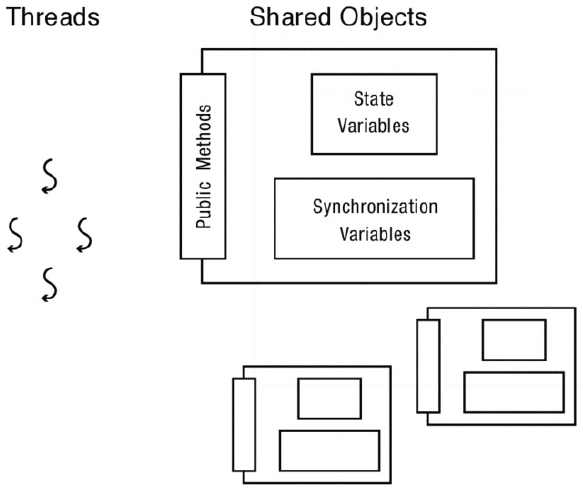
\includegraphics[scale=0.45]{img/fig0501}}
\caption{En un programa multi-hilo, los hilos están separados y operan simultáneamente en objetos compartidos. Los objetos compartidos contienen ambas variables de estado y sincronización compartidas, que se utilizan para controlar el acceso concurrente a estado compartido.}
\label{fig0501}
\end{figure}

Décadas de trabajo han permitido desarrollar un enfoque mucho más simple para escribir programas multihilo que el uso de cargas y almacenamientos atómicos. Este enfoque extiende la modularidad de la programación orientada a objetos a programas multi-hilo. Como ilustra la \textit{Fig.} \ref{fig0501}, un programa multi-hilo se construye a partir de objetos compartidos y un conjunto de hilos que operan en ellos.

Los objetos compartidos son objetos que se pueden acceder de manera segura por varios hilos. Todos estos recursos compartidos en un programa -- incluyendo variables asignadas en el \textit{heap} (por ejemplo, objetos asignados con {\mf malloc} o {\mf new}) y, variables globales estáticas -- debe ser encapsulado en uno o más objetos compartidos.

Programar con objetos compartidos extiende la programación tradicional orientado a objetos, en la cual los objetos ocultan sus detalles de implementación detrás de una interfaz limpia. De la misma manera, los objetos compartidos ocultan los detalles de la sincronización de las acciones de múltiples hilos detrás de una interfaz limpia. Los hilos que utilizan objetos compartidos sólo necesitan entender la interfaz; ellos no necesitan saber cómo el objeto compartido maneja internamente la sincronización.

Al igual que los objetos normales, los programadores pueden diseñar objetos compartidos para cualesquiera módulos, interfaces y semántica que necesite la aplicación. Cada clase de objeto compartido define un conjunto de métodos públicos en los que el hilo opera. Para ensamblar el programa entero a partir de estos objetos compartidos, cada hilo se ejecuta un ``bucle principal'', escrito en términos de acciones sobre los métodos públicos de objetos compartidos.

Dado que los objetos compartidos encapsulan el estado compartido del programa, el código del bucle principal que define medidas de alto nivel de un hilo no necesita preocuparse por los detalles de sincronización. Así, el modelo de programación se ve muy similar a la del código de un solo hilo.

\subsection{La implementación de objetos compartidos}
Por supuesto, a nivel interno los objetos compartidos deben manejar los detalles de sincronización. Los objetos compartidos se aplican en capas.
\begin{itemize}
\item \textbf{Capa de objeto compartido}. Al igual que en la programación orientada a objetos estándar, los objetos compartidos definen la lógica específica de la aplicación y ocultan detalles internos de implementación. Externamente, parecen tener la misma interfaz que se debiese definir para un programa de un solo hilo.

\item \textbf{Capa de variable de sincronización}. En lugar de implementar objetos compartidos directamente intercalando cuidadosamente las cargas y almacenamientos atómicos, los objetos compartidos incluyen \textit{variables de sincronización} como variables miembro. Las variables de sincronización, almacenadas en la memoria al igual que cualquier otro objeto, pueden incluirse en cualquier estructura de datos.

Una \textbf{variable de sincronización} es una estructura de datos utilizada para coordinar el acceso simultáneo a estado compartido. Tanto la interfaz y la implementación de las variables de sincronización deben ser cuidadosamente diseñadas. En particular, podemos construir objetos compartidos utilizando dos tipos de variables de sincronización: \textbf{Cerrojos} (\textit{locks}) y \textbf{Variables de Condición} (\textit{condition variables}).

Las variables de sincronización coordinan el acceso a las variables de estado, que son sólo las variables miembros normales de un objeto de la programación a partir de un único hilo (por ejemplo, enteros, cadenas, arreglos y punteros).

El uso de variables de sincronización simplifica la implementación de objetos compartidos. De hecho, no sólo los objetos compartidos se parecen externamente a objetos de un único hilo tradicionales, pero, mediante la implementación con variables de sincronización, sus implementaciones internas son bastante similares a las de los programas de un solo hilo.

\item \textbf{La capa de instrucción atómica}. A pesar de que las capas superiores se benefician de un modelo de programación más simple, no todo es tan sencillo. Internamente, las variables de sincronización deben gestionar las intercalaciones de acciones de diferentes hilos.

En lugar de implementar las variables de sincronización, tales como cerrojos y variables de condición, utilizando cargas y almacenamientos atómicos, como hemos tratado de hacer en el problema de demasiada leche, las implementaciones modernas construyen las variables de sincronización utilizando instrucciones de \textit{lectura-modificación-escritura atómicas}. Estas instrucciones específicas del procesador permiten a un hilo tener temporalmente acceso de forma exclusiva y atómica a una ubicación de memoria mientras se ejecuta la instrucción. Típicamente, la instrucción atómicamente lee una posición de memoria, hace alguna operación aritmética simple con el valor, y almacena el resultado. El hardware garantiza que las instrucciones de cualquier otro hilo con el acceso a misma posición de memoria se producen ya sea por completo antes de, o en su totalidad después de, la instrucción de lectura-modificación-escritura atómica.
\end{itemize}


\section{Locks (Cerrojos): Exclusión Mutua}
Un \textbf{cerrojo} es una variable de sincronización que proporciona la exclusión mutua -- cuando un hilo mantiene un cerrojo, ningún otro hilo puede mantenerlo (es decir, otros hilos están excluidos). Un programa tiene asociado cada cerrojo con algún subconjunto de estado compartido y requiere un hilo para mantener el cerrojo al acceder a ese estado. Entonces, sólo un hilo puede acceder al estado compartido a la vez.

La exclusión mutua simplifica en gran medida el razonamiento acerca de los programas ya que un hilo puede realizar un conjunto arbitrario de operaciones, mientras que mantiene un cerrojo, y esas operaciones parecen ser atómicas a otros hilos. En particular, debido a que un cerrojo hace cumplir la exclusión mutua y los hilos deben sostener el cerrojo para acceder a estos recursos compartidos, ningún otro hilo puede observar un estado intermedio. Otros procesos únicamente pueden observar el estado dejado luego de la liberación del cerrojo.

\textbf{Cerrojos para agrupar varias operaciones}. Consideremos, por ejemplo, un objeto de cuenta bancaria que incluye una lista de transacciones y un balance total. Para añadir una nueva transacción, se adquiere el cerrojo de la cuenta, se añade la nueva transacción a la lista, se lee el antiguo balance, se lo modifica, se escribe el nuevo balance, y se libera el cerrojo. Para consultar el saldo y la lista de transacciones recientes, se adquiere el cerrojo de la cuenta, se lee la lista de transacciones recientes, se consulta el balance y se libera el cerrojo. El uso de cerrojos de esta manera garantiza que una actualización o una consulta se complete antes de que comience la siguiente. Cada consulta siempre refleja el conjunto completo de transacciones recientes.

Otro ejemplo de agrupación es una salida de impresión. Sin cerrojos, si dos hilos llaman a {\mf printf} al mismo tiempo, los caracteres individuales de los dos mensajes podrían ser intercalados, tergiversando su significado. En cambio, en los sistemas operativos modernos multi-hilo, {\mf printf} utiliza un cerrojo para asegurar que el grupo de caracteres en cada mensaje es impreso como una unidad.

Es mucho más fácil de razonar acerca de intercalación de grupos atómicos de operaciones en lugar de intercalar las operaciones individuales por dos razones. En primer lugar, hay un menor número (obviamente) de intercalaciones a considerar. El razonamiento sobre las intercalaciones sobre una base más gruesa reduce el número de casos a considerar. En segundo lugar, y lo que es más importante, podemos hacer que cada grupo atómico de operaciones se corresponda con la estructura lógica del programa, lo que nos permite razonar sobre invariantes, y no sobre intercalaciones específicas.

En particular, los objetos compartidos por lo general tienen un cerrojo que guarda todos los estados de un objeto. Cada método público adquiere el cerrojo a la entrada y lo libera a la salida. Por lo tanto, el razonamiento sobre el código de una clase compartida es similar a razonar sobre el código de una clase tradicional: se asume un conjunto de invariantes cuando se llama a un método público y se restablecen esas invariantes antes de que el método público retorne. Si definimos así nuestros invariantes, podemos razonar acerca de cada método de forma independiente.

\subsection{Cerrojos: API y Propiedades}
Un cerrojo permite la exclusión mutua, proporcionando dos métodos: {\mf Lock::acquire()} y {\mf Lock::release()}. Estos métodos se definen como sigue:
\begin{itemize}
\item Un cerrojo puede estar en uno de dos estados: OCUPADO o LIBRE.
\item Un cerrojo se encuentra inicialmente en el estado LIBRE.
\item {\mf Lock::acquire()} espera hasta que el cerrojo esté LIBRE y luego atómicamente pasa al bloqueo a OCUPADO. La comprobación del estado para ver si está LIBRE y el establecimiento del estado de OCUPADO están juntos en una operación atómica. Incluso si varios hilos intentan adquirir el cerrojo, a lo sumo un hilo tendrá éxito. Un hilo observa que el cerrojo está LIBRE y lo establece en OCUPADO; los otros hilos acaban de ver que el cerrojo está OCUPADO y esperan.
\item {\mf Lock::release()} pasa el cerrojo a LIBRE. Si hay operaciones pendientes de {\mf Lock::acquire()}, este cambio de estado hace que uno de ellos proceda.
\end{itemize}

El uso de cerrojos hace que la solución del problema \textit{too much milk} sea trivial. Ambos hilos corren el siguiente código:

\begin{lstlisting}
lock.acquire();
if (milk == 0) {		// si no hay leche
	milk++;				// comprar leche
}
lock.release();
\end{lstlisting}

\subsection{Semáforos}
Los \textbf{semáforos} fueron introducidos por Dijkstra en 1965 para proporcionar sincronización dentro del sistema operativo. Entre los avances introducidos en el diseño de sistemas operativos se puede mencionar las formas estructuradas de utilización de la concurrencia.

Lo semáforos se definen como sigue:
\begin{itemize}
\item Un semáforo tiene un valor entero no negativo ($\geq 0$).
\item Cuando un semáforo es creado, su valor puede ser inicializado en cualquier valor entero no negativo.
\item {\mf Semaphore::P()} espera hasta que el valor sea positivo. Luego, decrementa su valor de manera atómica en 1 y retorna.
\item {\mf Semaphore::V()} incrementa de manera atómica el valor en 1. Si hay hilos esperando en {\mf P}, entonces uno de ellos es habilitado, de forma que la llamada a {\mf P} pueda decrementar exitosamente el valor y retornar.
\item No se permiten otras operaciones en un semáforo. En particular, ningún hilo puede leer directamente el valor del semáforo.
\end{itemize}

Las acciones de comprobar el valor y modificarlo se realizan en conjunto como una sola acción atómica indivisible. Se garantiza que, una vez que empieza una operación de semáforo, ningún otro proceso podrá acceder al semáforo sino hasta que la operación se haya completado o bloqueado. Esta atomicidad es absolutamente esencial para resolver problemas de sincronización y evitar condiciones de carrera.

La operación {\mf V()} incrementa el valor del semáforo direccionado. Si uno o más procesos estaban inactivos en ese semáforo, sin poder completar una operación {\mf P()} anterior, el sistema selecciona uno de ellos (al azar) y permite que complete su operación {\mf P()} . Así, después de una operación {\mf V()} en un semáforo que contenga procesos inactivos, el semáforo seguirá en 0 pero habrá un proceso inactivo menos en él. La operación de incrementar el semáforo y despertar a un proceso (sacar de la suspensión) también es indivisible. Ningún proceso se bloquea al realizar una operación {\mf V()}.

Lo normal es implementar {\mf V()} y {\mf P()} como llamadas al sistema, en donde el sistema operativo deshabilita brevemente todas las interrupciones, mientras evalúa el semáforo, lo actualiza y suspende el proceso, si es necesario. Como todas estas acciones requieren sólo unas cuantas instrucciones, no se corre peligro al deshabilitar las interrupciones. Si se utilizan varias CPUs, cada semáforo debe estar protegido por una variable \textit{lock} para asegurar que sólo una CPU a la vez pueda examinar el semáforo.

Los sistemas operativos diferencian a menudo entre semáforos contadores y semáforos binarios. El valor de un \textbf{semáforo contador} puede variar en un dominio no restringido, mientras que el valor del \textbf{semáforo binario} sólo puede ser 0 ó 1. En algunos sistemas, los semáforos binarios se conocen como \textbf{cerrojos mútex}, ya que son cerrojos que proporcionan exclusión mutua. Cuando el recurso está disponible, un proceso accede y decrementa el valor del semáforo con la operación {\mf P()}. El valor queda entonces en 0, lo que hace que si otro proceso intenta decrementarlo tenga que esperar. Cuando el proceso que decrementó el semáforo realiza una operación {\mf V()}, algún proceso que estaba esperando comienza a utilizar el recurso.

Los semáforos contadores se pueden utilizar para controlar el acceso a un determinado recurso formado por un número finito de instancias. El semáforo se inicializa con el número de recursos disponibles. Cada proceso que desee usar un recurso ejecuta una operación {\mf P()} en el semáforo (decrementando la cuenta). Cuando un proceso libera un recurso, ejecuta una operación {\mf V()} (incrementando la cuenta). Cuando la cuenta del semáforo llega a 0, todos los recursos estarán en uso. Después, los procesos que deseen usar un recurso se bloquearán hasta que la cuenta sea mayor a que 0.

También podemos usar los semáforos para resolver diversos problemas de sincronización. Por ejemplo, considere dos procesos que se estén ejecutando de forma concurrente: {\mf P1} con una instrucción {\mf S1} y {\mf P2} con una instrucción {\mf S2}. Suponga que necesitamos que {\mf S2} se ejecute sólo después que {\mf S1} se haya completado. Podemos implementar este esquema dejando que {\mf P1} y {\mf P2} compartan un semáforo común {\mf synch}, inicializado con el valor 0, e insertando las instrucciones:

\begin{lstlisting}
S1;
V(synch);
\end{lstlisting}

en el proceso {\mf P1}, y las instrucciones

\begin{lstlisting}
S2;
P(synch);
\end{lstlisting}

en el proceso {\mf P2}. Dado que {\mf synch} se inicializa con el valor 0, {\mf P2} ejecutará {\mf S2} sólo después de que {\mf P1} haya invocado {\mf V(synch)}, instrucción que sigue a la ejecución de {\mf S1}.

\setcounter{chapter}{6}
\chapter{Scheduling - Planificación}
Cuando hay varias cosas por hacer, ¿cómo podemos elegir qué hacer primero? En los últimos capítulos, hemos descrito cómo crear subprocesos, intercalar entre ellos y sincronizar su acceso a los datos compartidos. En momento dado, algunos subprocesos se están ejecutando en el procesador. Otros están esperando su turno para ocupar el procesador. Mientras otros se bloquean esperando que se complete alguna E/S, se señale una variable de condición o se libere un bloqueo. Cuando hay más subprocesos que procesadores, la \textbf{política de programación del procesador} determina qué subprocesos ejecutar primero.

Podríamos pensar que la respuesta a esta pregunta es fácil: simplemente haga el trabajo en el orden en que llega. Después de todo, eso parece ser la única cosa justa a hacer. Hay una razón por la cual, como veremos más adelante en este capítulo, hacer las cosas por orden de llegada es a veces lo peor que puedes hacer en términos de mejorar el tiempo de respuesta percibido por el usuario.

Se podría pensar que la respuesta a esta pregunta no es importante. Con la mejora de millones de veces en el rendimiento del procesador en los últimos treinta años, podría parecer que somos un millón de veces menos propensos a tener nada esperando su turno de ocupar un procesador. Pero en verdad esto no es así, los sistemas operativos del servidor en particular son a menudo sobrecargados. Las aplicaciones paralelas pueden crear más cantidad de trabajo que procesadores existentes, y si no se toma en cuenta en el diseño de la política de planificación, el rendimiento puede degradarse gravemente. Hay relaciones sutiles entre la política de planificación y la administración de energía en los dispositivos con baterías, como los smartphones y las laptops. Además, los problemas de planificación se aplican a cualquier recurso escaso, ya sea que la fuente de contención sea el procesador, la memoria, el disco o la red.

La política de programación no es una panacea. Sin suficiente capacidad, el rendimiento puede ser pobre, independientemente del hilo que ejecutamos primero.

Afortunadamente, es probable que tengas un poco de intuición en cuanto al impacto de diferentes políticas y capacidad de planificación en temas como tiempo de respuesta, imparcialidad y rendimiento. Cualquier persona que espera en una fila probablemente se pregunta cómo podríamos ir más rápidamente. Eso es cierto si estamos esperando en la fila en el supermercado, un banco, o en un restaurante popular. Sorprendentemente, en cada uno de estos entornos, hay un enfoque diferente de cómo se ocupan de la espera. Intentaremos responder por qué.

No hay una respuesta correcta; Más bien, cualquier política de planificación plantea un conjunto complejo de compensaciones entre varias propiedades deseables. El objetivo de este capítulo no es enumerar todas las posibilidades interesantes, explorar el espacio de diseño completo, ni siquiera identificar políticas útiles específicas. En cambio, describimos algunos de las compensaciones e intentamos ilustrar cómo un diseñador puede abordar el problema de seleccionar una política de planificación.

\textbf{Terminología de Rendimiento:}

\begin{itemize}
\item \textbf{Task - Tarea}. Una solicitud de usuario. Una tarea también se llama a menudo un trabajo. Una tarea puede ser de cualquier tamaño, desde simplemente volver a dibujar la pantalla para mostrar el movimiento del cursor del ratón hasta calcular la forma de una proteína recién descubierta. Cuando hablamos de planificación, usamos el término tarea, en lugar de hilo o proceso, porque un solo hilo o proceso puede ser responsable de múltiples solicitudes o tareas de usuario. Por ejemplo, en un procesador de palabras, cada carácter escrito es una solicitud de usuario individual para agregar ese carácter al archivo y mostrar el resultado en la pantalla.
\item \textbf{Response Time- Tiempo de respuesta (o Retardo)}. El tiempo percibido por el usuario para hacer alguna tarea.
\item \textbf{Predictability - Previsibilidad}. Baja variación en los tiempos de respuesta para solicitudes repetidas.
\item \textbf{Throughput - Rendimiento}. La velocidad a la que se completan las tareas.
\item \textbf{Scheduling Overhead - Sobrecarga de Planificación}. El tiempo para cambiar de una tarea a otra.
\item \textbf{Fairness - Equidad}. Igualdad en el número y puntualidad de los recursos asignados a cada tarea.
\item \textbf{Starvation - Inanición}. La falta de progreso de una tarea, debido a que los recursos fueron asignados a una tarea de mayor prioridad.
\end{itemize}

\section{Planificación de un solo Procesador}
Comenzamos con tres políticas sencillas: \textit{First-In-First-Out}, \textit{Shortest-Job-First} y \textit{Round-Robin} (primero en entrar-primero en salir, primero el mas corto y en ronda), como una forma de ilustrar los conceptos de programación. Cada enfoque tiene sus propias fortalezas y debilidades, y la mayoría de los sistemas de asignación de recursos (ya sea para procesadores, memoria, red o disco) combinan aspectos de los tres. Al final de la discusión, mostraremos cómo los diferentes enfoques se pueden sintetizar en un planificador de procesador más práctico y completo.

Antes de proceder, necesitamos definir algunos términos. Una carga de trabajo (\textit{workload}) es un conjunto de tareas que debe realizar un sistema, junto con el momento en que llega cada tarea y cuánto tarda cada tarea en completarse (cuándo llega y cuánto tarda cada tarea). En otras palabras, la carga de trabajo define la entrada a un algoritmo de planificación. Dada una carga de trabajo, un planificador de procesador decide cuándo se asigna cada tarea al procesador.

Estamos interesados en programar algoritmos que funcionen bien en una amplia variedad de entornos, ya que las cargas de trabajo variarán bastante de sistema a sistema y de usuario a usuario. Algunas tareas se calculan y sólo utilizan el procesador. Otros, como un compilador o un navegador web, mezclan E/S y computo. Otros, como una descarga de BitTorrent, están vinculados a E/S, pasando la mayor parte de su tiempo esperando por E/S y sólo por períodos cortos de computo. En la discusión, comenzamos con cargas de trabajo muy complejas y luego generalizamos para incluir mezclas de diferentes tipos de tareas a medida que avanzamos.

Algunas de las políticas que describimos son la mejor política posible sobre una métrica y una carga de trabajo concretas, y algunas son la peor política posible. Al discutir cuan óptima o pésima es una política, sólo estamos comparando con las políticas que son de conservación del trabajo. Un programador es conservador de trabajo si nunca deja el procesador inactivo si hay trabajo que hacer. Obviamente, una política trivialmente pobre tiene el procesador sentado inactivo durante largos períodos cuando hay tareas en la \textit{Ready List}.

Nuestra discusión asume también que el planificador tiene la capacidad de \textbf{pausar} (\textit{preempt}) al procesador y de darlo a alguna otra tarea. La Preemption puede ocurrir debido a una interrupción del temporizador, o porque alguna tarea llega a la \textit{Ready List} con una prioridad más alta que la tarea actual, al menos de acuerdo con alguna política de programación.

\subsection{Primero en entrar, primero en salir (FIFO)}
Tal vez el algoritmo de programación más simple es \textbf{FIFO}: hacer cada tarea en el orden en que llega. FIFO a veces también se llama primero llegado primero servido, o \textbf{FCFS}. Cuando empezamos a trabajar en una tarea, seguimos funcionando hasta que termina. FIFO minimiza la sobrecarga, cambiando entre las tareas sólo cuando cada una esta completa. Debido a que minimiza la sobrecarga, si tenemos un número fijo de tareas, y esas tareas sólo necesitan el procesador, FIFO tendrá el mejor rendimiento: se completará la mayoría de las tareas más rápidamente. Y como mencionamos, FIFO parece ser la definición de la justicia - cada tarea espera pacientemente su turno.

Desafortunadamente, FIFO tiene una debilidad. Si una tarea corta con muy poco trabajo llega despues de comenzada una tarea que toma un tiempo muy largo, entonces el sistema parecerá muy ineficiente. La Figura \ref{fig0701} ilustra una carga de trabajo particularmente mala para FIFO. Si la primera tarea de la cola toma un segundo, y los cuatro siguientes llegan un instante después, pero cada uno sólo necesita un milisegundo del procesador, entonces todos tendrán que esperar hasta que termine el primero. El tiempo de respuesta promedio será más de un segundo, pero el tiempo de respuesta promedio óptimo es mucho menor que eso. De hecho, si ignoramos la conmutación de gastos generales, hay algunas cargas de trabajo donde FIFO es literalmente la peor política posible para el tiempo de respuesta promedio.

\textbf{FIFO y Memcached}

Aunque usted puede pensar que FIFO es demasiado simple para ser útil, hay algunos casos importantes donde es exactamente la elección correcta para la carga de trabajo. Un ejemplo de ello es memcached. Muchos servicios web, como Facebook, almacenan sus datos de usuario en una base de datos. La base de datos proporciona búsquedas flexibles y coherentes, como por ejemplo, qué amigos deben ser notificados de una actualización concreta en el muro de un usuario.

Con el fin de mejorar el rendimiento, Facebook y otros sistemas ponen un caché llamado memcached frente a la base de datos, de modo que si un usuario envía dos elementos a su muro, el sistema sólo tiene que buscar la lista de amigos una vez. El sistema comprueba primero si la información se almacena en caché y, si es así, utiliza esa copia.

Debido a que casi todas las solicitudes son para pequeñas cantidades de datos, memcached responde a peticiones en orden FIFO. Esto minimiza la sobrecarga, ya que no hay necesidad de intervalo de tiempo entre las solicitudes. Para esta carga de trabajo donde las tareas son aproximadamente iguales en tamaño, FIFO es simple, minimiza el tiempo de respuesta promedio e incluso maximiza el rendimiento. \textit{Win-Win!}

\subsection{El trabajo más corto primero (SJF)}
Si FIFO puede ser una mala elección para el tiempo de respuesta promedio, ¿Existe una política óptima para minimizar el tiempo de respuesta promedio? La respuesta es sí: planificar el trabajo más corto primero (SJF).

Supongamos que podríamos saber cuánto tiempo necesita cada tarea en el procesador. (En general, no lo sabremos, por lo que no se trata de una política práctica, sino que la utilizamos como un experimento de pensamiento, más adelante veremos cómo aproximar a SJF en la práctica). Si siempre planificamos la tarea que tiene el trabajo mas corto por hacer, se minimiza el tiempo de respuesta promedio. (Por esta razón, algunos llaman a SJF shortest-remaining-time-first o \textbf{SRTF}.)

Para ver que el SJF es óptimo, considere una hipotética política alternativa que no sea SJF, pero que creemos que podría ser óptima. Dado que la alternativa no es SJF, en algún momento elegirá ejecutar una tarea que sea más larga que otra en la cola. Si ahora cambiamos el orden de tareas, manteniendo todo igual, pero haciendo la tarea más corta primero, reduciremos el tiempo de respuesta promedio. Por lo tanto, cualquier alternativa a SJF no puede ser óptima.

La Figura \ref{fig0701} ilustra SJF en el mismo ejemplo que usamos para FIFO. Si una tarea larga es la primera en llegar, se programará (si estamos conservando el trabajo). Cuando una tarea corta llega un poco más tarde, el programador prevé la tarea actual, e inicia la más corta. Las restantes tareas cortas serán procesadas en orden de llegada, seguido de terminar la tarea larga.

Lo que cuenta como \textit{más corto} es el tiempo restante en la tarea, no su longitud original. Si estamos a un nanosegundo de terminar una tarea de una hora de duración, minimizaremos el tiempo de respuesta promedio manteniéndonos con esa tarea, en lugar de evitarla por una tarea de un minuto que acaba de llegar a la \textit{Ready List}. Por supuesto, si ambos llegan casi al mismo tiempo, hacer la tarea de un minuto de duración primero mejorará drásticamente el tiempo de respuesta promedio.

¿Tiene SJF otros inconvenientes (aparte de ser imposible de implementar porque requiere conocimiento del futuro)? Resulta que SJF es pesimal para la variación en el tiempo de respuesta. Haciendo las tareas más cortas lo más rápido posible, SJF hace necesariamente tareas más largas lo más lentamente posible (entre las políticas que son conservadoras de trabajo). En otras palabras, existe una compensación fundamental entre reducir el tiempo de respuesta promedio y reducir la varianza en el tiempo de respuesta promedio.

Peor aún, SJF puede sufrir de hambre y frecuentes cambios de contexto. Si llegan suficientes tareas cortas, las tareas largas pueden no completarse. Siempre que una tarea nueva en la \textit{Ready List} sea más corta que el tiempo restante en la tarea actual, el planificador cambiará a la nueva tarea. Si esto sigue sucediendo indefinidamente, una larga tarea puede no terminar nunca.

\begin{figure}[tbhp]
\centerline{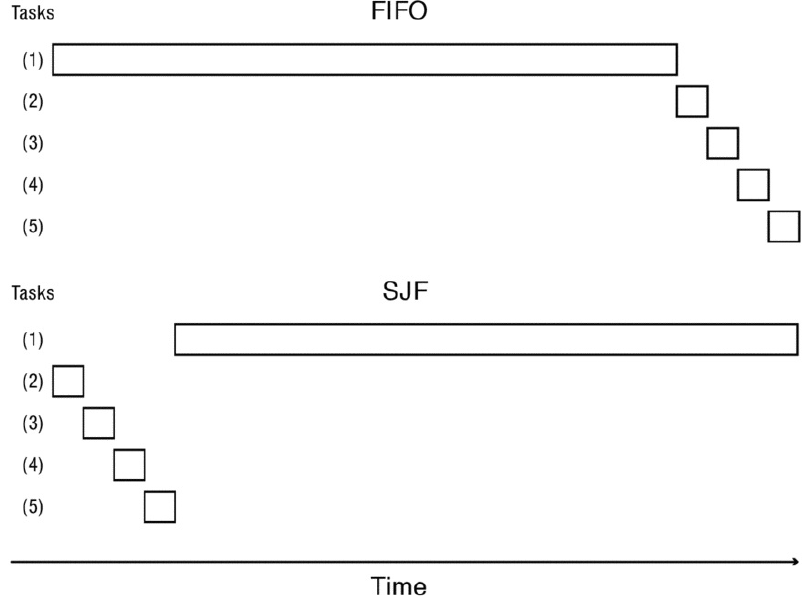
\includegraphics[scale=0.70]{img/fig0701}}
\caption{Los tiempos de finalización con FIFO (arriba) y SJF (abajo) de la planificación cuando varias tareas cortas ($2-5$) llegan inmediatamente después de una tarea larga ($1$).}
\label{fig0701}
\end{figure}

\subsection{Round Robin}
Una política que aborda la inanición es programar las tareas de una manera Round Robin. Con Round Robin, las tareas se turnan ejecutándose en el procesador durante un período limitado de tiempo. El planificador asigna el procesador a la primera tarea en la \textit{Ready List}, estableciendo una interrupción del temporizador para un cierto retardo, llamado el tiempo cuántico. Al final del quantum, si la tarea no se ha completado, la tarea se evita y el procesador se da a la siguiente tarea en la \textit{Ready List}. La tarea anticipada se vuelve a poner en la \textit{Ready List} donde puede esperar su siguiente turno. Con Round Robin, no hay posibilidad de que una tarea sufra de inanición. Finalmente llegará al frente de la cola y obtendrá su tiempo cuántico.


\begin{figure}[tbhp]
\centerline{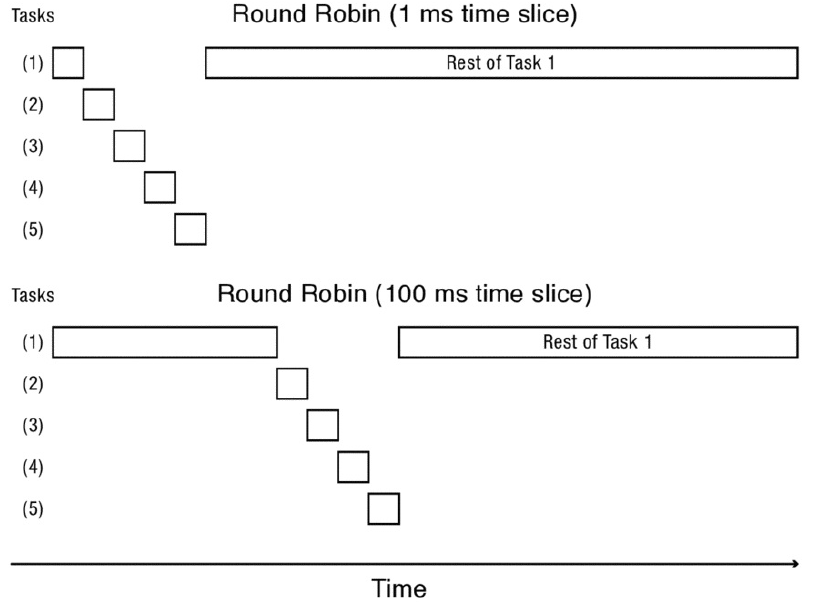
\includegraphics[scale=0.70]{img/fig0702}}
\caption{Tiempos de finalización con la programación Round Robin cuando llegan tareas cortas justo después de una tarea larga, con un tiempo de 1 ms (arriba) y 100 ms (abajo).}
\label{fig0702}
\end{figure}

Por supuesto, tenemos que escoger el quantum de tiempo cuidadosamente. Una consideración es tener en cuenta la sobrecarga: si tenemos un quantum de tiempo demasiado corto, el procesador pasará todo su tiempo cambiando y recibiendo muy poco trabajo útil. Si tomamos un tiempo demasiado largo, las tareas tendrán que esperar mucho tiempo hasta que tengan un turno. La Figura \ref{fig0702} muestra el comportamiento de Round Robin, en la misma carga de trabajo que en la Figura \ref{fig0701}, para dos valores diferentes para el quantum de tiempo.

Una forma de ver Round Robin es como un compromiso entre FIFO y SJF. En un extremo, si el quantum de tiempo es infinito (o al menos, más largo que la tarea más larga), Round Robin se comporta exactamente igual que FIFO. Cada tarea se ejecuta hasta su finalización y luego entrega el procesador a la siguiente en la fila. En el otro extremo, supongamos que fue posible cambiar entre tareas con cero sobrecarga, por lo que podríamos elegir un tiempo cuántico de una sola instrucción. Con el corte de tiempo de grano fino, las tareas terminarían en el orden de longitud, como con SJF, pero más lento: una tarea A se completará dentro de un factor $n$, donde $n$ es el número máximo de tareas ejecutables.

\begin{figure}[tbhp]
\centerline{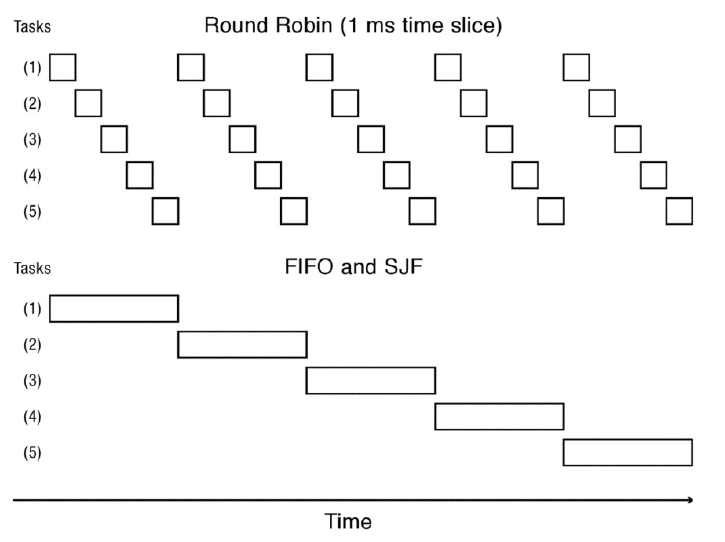
\includegraphics[scale=0.70]{img/fig0703}}
\caption{Tiempos de finalización con Round Robin (arriba) frente a FIFO y SJF (abajo) al programar tareas de igual longitud.}
\label{fig0703}
\end{figure}

Desafortunadamente, Round Robin tiene algunas debilidades. La Figura \ref{fig0703} ilustra lo que sucede para FIFO, SJF y Round Robin cuando varias tareas comienzan aproximadamente a la misma hora y son de la misma longitud. Round Robin girará a través de las tareas, haciendo un poco de cada una, terminando todas en aproximadamente el mismo tiempo. Esta es casi la peor política de programación posible para esta carga de trabajo. FIFO lo hace mucho mejor, escogiendo una tarea y quedándose con ella hasta que termine. No sólo FIFO reduce el tiempo de respuesta promedio para esta carga de trabajo en relación con Round Robin, sino que ninguna tarea es peor con FIFO -cada tarea termina al menos tan pronto como lo haría con Round Robin. Recortar el tiempo de la carga no agrega ningún beneficio. Finalmente, considere lo que SJF hace en esta carga de trabajo. SJF programa tareas en exactamente el mismo orden que FIFO. La primera tarea que llegue se asignará al procesador, y tan pronto como ejecute una sola instrucción, tendrá menos tiempo restante que todas las otras tareas, y por lo tanto se ejecutará hasta su finalización. Dado que sabemos que SJF es óptimo para el tiempo de respuesta promedio, esto significa que tanto FIFO como Round Robin son óptimos para algunas cargas de trabajo y pésimos para otras.

Dependiendo del quantum de tiempo, Round Robin también puede ser bastante pobre cuando se ejecuta una mezcla de tareas vinculadas a E/S y tareas de computo. Las tareas de E/S suelen necesitar períodos muy cortos en el procesador para calcular la operación de E/S siguiente para emitir. Cualquier retraso que se programe en el procesador puede conducir a ralentizaciones en todo el sistema. Por ejemplo, en un editor de texto, a menudo toma sólo unos pocos milisegundos para hacer eco de una pulsación de tecla a la pantalla, un retraso mucho más rápido que la percepción humana. Sin embargo, si estamos compartiendo el procesador entre un editor de texto y varias otras tareas usando Round Robin, el editor debe esperar varios cuantos de tiempo para programar cada golpe de tecla - con un tiempo de $100 ms$, esto puede resultar molesto para el usuario.

\subsection{Max-Min Fairness - Equidad máxima-mínima}
En muchos entornos, una asignación justa de recursos es tan importante para el diseño de un programador como la capacidad de respuesta y la baja sobrecarga. En una máquina multiusuario o en un servidor, no queremos permitir que un solo usuario pueda monopolizar los recursos de la máquina, degradando el servicio para otros usuarios. Aunque puede parecer que la justicia tiene poco valor en las máquinas de un solo usuario, las aplicaciones individuales a menudo son escritas por diferentes compañías, cada una con un interés en hacer que el rendimiento de sus aplicaciones parezca bueno incluso si eso tiene un costo degradante para otras aplicaciones.

Otra complicación surge si debemos asignar recursos de manera justa entre usuarios, aplicaciones, procesos o subprocesos. Algunas aplicaciones pueden ejecutarse dentro de un solo proceso, mientras que otras pueden crear muchos procesos, y cada proceso puede implicar múltiples subprocesos. Round Robin entre los hilos puede conducir a la inanición si las aplicaciones con un solo hilo están compitiendo con las aplicaciones con cientos de hilos. Podemos preocuparnos por la asignación justa en cualquiera de estos niveles de granularidad: hilos dentro de un proceso, procesos para un usuario en particular, usuarios que comparten una máquina física. Por ejemplo, podríamos preocuparnos de asegurarnos de que cada hilo dentro de un proceso progrese. Sin embargo, para simplificar, nuestra discusión supondremos que estamos interesados en proporcionar equidad entre los procesos; los mismos principios se aplican si la unidad que recibe los recursos es el usuario, la aplicación o el hilo.

La equidad es fácil si todos los procesos están calculados: Round Robin dará a cada proceso una parte igual del procesador. En la práctica, sin embargo, diferentes procesos consumen recursos a diferentes ritmos. Un proceso vinculado a E/S puede necesitar sólo una pequeña parte del procesador, mientras que un proceso dependiente de computo está dispuesto a consumir todo el tiempo de procesador disponible. ¿Qué es una asignación equitativa cuando hay una diversidad de necesidades?

Una posible respuesta es decir que cualquier cosa que Round Robin hace es justa, después de todo, cada proceso tiene una oportunidad igual en el procesador. Sin embargo, como vimos anteriormente, Round Robin puede resultar en procesos de E/S que se ejecutan a una velocidad mucho más lenta de lo que lo harían si tuvieran el procesador para sí mismos, mientras que los procesos de computo limitado apenas se ven afectados. ¡Eso no parece justo!

Si bien hay muchas definiciones posibles de equidad, una particularmente útil se llama \textit{Max-Min Fairness}. Max-min imparcialidad iterativamente maximiza la asignación mínima asignada a un proceso particular (usuario, aplicación o hilo) hasta que se asignen todos los recursos. Si todos los procesos están calculados, el comportamiento de max-min es simple: maximizamos el mínimo dando a cada proceso exactamente la misma proporción del procesador, es decir, usando Round Robin.

El comportamiento de la igualdad max-min es más interesante si algunos procesos no pueden usar su parte entera, por ejemplo, porque son de ejecución corta o vinculados a E/S. Si es así, damos a esos procesos toda su solicitud y redistribuimos la parte no utilizada a los procesos restantes. Algunos de los procesos que reciben la porción adicional pueden no ser capaces de usar su totalidad de la parte revisada, por lo que debemos iterar, redistribuyendo cualquier parte no utilizada. Cuando no se satisfacen plenamente las solicitudes restantes, dividimos el resto de manera igual entre todos los procesos restantes.

Una implementación hipotética pero completamente impracticable de max-min sería dar al procesador en cada instante al procedimiento que haya recibido la menor parte del procesador. Sin embargo, ya hemos visto por qué esto no funcionaría bien. Con dos tareas igualmente largas, tan pronto como ejecutamos una instrucción en una tarea, habría recibido más recursos que la otra, por lo que para preservar la \textit{equidad} necesitaríamos cambiar al instante a la siguiente tarea.

Podemos aproximar una asignación de la max-min justo al relajar esta restricción - para permitir que un proceso para adelantarse a su asignación equitativa en un tiempo cuántico. Cada vez que el programador necesita hacer una elección, elige la tarea para el proceso con el menor tiempo acumulado en el procesador. Si un nuevo proceso llega a la cola con mucho menos tiempo acumulado, como la tarea de disco, evitará el proceso, pero de lo contrario el proceso actual completará su quantum. Las tareas pueden llegar hasta una cantidad de tiempo más que su cuota justa, pero a largo plazo la asignación se igualará.

El algoritmo que acabamos de describir fue originalmente definido para la red, y no para el procesador, la planificación. Si compartimos un enlace entre una solicitud de navegador y una descarga larga, obtendremos una respuesta razonable para el navegador si tenemos una asignación justamente justa: el navegador necesita pocos paquetes de red y, por lo tanto, en max-min sus paquetes siempre se programarán antes de Los paquetes de la descarga.

Incluso esta aproximación, sin embargo, puede ser computacionalmente costosa, ya que requiere que las tareas se mantengan en una cola de prioridad. Para algunos entornos de servidor, puede haber decenas o incluso cientos de miles de decisiones de programación que deben hacerse cada segundo. Para reducir la sobrecarga computacional del planificador, la mayoría de los sistemas operativos comerciales utilizan un algoritmo algo diferente, con el mismo objetivo, que describiremos a continuación.

\subsection{Caso de Estudio: Multi-Level Feedback (Retroalimentación Multinivel)}
La mayoría de los sistemas operativos comerciales, incluyendo Windows, MacOS y Linux, usan un algoritmo de programación llamado cola de comentarios de nivel múltiple (MFQ). MFQ está diseñado para lograr varios objetivos simultáneos:
\begin{itemize}
\item \textbf{Sensibilidad}. Ejecutar tareas cortas rápidamente, como en SJF.
\item \textbf{Gastos indirectos bajos}. Minimizar el número de preemptions, como en FIFO, y minimizar el tiempo dedicado a tomar decisiones de planificación.
\item \textbf{Inanición-Libertad}. Todas las tareas deben progresar, como en Round Robin.
\item \textbf{Tarea en segundo plano}. Aplazar las tareas de mantenimiento del sistema, como la desfragmentación del disco, para que no interfieran con el trabajo del usuario.
\item \textbf{Justicia}. Asignar los mínimos recursos posibles del procesador.
\end{itemize}

Al igual que con cualquier sistema real que debe equilibrar varios objetivos contradictorios, el MFQ no logra perfectamente ninguno de estos objetivos. Más bien, se pretende que sea un compromiso razonable en la mayoría de los casos del mundo real. MFQ es una extensión de Round Robin. En lugar de una sola cola, MFQ tiene varias colas Round Robin, cada una con un nivel de prioridad y un quantum de tiempo diferentes. Las tareas con un nivel de prioridad más alto prevén las tareas de menor prioridad, mientras que las tareas del mismo nivel están programadas en la forma de Round Robin. Además, los niveles de prioridad más altos tienen cuantos de tiempo más cortos que los niveles inferiores.

Las tareas se mueven entre los niveles de prioridad para favorecer las tareas cortas sobre las largas. Si una nueva tarea entra en el nivel de prioridad superior. Cada vez que la tarea usa su quantum de tiempo, baja un nivel; Cada vez que la tarea cede al procesador porque está esperando en la E/S, permanece en el mismo nivel (o se eleva un nivel); Y si la tarea se completa, sale del sistema.

Una nueva tarea de cálculo se iniciará como alta prioridad, pero rápidamente se agotará su cantidad de tiempo y cae a la próxima prioridad más baja, y luego a la siguiente. Por lo tanto, una tarea de E/S que necesite sólo una cantidad modesta de computo casi siempre se programará rápidamente, manteniendo el disco ocupado. Las tareas relacionadas con el cálculo se ejecutan con una cantidad de tiempo prolongada para minimizar la sobrecarga de conmutación mientras se comparte el procesador.

Hasta ahora, el algoritmo que hemos descrito no alcanza la libertad de inanición ni la imparcialidad max-min. Si hay demasiadas tareas vinculadas a E/S, las tareas dependientes de computación pueden no recibir tiempo en el procesador. Para combatir esto, el planificador de MFQ monitorea cada proceso para asegurar que está recibiendo su parte justa de los recursos. En cada nivel, Linux realmente mantiene dos colas - tareas cuyos procesos ya han alcanzado su parte justa sólo están programadas si todos los demás procesos a ese nivel también han recibido su parte justa. Periódicamente, cualquier proceso que reciba menos que su cuota justa tendrá sus tareas aumentadas en prioridad; Igualmente, las tareas que reciben más que su parte justa se pueden reducir en prioridad.

El ajuste de la prioridad también aborda el comportamiento estratégico. Desde un punto de vista puramente egoísta, una tarea puede intentar mantener su prioridad alta haciendo una petición de E/S corta inmediatamente antes de que expire su tiempo cuántico. Eventualmente, el sistema detectará esto y reducirá su prioridad a su nivel de participación justa.

\subsection{Resumen}
\begin{itemize}
\item FIFO es simple y minimiza la sobrecarga.
\item Si las tareas son variables en tamaño, el FIFO puede tener un tiempo de respuesta promedio muy bajo.
\item Si las tareas son iguales en tamaño, FIFO es óptima en términos de tiempo de respuesta promedio.
\item Teniendo en cuenta sólo el procesador, SJF es óptimo en términos de tiempo de respuesta promedio.
\item SJF es pésimo en términos de variación en el tiempo de respuesta.
\item Si las tareas son de tamaño variable, Round Robin aproxima a SJF.
\item Si las tareas son iguales en tamaño, Round Robin tendrá un tiempo de respuesta promedio muy bajo.
\item Las tareas que mezclan el procesador y las E/S se benefician de SJF y perjudican bajo Round Robin.
\item La imparcialidad de Max-min puede mejorar el tiempo de respuesta para las tareas de E/S.
\item Round Robin y Max-min evitan la inanición.
\item Mediante la manipulación de la asignación de tareas a las colas de prioridad, un planificador MFQ puede lograr un equilibrio entre la capacidad de respuesta, la baja sobrecarga y la imparcialidad.
\end{itemize}

\chapter{Traducción de Direcciones}
Un número sorprendente de características avanzadas del sistema se habilitan poniendo el sistema operativo en control de la traducción de direcciones, la conversión de la dirección de memoria a la que el programa piensa que hace referencia (la ubicación física de esa celda de memoria). Desde el punto de vista del programador, la traducción de direcciones se realiza de forma transparente - el programa se comporta correctamente a pesar de que su memoria se almacena en algún lugar completamente diferente de donde piensa que se almacena.

Probablemente hayamos aprendido en alguna clase de programación que una dirección de memoria es sólo una dirección. Un puntero en una lista vinculada que contiene la dirección de memoria real de lo que está apuntando. Una instrucción de salto contiene la dirección de memoria real de la siguiente instrucción a ejecutar. ¡Esto es una ficción útil! Para el programador es a menudo mejor no pensar en cómo cada referencia de memoria se convierte en los datos o la instrucción que se hace referencia. En la práctica, hay bastante actividad sucediendo por detrás.

La Traducción de Direcciones es un concepto simple, pero resulta increíblemente poderoso. ¿Qué puede hacer un sistema operativo con la traducción de direcciones? Vamos a listar unos ejemplos:
\begin{itemize}
\item \textbf{Aislamiento del proceso}. La protección del kernel y otras aplicaciones contra código malicioso requiere la capacidad de limitar las referencias de memoria por las aplicaciones. Del mismo modo, la traducción de direcciones puede ser utilizada por las aplicaciones para construir entornos seguros de ejecución segura para extensiones de terceros.

\item \textbf{Comunicación de interproceso}. A menudo, los procesos necesitan coordinarse entre sí, y una manera eficiente de hacerlo es tener los procesos compartidos en una región de memoria común.

\item \textbf{Segmentos de código compartidos}. Las instancias del mismo programa pueden compartir las instrucciones del programa, reduciendo su huella de memoria y haciendo que la caché del procesador sea más eficiente. Del mismo modo, diferentes programas pueden compartir bibliotecas comunes.
\end{itemize}

En este capítulo, nos centraremos en los mecanismos necesarios para implementar la traducción de direcciones, ya que es la base de todos estos servicios. Para la eficiencia en tiempo de ejecución, la mayoría de los sistemas tienen hardware especializado para hacer traducción de direcciones; Este hardware es administrado por el kernel. Sin embargo, en algunos sistemas, la traducción es proporcionada por un compilador, un vinculador o un intérprete de código de bytes de confianza. En otros sistemas, la aplicación realiza la traducción del puntero como una forma de administrar el estado de sus propias estructuras de datos. En otros sistemas todavía, se utiliza un modelo híbrido donde las direcciones se traducen tanto en software como en hardware. La elección suele ser un compromiso de ingeniería entre rendimiento, flexibilidad y costo. Sin embargo, la funcionalidad proporcionada es a menudo la misma independientemente del mecanismo utilizado para implementar la traducción. En este capítulo, cubriremos una gama de mecanismos de hardware y software.

\section{Concepto de Traducción de Direcciones}
\begin{figure}[tbhp]
\centerline{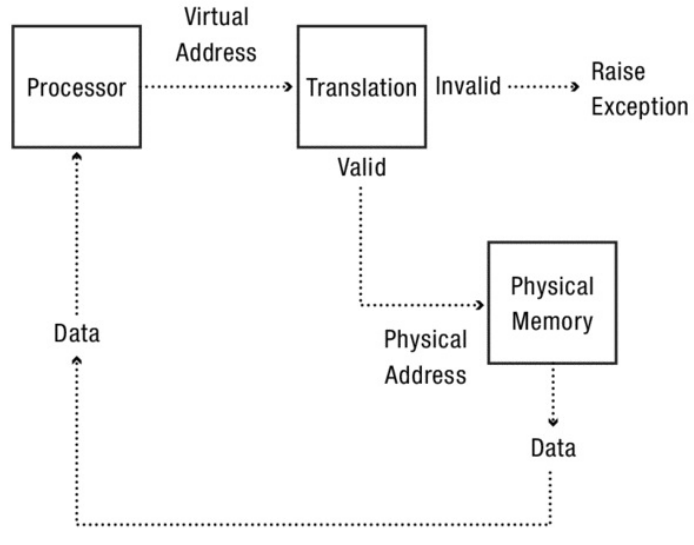
\includegraphics[scale=0.70]{img/fig0801}}
\caption{El traductor convierte direcciones de memoria (virtuales) generadas por el programa en direcciones de memoria física.}
\label{fig0801}
\end{figure}

Considerada como una caja negra, la traducción de direcciones es una función simple, ilustrada en la Figura \ref{fig0801}. El traductor toma cada instrucción y referencia de memoria de datos generada por un proceso, comprueba si la dirección es legal y la convierte en una dirección de memoria física que puede usarse para buscar o almacenar instrucciones o datos. Los datos en sí (lo que se almacena en la memoria) se devuelve tal cual; no se transforma de ninguna manera. La traducción se implementa generalmente en hardware, y el kernel configura el hardware para lograr sus objetivos.

La tarea de este capítulo es mostrar los detalles sobre cómo funciona esa caja negra. Si le preguntamos ahora cómo podría implementarlo, sus primeras varias conjeturas probablemente estarían en lo cierto. Si dijiste que podríamos usar una matriz, un árbol o una tabla hash, tendrías razón: todos estos enfoques han sido tomados por sistemas reales.

Dado que son posibles varias implementaciones diferentes, ¿Cómo evaluar las alternativas? Estas son algunas de las metas que podríamos desear de una caja de traducción; El diseño con el que acabamos dependerá de cómo equilibremos entre estos diversos objetivos.

\begin{itemize}
\item \textbf{Protección de la memoria}. Necesitamos la capacidad de limitar el acceso de un proceso a ciertas regiones de memoria, por ejemplo, para evitar que acceda a la memoria que no pertenece al proceso. A menudo, sin embargo, puede que quiera limitar el acceso de un programa a su propia memoria, por ejemplo, para evitar que un error de puntero sobrescriba la región de código o provocar una \textit{trap} al depurador cuando el programa hace referencia a una ubicación de datos específica.

\item \textbf{Compartir memoria}. Queremos permitir que varios procesos compartan regiones de memoria seleccionadas. Estas regiones compartidas pueden ser grandes (por ejemplo, si compartimos el segmento de código de un programa entre varios procesos que ejecutan el mismo programa) o relativamente pequeñas (por ejemplo, si compartimos una biblioteca común, un archivo o una estructura de datos compartida).

\item \textbf{Ubicación flexible de la memoria}. Queremos permitir al sistema operativo la flexibilidad de colocar un proceso (y cada parte de un proceso) en cualquier parte de la memoria física; Esto nos permitirá empaquetar la memoria física de manera más eficiente. Como veremos en el próximo capítulo, la flexibilidad en la asignación de datos de proceso a ubicaciones de memoria física también nos permitirá hacer un uso más efectivo de cachés en el chip.

\item \textbf{Direcciones dispersas}. Muchos programas tienen varias regiones de memoria dinámica que pueden cambiar de tamaño en el curso de la ejecución del programa: el montículo de objetos de datos, una pila para cada subproceso y archivos mapeados de memoria. Los procesadores modernos tienen espacios de direcciones de $64$ bits, lo que permite a cada objeto dinámico espacio suficiente para crecer según sea necesario, pero la traducción más compleja.

\item \textbf{La eficiencia de búsqueda en tiempo de ejecución}. La traducción de direcciones de hardware se produce en cada búsqueda de instrucciones y en cada carga y almacenamiento de datos. Sería impráctico que una búsqueda tuviera, en promedio, mucho más tiempo de ejecución que la instrucción misma. Al principio, muchos de los esquemas que discutimos parecerán descabelladamente imprácticos! Discutiremos maneras de hacer eficientes los sistemas de traducción más complicados.

\item \textbf{Tablas de traducción compacta}. También queremos que la sobrecarga de espacio de la traducción sea mínima; Cualquier estructura de datos que necesitamos debe ser pequeña en comparación con la cantidad de memoria física que se está administrando.

\item \textbf{Portabilidad}. Las diferentes arquitecturas de hardware hacen diferentes opciones en cuanto a cómo implementan la traducción; Si un kernel del sistema operativo debe ser fácilmente portátil a través de múltiples arquitecturas de procesador, necesita ser capaz de mapear desde sus estructuras de datos (independientes del hardware) a las capacidades específicas de cada arquitectura.
\end{itemize}

Terminaremos con un mecanismo de traducción de direcciones bastante complejo, por lo que nuestra discusión comenzará con los mecanismos más sencillos posibles y agregará funcionalidad solo según sea necesario. Durante la discusión será útil tener en cuenta las dos visiones de la memoria: el proceso ve su propia memoria, usando sus propias direcciones. Llamaremos a estas \textbf{direcciones virtuales}, porque no necesariamente corresponden a ninguna realidad física. Por el contrario, para el sistema de memoria, sólo hay \textbf{direcciones físicas} (ubicaciones reales en la memoria). Desde la perspectiva del sistema de memoria, se le dan direcciones físicas y realiza búsquedas y almacena valores. El mecanismo de traducción convierte entre las dos vistas: \textit{de una dirección virtual a una dirección de memoria física}.

\section{Hacia una traducción flexible de direcciones}
Nuestra discusión de la traducción de direcciones de hardware se divide en dos pasos. En primer lugar, ponemos a un lado la cuestión de la eficiencia de búsqueda y consideramos la mejor manera de lograr los otros objetivos enumerados anteriormente: asignación de memoria flexible, eficiencia espacial, protección y compartición de grano fino, etc. Una vez que tengamos las características que queremos, entonces agregamos mecanismos para ganar la eficiencia de búsqueda posterior.

Hemos ilustrado la noción de protección de la memoria del hardware utilizando el hardware más simple imaginable: \textit{base y límite}. La caja de traducción consta de dos registros adicionales por proceso. El \textbf{registro base} especifica el inicio de la región de memoria física del proceso; El \textbf{registro límite} especifica el alcance de esa región. Si el registro base se agrega a cada dirección generada por el programa, entonces ya no necesitamos un cargador de reubicación (las direcciones virtuales del programa comienzan desde $0$ y van hasta el límite), y las direcciones físicas comienzan desde la base y van hasta la base $+$ límite. Dado que la memoria física puede contener varios procesos, el núcleo restablece el contenido de los registros de base y de límites en cada cambio de contexto de proceso a los valores apropiados para ese proceso.

La traducción de base y límite es simple y rápida, pero carece de muchas de las características necesarias para apoyar programas modernos. La traducción de base y límite sólo soporta la protección de grano grueso a nivel de todo el proceso; No es posible evitar que un programa sobrescriba su propio código, por ejemplo. También es difícil compartir regiones de memoria entre dos procesos. Puesto que la memoria para un proceso necesita ser contigua, soportar regiones de memoria dinámica, tal como para pilas, pilas de hilos o archivos mapeados en memoria, resulta difícil e imposible.

\subsection{Segmentación de Memoria}
Muchas de las limitaciones de la traducción de base y límite se pueden remediar con un pequeño cambio: en lugar de mantener sólo un par de registros de base y de límite por proceso, el hardware puede soportar una matriz de pares de registros de base y de límite para cada proceso. Esto se llama \textbf{segmentación}. Cada entrada en la matriz controla una porción o segmento del espacio de direcciones virtual. La memoria física para cada segmento se almacena de forma contigua, pero se pueden almacenar diferentes segmentos en diferentes ubicaciones. Los bits de orden superior de la dirección virtual se utilizan para indexar en la matriz; El resto de la dirección se trata entonces como se ha añadido anteriormente a la base y se comprueba contra el límite almacenado en ese índice. Además, el sistema operativo puede asignar a diferentes segmentos permisos diferentes, por ejemplo, para permitir el acceso de sólo ejecución al código y acceso de lectura y escritura a los datos. En general el número de segmentos se determina por el número de bits para el número de segmento que se reservan en la dirección virtual.

Parece extraño que la memoria segmentada tenga lagunas; La memoria del programa ya no es una sola región contigua, sino que es un conjunto de regiones. Cada segmento diferente comienza en un nuevo límite de segmento. Por ejemplo, el código y los datos no están inmediatamente adyacentes entre sí en el espacio de direcciones virtual o físico.

¿Qué sucede si un programa se ramifica o trata de cargar datos de una de estas brechas? El hardware generará una excepción, atrapada en el kernel del sistema operativo. En los sistemas UNIX, esto todavía se llama un error de segmentación, es decir, una referencia fuera de un segmento legal de la memoria. ¿Cómo un programa evita deambular en una de estas brechas? Los programas correctos no generarán referencias fuera de la memoria válida. Dicho de otra manera, tratar de ejecutar código o leer datos que no existen es probablemente una indicación de que el programa tiene un error en él.

Aunque es fácil de implementar y administrar, la memoria segmentada es notablemente potente y ampliamente utilizada. Por ejemplo, la arquitectura $x86$ está segmentada. Con los segmentos, el sistema operativo puede permitir que los procesos compartan algunas regiones de la memoria mientras se mantienen protegidas otras regiones. Por ejemplo, dos procesos pueden compartir un segmento de código estableciendo una entrada en sus tablas de segmentos para apuntar a la misma región de memoria física, para usar la misma base y los mismos límites. Los procesos pueden compartir el mismo código mientras se trabaja con datos diferentes, configurando la tabla de segmentos para apuntar a diferentes regiones de la memoria física para el segmento de datos.

Del mismo modo, las rutinas de la biblioteca compartida, como una biblioteca de gráficos, pueden colocarse en un segmento y compartirlo entre procesos. Como antes, los datos de la biblioteca estarían en un segmento separado, no compartido. Esto se hace con frecuencia en sistemas operativos modernos con bibliotecas enlazadas dinámicamente. Un problema práctico es que diferentes procesos pueden cargar diferentes números de bibliotecas, por lo que pueden asignar a la misma biblioteca un número de segmento diferente. Dependiendo de la arquitectura del procesador, el uso compartido puede seguir funcionando si el código de la biblioteca utiliza direcciones segmentos-locales, direcciones que son relativas al segmento actual.

También podemos usar segmentos para la comunicación entre procesos, si los procesos reciben permiso de lectura y escritura para el mismo segmento. Los sistemas más modernos tienden a usar segmentos sólo para regiones de memoria de grano más grueso, tales como el código y los datos de toda una biblioteca compartida, en lugar de para cada una de las estructuras de datos dentro de la biblioteca.

Como ejemplo final de la potencia de los segmentos, permiten la gestión eficiente de la memoria asignada dinámicamente. Cuando un sistema operativo reutiliza la memoria o el espacio en disco que se había utilizado anteriormente, primero debe anular el contenido de la memoria o del disco. De lo contrario, los datos privados de una aplicación podrían, inadvertidamente, filtrarse a otra aplicación potencialmente malintencionada. Por ejemplo, puede introducir una contraseña en un sitio web, por ejemplo, para un banco y, a continuación, salir del explorador. Sin embargo, si la memoria física subyacente utilizada por el explorador se vuelve a asignar a un nuevo proceso, la contraseña se podría filtrar a un sitio web malicioso.

El principal inconveniente de la segmentación es la sobrecarga de gestión de un gran número de segmentos de memoria de tamaño variable y de crecimiento dinámico. Con el tiempo, a medida que se crean y terminan los procesos, la memoria física se dividirá en regiones que están en uso y regiones que no están disponibles, es decir, disponibles para asignarse a un nuevo proceso. Estas regiones libres serán de diferentes tamaños. Cuando creemos un nuevo segmento, tendremos que encontrar un lugar libre para él. ¿Deberíamos ponerlo en la región más pequeña abierta donde encajará? ¿La región abierta más grande?

Sin embargo, elegimos colocar nuevos segmentos, a medida que se asigna más memoria, el sistema operativo puede llegar a un punto donde hay suficiente espacio libre para un nuevo segmento, pero el espacio libre no es contiguo. Esto se llama \textbf{fragmentación externa}. El sistema operativo es libre de compactar la memoria para crear espacio sin afectar a las aplicaciones, ya que las direcciones virtuales no cambian cuando reubicamos un segmento en la memoria física. Aún así, la compactación puede ser costosa en términos de sobrecarga del procesador: una configuración típica de servidor tardaría aproximadamente un segundo en compactar su memoria.

Todo esto se vuelve aún más complejo cuando los segmentos de memoria pueden crecer. ¿Cuánta memoria debemos dejar de lado para el heap de un programa? Si ponemos el segmento de heap en una parte de la memoria física con mucho espacio, entonces habremos perdido la memoria si ese programa resulta necesitar sólo un pequeño espacio. Si hacemos lo contrario - poner el segmento de heap en un pequeño trozo de memoria física - entonces tendremos que copiar en otro lugar si cambia de tamaño.

\subsection{Paginación de Memoria}
Una alternativa a la memoria segmentada es la memoria paginada. Con la paginación, la memoria se asigna en trozos de tamaño fijo llamados \textbf{marcos de página}. La traducción de direcciones es similar a cómo funciona con la segmentación. En lugar de una tabla de segmentos cuyas entradas contienen punteros a segmentos de tamaño variable, hay una tabla de páginas para cada proceso cuyas entradas contienen punteros a marcos de página. Debido a que los cuadros de página son de tamaño fijo y tienen una potencia de dos, las entradas de la tabla de páginas solo necesitan proporcionar los bits superiores de la dirección del marco de página, por lo que son más compactos. No hay necesidad de un límite en el offset; Toda la página en la memoria física se asigna como una unidad. 

Lo que parecerá extraño, y tal vez bueno, acerca de la paginación es que mientras un programa piensa en su memoria como lineal, de hecho su memoria puede ser, y normalmente está, esparcida por toda la memoria física en una especie de mosaico abstracto. El procesador ejecutará una instrucción tras otra utilizando direcciones virtuales; Sus direcciones virtuales son todavía lineales. Sin embargo, la instrucción situada al final de una página se ubicará en una región de memoria física completamente diferente de la siguiente instrucción al principio de la página siguiente. Las estructuras de datos parecerán contiguas usando direcciones virtuales, pero una matriz grande puede estar dispersa a través de muchos marcos de páginas físicas.

La paginación aborda la principal limitación de la segmentación: la asignación de espacios libres es muy sencilla. El sistema operativo puede representar la memoria física como un mapa de bits, con cada bit representando un marco de página físico que está libre o en uso. Encontrar un marco libre es sólo una cuestión de encontrar un bit vacío.

También es conveniente compartir la memoria entre procesos: necesitamos configurar la entrada de la tabla de páginas para cada proceso compartiendo una página para que apunte al mismo marco de página física. Para una región compartida grande que abarca varios marcos de página, como una biblioteca compartida, esto puede requerir la configuración de varias entradas de tabla de páginas. Dado que necesitamos saber cuándo liberar la memoria cuando finaliza un proceso, la memoria compartida requiere una contabilidad adicional para realizar un seguimiento de si la página compartida todavía está en uso. La estructura de datos para esto se llama mapa central; Registra información acerca de cada marco de página físico, como las entradas de la tabla de páginas que apuntan a ella.

Muchas de las optimizaciones que hemos discutido en la segmentación también se puede hacer con paginación. Para copy-on-write, necesitamos copiar las entradas de la tabla de páginas y configurarlas como de sólo lectura; al archivar una de estas páginas, podemos hacer una copia real del marco de la página subyacente antes de reanudar el proceso. Del mismo modo, para \textit{cero} en referencia, podemos configurar la entrada de la tabla de páginas en la parte superior de la pila para que sea inválida, causando una trap en el kernel. Esto nos permite extender la pila solamente según sea necesario.

Las tablas de páginas permiten añadir otras características. Por ejemplo, podemos iniciar un programa que se ejecuta antes de que todo su código y datos se carguen en la memoria. Inicialmente, el sistema operativo marca todas las entradas de la tabla de páginas para un nuevo proceso como no válido; Como las páginas se introducen desde el disco, que las marca como páginas de sólo lectura (para páginas de códigos) o de lectura y escritura (para páginas de datos). Sin embargo, una vez que las primeras páginas están en la memoria, el sistema operativo puede iniciar la ejecución del programa en modo de usuario, mientras que el núcleo sigue transfiriendo el resto del código del programa en segundo plano. A medida que el programa se inicia, si sucede saltar a una ubicación que aún no se ha cargado, el hardware provocará una excepción y el núcleo puede bloquear el programa hasta que esa página esté disponible. Además, el compilador puede reorganizar el ejecutable del programa para un inicio más eficiente, uniendo las páginas de inicialización en unas pocas páginas al inicio del programa, superponiendo así la inicialización y cargando el programa desde el disco.

Un inconveniente de la paginación es que mientras que la gestión de la memoria física se vuelve más simple, la gestión del espacio de direcciones virtuales se vuelve más difícil. Los compiladores normalmente esperan que la pila de ejecución sea contigua (en direcciones virtuales) y de tamaño arbitrario; Cada nueva llamada de procedimiento supone que la memoria para la pila está disponible. Del mismo modo, la biblioteca de tiempo de ejecución para asignación de memoria dinámica normalmente espera un montón contiguo. En un proceso de un solo hilo, podemos colocar la pila y el heap en extremos opuestos del espacio de direcciones virtuales, y hacer que crezcan unos hacia otros. Sin embargo, con múltiples subprocesos por proceso, necesitamos múltiples pilas de subprocesos, cada una con espacio para crecer.

Esto se convierte aún más en un problema con espacios de direcciones virtuales de $64$ bits. El tamaño de la tabla de páginas es proporcional al tamaño del espacio de direcciones virtuales, no al tamaño de la memoria física. Cuanto más escaso sea el espacio de direcciones virtuales, más gastos generales se necesitan para la tabla de páginas. La mayoría de las entradas no son válidas, representando partes del espacio de direcciones virtuales que no se utilizan, pero todavía se necesita memoria física para todas las entradas de la tabla de páginas.

Podemos reducir el espacio ocupado por la tabla de páginas eligiendo un marco de página más grande. ¿Qué tamaño debe tener un marco de página? Un marco de página más grande puede perder espacio si un proceso no usa toda la memoria dentro del marco. Esto se llama \textbf{fragmentación interna}. Los trozos de tamaño fijo son más fáciles de asignar, pero pierden espacio si no se utiliza todo el trozo. Desafortunadamente, esto significa que con la paginación, cualquiera de las páginas es muy grande (pérdida de espacio debido a la fragmentación interna), o la tabla de páginas es muy grande (pérdida de espacio) o ambas cosas. Por ejemplo, con páginas de $16$ KB y un espacio de direcciones virtuales de $64$ bits, podríamos necesitar $250$ entradas de tabla de páginas.

\subsection{Traducción de varios niveles}
Si usted fuera a diseñar un sistema eficiente para hacer una búsqueda en un espacio de teclado, probablemente no elegiría una matriz simple. Un árbol o una \textbf{tabla hash} son más apropiados, y de hecho, los sistemas modernos usan ambos. Nos centramos en esta subsección sobre los árboles; Discutiremos tablas hash después.

Muchos sistemas utilizan la traducción de direcciones basada en árboles, aunque los detalles varían de un sistema a otro y la terminología puede ser un poco confusa. A pesar de las diferencias, los sistemas que estamos a punto de describir tienen propiedades similares. Soportan la protección de memoria gruesa y granulada y el uso compartido de la memoria, la colocación flexible de la memoria, la asignación eficiente de la memoria, y la búsqueda eficiente para los espacios de dirección dispersos, incluso para las máquinas $64$ bit.

Casi todos los sistemas de traducción de direcciones de varios niveles usan la paginación como el nivel más bajo del árbol. Las principales diferencias entre los sistemas se encuentran en la forma en que alcanzan la tabla de páginas en la hoja del árbol (ya sea utilizando segmentación más paginación), o múltiples niveles de paginación, o segmentos más múltiples niveles de paginación. 

Hay varias razones para esto:
\begin{itemize}
\item \textbf{Asignación eficiente de memoria}. Al asignar memoria física en marcos de páginas de tamaño fijo, la gestión del espacio libre puede utilizar un mapa de bits simple.

\item \textbf{Transferencias eficientes de disco}. Los discos de hardware se dividen en regiones de tamaño fijo llamadas sectores; Los sectores de disco deben ser leídos o escritos en su totalidad. Al convertir el tamaño de página en un múltiplo del sector del disco, simplificamos las transferencias desde y hacia la memoria, para cargar programas en la memoria, leer y escribir archivos y usar el disco para simular una memoria mayor que la que está físicamente presente en la máquina.

\item \textbf{Búsqueda eficiente}. Describiremos en la siguiente sección cómo podemos usar un caché llamado buffer de traducción para hacer búsquedas rápidas en el caso común; El búfer de traducción almacena las búsquedas en una página. La paginación también permite que las tablas de búsqueda sean más compactas, especialmente importantes en el nivel más bajo del árbol.

\item \textbf{Búsqueda inversa eficiente}. El uso de marcos de página de tamaño fijo también facilita la implementación del mapa central, para pasar de un marco de página físico al conjunto de direcciones virtuales que comparten el mismo marco. Esto será crucial para implementar la ilusión de una memoria virtual infinita en el próximo capítulo.

\item \textbf{Protección y compartición de granularidad de páginas}. Por lo general, cada entrada de tabla en cada nivel del árbol tendrá sus propios permisos de acceso, permitiendo compartir de grano grueso y de grano fino, hasta el nivel del marco de página individual.
\end{itemize}

\textbf{Segmentación Paginada}

Comencemos un sistema con sólo dos niveles de un árbol. Con segmentación paginada, la memoria está segmentada, pero en lugar de que cada entrada de tabla de segmentos apunte directamente a una región contigua de memoria física, cada entrada de tabla de segmentos apunta a una tabla de páginas que a su vez apunta a la memoria que respalda ese segmento. La entrada de tabla de segmentos \textit{bound} describe la longitud de la tabla de páginas, es decir, la longitud del segmento en páginas. Debido a que la paginación se utiliza en el nivel más bajo, todas las longitudes de segmento son un múltiplo del tamaño de página.

Aunque las tablas de segmentos a veces se almacenan en registros de hardware especiales, las tablas de página para cada segmento son bastante más grandes en agregado, por lo que normalmente se almacenan en la memoria física. Para mantener el asignador de memoria simple, el tamaño máximo del segmento se elige generalmente para permitir que la tabla de páginas para cada segmento sea un pequeño múltiplo del tamaño de la página.

Por ejemplo, con direcciones virtuales de $32$ bits y páginas de $4$ KB, podríamos dejar de lado los $10$ bits superiores para el número de segmento, los $10$ bits siguientes para el número de página y $12$ bits para el desplazamiento de página. En este caso, si cada entrada de tabla de página es de $4$ bytes, la tabla de páginas para cada segmento encajaría exactamente en un marco de página física.

\textbf{Paginación Multi-Nivel}

Un enfoque casi equivalente a la segmentación paginada es utilizar múltiples niveles de tablas de páginas. En el procesador Sun Microsystems SPARC, por ejemplo, hay tres niveles de tabla de páginas. La tabla de páginas de nivel superior contiene entradas, cada una de las cuales apunta a una tabla de página de segundo nivel cuyas entradas son punteros a tablas de páginas. En el SPARC, como ocurre con la mayoría de los otros sistemas que utilizan múltiples niveles de tablas de páginas, cada nivel de la tabla de páginas está diseñado para encajar en un marco de página físico. Sólo se debe rellenar la tabla de páginas de nivel superior; Los niveles inferiores del árbol se asignan sólo si esas porciones del espacio de direcciones virtuales están en uso por un proceso particular. Los permisos de acceso se pueden especificar en cada nivel, por lo que el intercambio entre procesos es posible en cada nivel.

\textbf{Paginación Segmentada Multi-Nivel}

Podemos combinar estos dos enfoques usando una memoria segmentada donde cada segmento es administrado por una tabla de páginas de varios niveles. Este es el enfoque adoptado por el $x86$, tanto para sus modos de $32$ bits como de $64$ bits.

Describimos el caso de $32$ bits primero. La terminología $x86$ difiere ligeramente de lo que hemos utilizado aquí. El $x86$ tiene una tabla de descriptores globales por proceso (GDT), equivalente a una tabla de segmentos. El GDT se almacena en la memoria; Cada entrada (descriptor) apunta a la tabla de páginas (multi-nivel) para ese segmento, junto con los permisos de acceso de segmentos y segmentos de segmento. Para iniciar un proceso, el sistema operativo configura el GDT e inicializa un registro, el Registro de Tabla de Descriptor Global (GDTR), que contiene la dirección y la longitud del GDT.

Debido a su historial, el $x86$ utiliza registros de procesador separados para especificar el número de segmento (es decir, el índice en el GDT) y la dirección virtual para su uso por cada instrucción. Por ejemplo, en el $x86$ de $32$ bits, hay un número de segmento y $32$ bits de dirección virtual dentro de cada segmento. En el $x86$ de $64$ bits, la dirección virtual dentro de cada segmento se extiende a $64$ bits. Sin embargo, la mayoría de las aplicaciones sólo utilizan algunos segmentos, por lo que la tabla de segmentos por proceso es generalmente corta. El kernel del sistema operativo tiene su propia tabla de segmentos; Se configura para permitir que el núcleo tenga acceso, con direcciones virtuales, a todos los segmentos por proceso y compartidos del sistema.

Para la eficiencia de codificación, el registro de segmentos es a menudo implícito como parte de la instrucción. Por ejemplo, las instrucciones de pila $x86$ como \textit{push} y \textit{pop} asumen el segmento de pila (el índice almacenado en el registro de segmento de pila), las instrucciones de ramificación asumen el segmento de código (el índice almacenado en el registro de segmento de código), etc. Como optimización, siempre que el $x86$ inicialice un registro de código, pila o segmento de datos, también lee la entrada GDT (es decir, el puntero de tabla de página de nivel superior y los permisos de acceso) en el procesador, para que el procesador pueda ir directamente al Página en cada referencia.

\subsection{Portabilidad}
La diversidad de los diferentes mecanismos de traducción plantea un reto al diseñador del sistema operativo. Para ser ampliamente utilizado, queremos que nuestro sistema operativo sea fácilmente portátil para una gran variedad de arquitecturas de procesadores diferentes. Incluso dentro de una familia de procesadores dada, hay un número de variantes diferentes que un sistema operativo puede necesitar para soportar. La densidad de memoria principal está aumentando tanto el espacio de direcciones físico como virtual casi un poco por año. En otras palabras, para que una tabla de páginas de varios niveles pueda asignar toda la memoria, se necesita un nivel adicional de la tabla de páginas cada década para mantenerse al día con el tamaño creciente de la memoria principal.

Otro desafío es que el sistema operativo a menudo necesita mantener dos conjuntos de librerías con respecto a la traducción de direcciones. Un conjunto de libros es la vista de hardware (el procesador consulta un conjunto de tablas de páginas segmentadas y multi-nivel para poder ejecutar correctamente y de forma segura las instrucciones y cargar y almacenar datos. Un conjunto diferente de librerías es la vista del sistema operativo del espacio de direcciones virtuales. Para soportar funciones como copia y escritura, referencia cero y referencia de relleno, el sistema operativo debe realizar un seguimiento de información adicional sobre cada página virtual más allá de Lo que se almacena en la tabla de páginas de hardware.

Estas estructuras de datos de gestión de memoria de software reflejan, pero no son idénticas a, las estructuras de hardware, que consta de tres partes:
\begin{itemize}
\item \textbf{Lista de objetos de memoria}. Los objetos de memoria son segmentos lógicos. Si el hardware subyacente está o no segmentado, el gestor de memoria del kernel necesita supervisar qué regiones de memoria representan los datos subyacentes, tales como código de programa, código de biblioteca, datos compartidos entre dos o más procesos, una región de copia en escritura, o un archivo mapeado en memoria. Por ejemplo, cuando un proceso se inicia, el kernel puede comprobar la lista de objetos para ver si el código ya está en la memoria; Asimismo, cuando un proceso abre una biblioteca, puede comprobar si ya ha sido vinculado por algún otro proceso. Del mismo modo, el núcleo puede mantener conteos de referencia para determinar qué regiones de memoria recuperar en la salida del proceso.

\item \textbf{Traducción virtual a física}. En una excepción y durante la copia del parámetro de llamada del sistema, el kernel debe poder traducir desde las direcciones virtuales de un proceso a sus ubicaciones físicas. Si bien el kernel puede utilizar las tablas de páginas de hardware para ello, el núcleo también necesita realizar un seguimiento de si una página no válida es realmente inválida o simplemente no está cargada todavía o si es de sólo lectura o simplemente simular un punto de interrupción de datos o una página de copia en escritura.

\item \textbf{Traducción física a virtual}. El sistema operativo debe realizar un seguimiento de los procesos que se asignan a una ubicación de memoria física específica, para asegurarse de que cuando el núcleo actualice el estado de una página, también puede actualizar cada entrada de tabla de páginas que haga referencia a esa página física.
\end{itemize}

Las más interesantes son las estructuras de datos utilizadas para la traducción virtual a física. Para la tabla de páginas de software, tenemos todas las mismas opciones que antes con respecto a la segmentación y varios niveles de paginación, así como algunos otros. La tabla de páginas de software no necesita utilizar la misma estructura que la tabla de página de hardware subyacente; De hecho, si el sistema operativo debe ser fácilmente portátil, las estructuras de datos de software pueden ser muy diferentes del hardware subyacente.

Un enfoque diferente, tomado primero en un sistema de investigación llamado Mach y más tarde en Apple OS X, es usar una \textbf{tabla hash}, en lugar de un árbol, para los datos de traducción de software. Por razones históricas, el uso de una tabla hash para la conversión de direcciones paginadas se denomina tabla de páginas invertida. Particularmente a medida que pasamos a tablas de páginas multinivel más profundas, el uso de una tabla hash para la traducción puede acelerar la traducción. Con una tabla de páginas invertida, el número de página virtual se hacha en una tabla de tamaño proporcional al número de marcos de página física. Cada entrada en la tabla hash contiene tuplas del formulario.

Si hay una coincidencia en el número de página virtual y el ID de proceso, entonces la traducción es válida. Algunos sistemas realizan una búsqueda en dos etapas: primero mapean la dirección virtual a un ID de objeto de memoria y, a continuación, realizan la búsqueda de tabla hash en la dirección virtual relativa dentro del objeto de memoria. Si la memoria se comparte en su mayoría, esto puede ahorrar espacio en la tabla hash sin ralentizar indebidamente la traducción.

Una tabla de página invertida necesita alguna manera de manejar las colisiones de hash, cuando dos direcciones virtuales se asignan a la misma entrada de tabla hash. Las técnicas estándar, como el encadenamiento o el rehashing, pueden utilizarse para manejar colisiones.

Una consecuencia particularmente útil de tener una capa de portabilidad para la gestión de memoria es que el contenido de la tabla de traducción multinivel de hardware se puede tratar como una pista. Una sugerencia es el resultado de algún cálculo cuyos resultados ya no son válidos, pero donde el uso de una sugerencia no válida activará una excepción.

Con una capa de portabilidad, la tabla de páginas de software es la verdad de fondo, mientras que la tabla de página de hardware es una pista. La tabla de páginas de hardware se puede utilizar con seguridad, siempre que las traducciones y permisos sean un subconjunto de las traducciones en la tabla de páginas de software.

\setcounter{chapter}{10}
\chapter{Sistema de Archivos: Introducción y Visión General}
Los ordenadores deben poder almacenar de forma fiable los datos. Las personas almacenan fotos familiares, archivos de música y carpetas de correo electrónico. Los programadores almacenan documentos de diseño y archivos de origen. De hecho, para que una computadora trabaje en absoluto, necesita poder almacenar programas para funcionar y el sistema operativo, en sí mismo.

Para todos estos casos, los usuarios exigen mucho de sus sistemas de almacenamiento:
\begin{itemize}
\item \textbf{Confiabilidad}. Los datos de un usuario deben almacenarse de forma segura incluso si la máquina está apagada o su sistema operativo se bloquea. De hecho, gran parte de estos datos es tan importante que los usuarios esperan y necesitan los datos para sobrevivir incluso si los dispositivos utilizados para almacenarlos están dañados. Por ejemplo, muchos sistemas modernos de almacenamiento continúan funcionando incluso si uno de los discos magnéticos esta en mal funcionamiento o incluso si un centro de datos que aloja algunos de los servidores del sistema se quema.

\item \textbf{Gran capacidad y bajo costo}. Los usuarios y las empresas almacenan una enorme cantidad de datos, por lo que quieren poder comprar almacenamiento de alta capacidad por un bajo costo.

\item \textbf{Alto rendimiento}. Para que los programas utilicen datos, deben poder acceder a él, y para que los programas utilicen grandes cantidades de datos, este acceso debe ser rápido.

\item \textbf{Nombrar los Datos}. Debido a que los usuarios almacenan una gran cantidad de datos, debido a que algunos datos deben durar más tiempo que el proceso que lo crea, y porque los datos deben compartirse entre programas, los sistemas de almacenamiento deben proporcionar formas de identificar fácilmente los datos de interés.

\item \textbf{Distribución controlada}. Los usuarios deben ser capaces de compartir datos almacenados, pero este intercambio debe ser controlado.
\end{itemize}

\textbf{Sistemas de almacenamiento y archivos no volátiles.}

El contenido de la memoria DRAM principal de un sistema se puede perder si se produce un fallo del sistema operativo o una falla de energía. Por el contrario, el almacenamiento no volátil es duradero y conserva su estado a través de choques y apagones; El almacenamiento no volátil también se llama almacenamiento persistente o almacenamiento estable. Este tipo de almacenamiento puede tener una capacidad mucho mayor y un costo menor que la DRAM volátil que forma la mayor parte de la mayoría de la memoria principal del sistema.

Sin embargo, las tecnologías de almacenamiento no volátil tienen sus propias limitaciones. Por ejemplo, las actuales tecnologías de almacenamiento no volátil, tales como discos magnéticos y almacenamiento flash de alta densidad, no permiten el acceso aleatorio a palabras individuales de almacenamiento; En su lugar, el acceso debe hacerse en unidades de grano más grueso - $512$, $2048$, o más bytes a la vez.

Además, estos accesos pueden ser mucho más lentos que el acceso a DRAM; Por ejemplo, la lectura de un sector de un disco magnético puede requerir la activación de un motor para mover un brazo de disco a una pista deseada en el disco y luego esperar a que el disco giratorio traiga los datos deseados debajo de la cabeza de disco. Debido a que los accesos de disco implican motores y movimiento físico, el tiempo para acceder a un sector aleatorio en un disco puede ser alrededor de $10$ milisegundos. Por el contrario, las latencias de DRAM suelen estar por debajo de $100$ nanosegundos. Esta gran diferencia (alrededor de cinco órdenes de magnitud en el caso de discos giratorios) impulsa al sistema operativo a organizar y utilizar dispositivos de almacenamiento persistente de manera diferente a la memoria principal.

Los sistemas de archivos son una abstracción común del sistema operativo para permitir que las aplicaciones accedan al almacenamiento no volátil. Los sistemas de archivos utilizan una serie de técnicas para hacer frente a las limitaciones físicas de los dispositivos de almacenamiento no volátil y para proporcionar mejores abstracciones a los usuarios.

\begin{itemize}
\item \textbf{Rendimiento}. Los sistemas de archivos amortizan el costo de iniciar operaciones costosas -como mover un brazo de disco o borrar un bloque de memoria de estado sólido- agrupando la ubicación de datos para que tales operaciones accedan a rangos de almacenamiento grandes y secuenciales.

\item \textbf{Nombres}. Los sistemas de archivos agrupan los datos relacionados en directorios y archivos y proporcionan nombres legibles para ellos (por ejemplo, /home/alice/Pictures/summer-vacation/hiking.jpg.) Estos nombres de datos siguen siendo significativos incluso después del programa que crea las salidas de datos, ayudan a los usuarios a organizar grandes cantidades de almacenamiento y facilitan a los usuarios el uso de diferentes programas para crear, leer y editar sus datos.

\item \textbf{Distribución controlada}. Los sistemas de archivos incluyen metadatos sobre quién posee qué archivos y qué otros usuarios pueden leer, escribir o ejecutar archivos de datos y programas.

\item \textbf{Confiabilidad}. Los sistemas de archivos utilizan transacciones para actualizar atómicamente varios bloques de almacenamiento persistente, similar a cómo el sistema operativo utiliza secciones críticas para actualizar atómicamente diferentes estructuras de datos en la memoria. Para mejorar aún más la confiabilidad, los sistemas de archivos almacenan sumas de comprobación con datos para detectar bloques dañados, y replican datos a través de múltiples dispositivos de almacenamiento para recuperarse de fallas de hardware.
\end{itemize}

\textbf{Impacto en los escritores de aplicaciones}.

Comprender las propiedades de fiabilidad y rendimiento del hardware de almacenamiento y de los sistemas de archivos es importante incluso si no está diseñando un sistema de archivos desde cero. Debido a las limitaciones fundamentales de los dispositivos de almacenamiento existentes, las ilusiones de nivel superior de fiabilidad y rendimiento proporcionadas por el sistema de archivos son imperfectas. Un programador de aplicaciones necesita comprender estas limitaciones para evitar tener datos inconsistentes almacenados en el disco o tener un programa ejecutando órdenes de magnitud más lentas de lo esperado.

Por ejemplo, supongamos que edita un documento grande con muchas imágenes incrustadas y que su procesador de textos guarda automáticamente el documento de forma que no pierda demasiadas ediciones si la máquina se bloquea. Si la aplicación utiliza el sistema de archivos de una manera sencilla, varias cosas inesperadas pueden ocurrir:

\begin{itemize}
\item \textbf{Bajo rendimiento}. En primer lugar, aunque los sistemas de archivos permiten que los bytes existentes en un archivo se sobrescriban con nuevos valores, no permiten que se inserten nuevos bytes en el medio de los bytes existentes. Por lo tanto, incluso una pequeña actualización del archivo puede requerir la reescritura de todo el archivo desde el principio hasta el final o al menos desde el punto de la primera inserción hasta el final. En el caso de un archivo de varios megabytes, cada autoguardado puede terminar tardando hasta un segundo.

\item \textbf{Archivo dañado}. En segundo lugar, si la aplicación simplemente sobrescribe el archivo existente con los datos actualizados, un accidente inoportuno puede dejar el archivo en un estado inconsistente, que contiene una mezcolanza de las versiones viejas y nuevas.

\item \textbf{Archivo perdido}. En tercer lugar, si en lugar de sobrescribir el archivo de documento, la aplicación escribe actualizaciones en un nuevo archivo, luego elimina el archivo original y finalmente mueve el nuevo archivo a la ubicación del archivo original, un accidente inoportuno puede dejar el sistema sin copias del documento en absoluto.
\end{itemize}

Los programas utilizan una variedad de técnicas para hacer frente a este tipo de problemas. Por ejemplo, algunos estructuran su código para aprovechar la semántica detallada de sistemas operativos específicos. Algunos sistemas operativos garantizan que cuando un archivo se cambia de nombre y ya existe un archivo con el nombre de destino, el nombre de destino siempre se referirá al archivo antiguo o nuevo, incluso después de un fallo en medio de la operación de cambio de nombre. En tal caso, una implementación puede crear un nuevo archivo con la nueva versión de los datos y usar el comando \textit{rename} para sustituir atómicamente la versión anterior por la nueva. Otros programas esencialmente construyen un sistema de archivos en miniatura sobre la parte superior del subyacente, estructurando sus datos para que el sistema de archivos subyacente pueda satisfacer mejor sus requisitos de rendimiento y confiabilidad.

\section{La abstracción del sistema de archivos}
Hoy en día, casi cualquier persona que utiliza una computadora está familiarizada con la abstracción del sistema de archivos de alto nivel. Los sistemas de archivos proporcionan a los usuarios una forma de organizar sus datos y almacenarlos durante largos períodos de tiempo.

Más precisamente, un sistema de archivos es una abstracción del sistema operativo que proporciona datos persistentes y nombrados. Los datos persistentes se almacenan hasta que se borran explícitamente, incluso si la computadora que lo almacena se bloquea o pierde energía. Se puede acceder a los datos nombrados a través de un identificador legible por humanos que el sistema de archivos asocia con el archivo. Tener un nombre permite que se acceda a un archivo incluso después de que el programa que lo creó ha salido y permite que sea compartido por múltiples aplicaciones.

Hay dos partes clave para la abstracción del sistema de archivos: \textbf{archivos} y \textbf{directorios}, que definen conjuntos de datos y los nombres de los archivos, respectivamente.

\textbf{Archivo}. 

Un archivo es una colección con nombre de datos en un sistema de archivos. Por ejemplo: los programas \textit{/Aplicaciones} \textit{/Calculadora} o \textit{/ProgramFiles} \textit{/TextEdit} son archivos, al igual que los datos \textit{/home/Bob/correspondence/letter-to-mom.txt} o \textit{/home/Bob/Classes/OS/hw1.TXT}.

Los archivos proporcionan una abstracción de nivel más alto que el dispositivo de almacenamiento subyacente: permiten que un nombre único y significativo haga referencia a una cantidad de datos (casi) de tamaño arbitrario. Por ejemplo \textit{/home/Bob/Classes/OS/hw1.txt} puede almacenarse en el disco en los bloques $0x0A713F28$, $0xB3CA349A$ y $0x33A229B8$, pero es mucho más conveniente hacer referencia a los datos por su nombre que por esta lista de direcciones de disco.

La información de un archivo tiene dos partes, \textbf{metadatos} y \textbf{datos}. Los metadatos de un archivo son información sobre el archivo que el sistema operativo entiende y administra. Por ejemplo, los metadatos de un archivo suelen incluir el tamaño del archivo, su hora de modificación, su propietario y su información de seguridad, como si puede ser leída, escrita o ejecutada por el propietario o por otros usuarios.

Los datos de un archivo pueden ser cualquier información que un usuario o aplicación pone en él. Desde el punto de vista del sistema de archivos, los datos de un archivo son sólo una matriz de bytes no tipificados. Las aplicaciones pueden utilizar estos bytes para almacenar la información que quieran en cualquier formato que elijan. Algunos datos tienen una estructura simple. Por ejemplo, un archivo de texto ASCII contiene una secuencia de bytes que se interpretan como letras en el alfabeto inglés. Por el contrario, las estructuras de datos almacenadas por las aplicaciones pueden ser arbitrariamente complejas. Por ejemplo, los archivos $.doc$ pueden contener texto, información de formato y objetos e imágenes incrustados, los archivos $ELF$ (archivo ejecutable y vinculable) pueden contener objetos compilados y código ejecutable o un archivo de base de datos puede contener la información y los índices administrados por un base de datos relacional.

\textbf{Directorio}. 

Mientras que un archivo contiene metadatos definidos por el sistema y datos arbitrarios, los directorios proporcionan nombres para los archivos. En particular, un directorio de archivos es una lista de nombres legible por humanos y una correspondencia de cada nombre de un archivo o directorio subyacente específica. Una metáfora común es que un directorio es una carpeta que contiene documentos (archivos) y otras carpetas (directorios).

Debido a que los directorios pueden incluir nombres de otros directorios, pueden organizarse en una jerarquía para que se puedan agrupar diferentes conjuntos de archivos asociados en directorios diferentes. Por lo tanto, el directorio \textit{/bin} puede incluir aplicaciones binarias para su máquina mientras que \textit{/home/tom} (el directorio personal de Tom) podría incluir archivos de Tom. Si Tom tiene muchos archivos, su directorio puede incluir directorios adicionales para agruparlos (por ejemplo, \textit{/home/tom/Music} y \textit{/home/tom/Work}.) Cada uno de estos directorios puede tener subdirectorios (por ejemplo, \textit{/home/tom/Work/Class} y \textit{/home/tom/Work/Docs}) y así sucesivamente.

La cadena que identifica un archivo o directorio (por ejemplo, \textit{/home/tom/Work/Class/OS/hw1.txt}) se denomina \textbf{ruta}. Aquí, el símbolo ($/$) separa componentes de la ruta, y cada componente representa una entrada en un directorio. Por lo tanto, \textit{hw1.txt} es un archivo en el directorio OS; OS es un directorio en el directorio Trabajo; y así.

Si piensa en el directorio como un árbol, entonces la raíz del árbol es un directorio llamado, naturalmente, el directorio raíz. Nombres de ruta como \textit{/bin/ls} que comienzan con $/$ definen \textbf{rutas absolutas} que se interpretan en relación con el directorio raíz. Por lo tanto, \textit{/home} se refiere al directorio llamado \textit{home} en el directorio raíz.

Los nombres de ruta como \textit{Work/Class/OS} que no comienzan con $/$ definen \textbf{rutas de acceso relativas} interpretadas por el sistema operativo en relación con el directorio de trabajo actual de un proceso. Por lo tanto, si el directorio de trabajo actual de un proceso es \textit{/home/tom}, entonces la ruta relativa \textit{Work/Class/OS} es equivalente a la ruta absoluta \textit{/home/tom/Work/ Class/OS}.

Cuando inicia sesión, el directorio de trabajo actual de su \textit{shell} está configurado en su directorio personal. Los procesos pueden cambiar su directorio de trabajo actual con la llamada al sistema \textit{chdir} (ruta). Por ejemplo, si inicia sesión y, a continuación, escribe \textit{cd Work/Class/OS}, su directorio de trabajo actual se cambia desde su directorio principal al subdirectorio \textit{Work/Class/OS} en su directorio personal.

La asignación entre un nombre y el archivo subyacente se denomina \textbf{enlace duro}. Si un sistema permite múltiples enlaces duros al mismo archivo, entonces la jerarquía de directorios ya no puede ser un árbol. La mayoría de los sistemas de archivos que permiten múltiples enlaces duros a un archivo restringen estos enlaces para evitar ciclos, asegurando que sus estructuras de directorio forman un grafo acíclico dirigido (DAG). Evitar ciclos puede simplificar la administración, por ejemplo, asegurando que los recorridos recursivos de una estructura de directorio termine o haciendo fácil recurrir al recuento de referencias para recolectar un archivo cuando se elimine el último enlace a él.

\vspace{0.5cm}
\textbf{Volumen}. 

Cada instancia de un sistema de archivos administra archivos y directorios para un volumen. Un \textbf{volumen} es una colección de recursos físicos de almacenamiento que forman un dispositivo de almacenamiento lógico. Un volumen es una abstracción que corresponde a un disco lógico. En el caso más simple, un volumen corresponde a una sola unidad de disco físico. Alternativamente, se puede particionar un solo disco físico y almacenar varios volúmenes o varios discos físicos se pueden combinar de manera que un solo volumen abarque varios discos físicos.

Un único equipo puede utilizar varios sistemas de archivos almacenados en varios volúmenes al montar varios volúmenes en una única jerarquía lógica. El montaje de un volumen en un sistema de archivos existente crea una asignación desde una ruta en el sistema de archivos existente al directorio raíz del sistema de archivos del volumen montado y permite que las asignaciones de control de sistema de archivos montadas para todas las extensiones de esa ruta.

\begin{figure}[tbhp]
\centerline{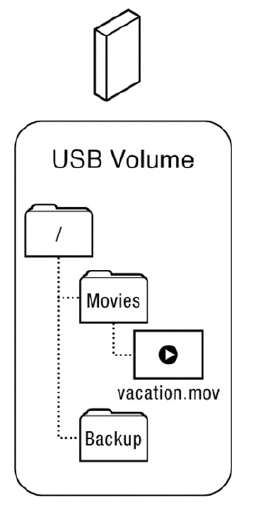
\includegraphics[scale=0.70]{img/fig1101}}
\caption{Este disco USB contiene un volumen que es el almacenamiento físico para un sistema de archivos.}
\label{fig1101}
\end{figure}

\begin{figure}[tbhp]
\centerline{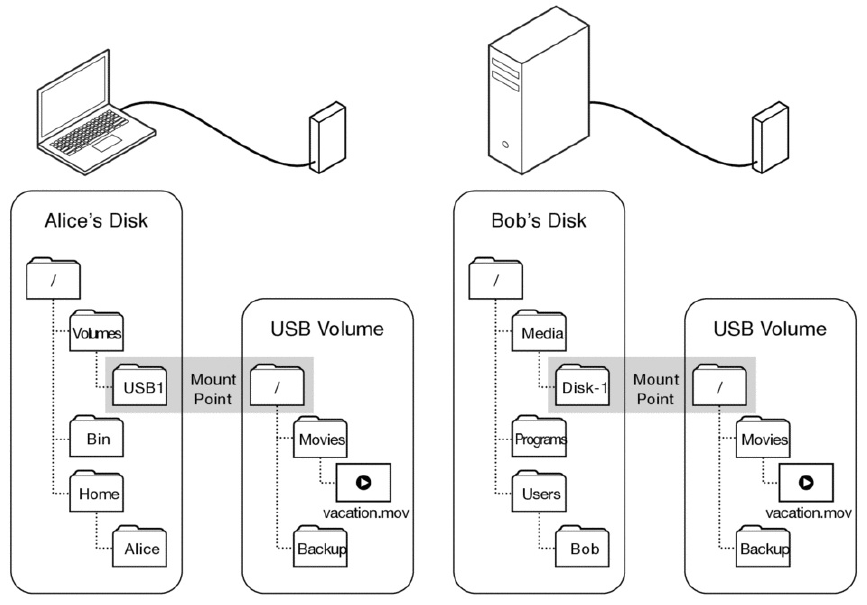
\includegraphics[scale=0.70]{img/fig1102}}
\caption{Un volumen puede montarse en otro sistema de archivos para unirse a sus jerarquías de directorios. Por ejemplo, cuando la unidad USB está conectada al ordenador de Alice, puede acceder a la película vacation.mov usando la ruta /Volumes/usb1/Movies/vacation.mov y cuando la unidad está conectada al ordenador de Bob, puede acceder a la película Utilizando la ruta /media/disk-1/Movies/vacation.mov.}
\label{fig1102}
\end{figure}

Por ejemplo, suponga que una unidad USB contiene un sistema de archivos con los directorios \textit{/Películas} y \textit{/Backup} como se muestra en la Figura \ref{fig1101}. Si Alice conecta esa unidad en su computadora portátil, el sistema operativo del portátil podría montar el sistema de archivos del volumen USB con la ruta \textit{/Volúmenes/usb1/} como se muestra en la Figura \ref{fig1102}. Luego, si Alice llama abierta \textit{/Volumes/usb1/Movies/vacation.mov}, abrirá el archivo \textit{/Movies/vacation.mov} del sistema de archivos en el volumen de la unidad USB. Si, en cambio, Bob se conecta a su computadora portátil, el sistema operativo del portátil podría montar el sistema de archivos del volumen con la ruta \textit{/media/disk-1}, y Bob accedería al mismo archivo usando la ruta \textit{/media/disk-1/Películas/Vacation.mov}.


\section{API}
\textbf{Creación y Eliminación de Archivos y Directorios.}

Los procesos crean y destruyen archivos con \textit{create()} y \textit{unlink()}. Create() hace dos cosas: crea un archivo nuevo que tiene metadatos iniciales pero no otros datos y crea un nombre para ese archivo en un directorio. \textit{Link()} crea un vínculo duro: un nuevo nombre de ruta para un archivo existente. Después de una llamada exitosa a \textit{link()}, hay varios nombres de ruta que se refieren al mismo archivo subyacente. \textit{Unlink()} elimina un nombre para un archivo de su directorio. Si un archivo tiene varios nombres o vínculos, \textit{unlink()} sólo elimina el nombre especificado, dejando el archivo accesible a través de otros nombres. Si el nombre especificado es el último (o único) vínculo a un archivo, entonces \textit{unlink()} también elimina el archivo subyacente y libera sus recursos. \textit{Mkdir()} y \textit{rmdir()} crean y eliminan directorios.

\textbf{Abrir y Cerrar.}

Para iniciar el acceso a un archivo, un proceso llama a \textit{open()} para obtener un descriptor de archivo que puede usar para referirse al archivo abierto. El descriptor de archivo es terminología de Unix; En otros sistemas el descriptor puede llamarse un identificador de archivo o un flujo de archivo.

Los sistemas operativos requieren procesos para abrir explícitamente los archivos y acceder a ellos a través de descriptores de archivos en lugar de simplemente pasar el nombre de la ruta de acceso a las llamadas \textit{read()} y \textit{write()} por dos razones. En primer lugar, el análisis de ruta y la comprobación de permisos pueden realizarse justo cuando se abre un archivo y no es necesario repetirlo en cada lectura o escritura. En segundo lugar, cuando un proceso abre un archivo, el sistema operativo crea una estructura de datos que almacena información sobre el archivo abierto del proceso, como el ID del archivo, si el proceso puede escribir o simplemente leer el archivo y un puntero a la posición actual del proceso dentro de el archivo. El descriptor de archivo puede considerarse así como una referencia a la estructura de datos del sistema operativo por archivo abierto que el sistema operativo utilizará para administrar el acceso del proceso al archivo.

Cuando una aplicación se realiza mediante un archivo, llama a \textit{close()}, que libera el registro de archivo abierto en el sistema operativo.

\textbf{Acceso a Archivos.}

Mientras un archivo está abierto, una aplicación puede acceder a los datos del archivo de dos maneras. En primer lugar, puede utilizar la interfaz de procedimiento tradicional, haciendo llamadas de sistema a \textit{read()} y \textit{write()} en un archivo abierto. Las llamadas a \textit{read()} y \textit{write()} comienzan desde la posición actual del archivo del proceso, y avanzan la posición del archivo actual por el número de bytes que se han leído o escrito correctamente. Por lo tanto, una secuencia de las llamadas \textit{read()} o \textit{write()} se mueve secuencialmente a través de un archivo. Para admitir acceso aleatorio dentro de un archivo, la llamada \textit{seek()} cambia la posición actual de un proceso para un archivo abierto especificado.

En lugar de usar \textit{read()} y \textit{write()} para acceder a los datos de un archivo, una aplicación puede usar \textit{mmap()} para establecer una correlación entre una región de la memoria virtual del proceso y alguna región del archivo. Una vez que se ha asignado un archivo, la memoria carga y almacena en esa región de memoria virtual leerá y escribirá los datos del archivo, ya sea accediendo a una página compartida desde la caché de archivos del kernel o activando una excepción de fallo de página que haga que el kernel busque el archivo deseado en la página de datos del sistema de archivos en la memoria. Cuando una aplicación se realiza con un archivo, puede llamar a \textit{munmap()} para eliminar las asignaciones.

Por último, la llamada \textit{fsync()} es importante para la confiabilidad. Cuando una aplicación actualiza un archivo a través de \textit{write()} o un almacén de memoria en un archivo asignado, las actualizaciones se guardan en memoria intermedia y se guardan en un almacenamiento estable en un futuro. \textit{Fsync()} garantiza que todas las actualizaciones pendientes de un archivo se escriban en almacenamiento persistente antes de que se devuelva la llamada. Las aplicaciones utilizan esta función para dos propósitos. En primer lugar, llamar a \textit{fsync()} asegura que las actualizaciones sean duraderas y no se perderán si hay un fallo del sistema o un fallo de energía. En segundo lugar, llamar a \textit{fsync()} entre dos actualizaciones asegura que la primera se escribe en el almacenamiento persistente antes de la segunda. Tenga en cuenta que llamar a \textit{fsync()} no siempre es necesario; El sistema operativo garantiza que todas las actualizaciones se hagan duraderas al limpiar periódicamente todos los bloques de archivos sucios a un almacenamiento estable.


\setcounter{chapter}{12}
\chapter{Archivos y directorios}
Recordemos que los sistemas de archivos utilizan directorios para proporcionar archivos nombrados de manera jerárquica y que cada archivo contiene \textbf{metadatos} y una secuencia de bytes de datos. Sin embargo, los dispositivos de almacenamiento proporcionan una abstracción de mucho menor nivel: grandes matrices de bloques de datos. Por lo tanto, para implementar un sistema de archivos, debemos resolver un problema de traducción: ¿Cómo vamos desde un nombre de archivo y desplazamiento a un número de bloque?

Una respuesta simple es que los sistemas de archivos implementan un diccionario que mapea claves (nombre de archivo y desplazamiento) a valores (número de bloque en un dispositivo). De todas formas, los diseñadores de sistemas de archivos se enfrentan a cuatro grandes desafíos:
\begin{itemize}
\item \textbf{Rendimiento}. Los sistemas de archivos deben mantener un buen rendimiento mientras realizan copias con las limitaciones relacionadas a los dispositivos de almacenamiento subyacentes. En la práctica, esto significa que los sistemas de archivos se esfuerzan por asegurar una buena \textit{localidad espacial}, donde los bloques que se acceden juntos se almacenan cerca uno de otro, idealmente en bloques de almacenamiento secuencial.
\item \textbf{Flexibilidad}. Uno de los principales objetivos de los sistemas de archivos es permitir que las aplicaciones compartan datos, por lo que los sistemas de archivos deben estar preparados para todo tipo de usos. Serían menos útiles si tuviéramos que usar un sistema de archivos para archivos grandes de lectura secuencial, otro para archivos pequeños rara vez escritos, otro para archivos grandes de acceso aleatorio, otro para archivos de corta duración, etc.
\item \textbf{Persistencia}. Los sistemas de archivos deben mantener y actualizar tanto los datos de usuario como sus estructuras internas de datos en los dispositivos de almacenamiento persistentes para que todo sobreviva a fallos del sistema operativo y a fallos de alimentación.
\item \textbf{Confiabilidad}. Los sistemas de archivos deben ser capaces de almacenar datos importantes durante largos períodos de tiempo, incluso si las máquinas se bloquean durante las actualizaciones o se produjeran fallas en el hardware de almacenamiento del sistema.
\end{itemize}

\section{Vistazo de la implementación}
Los sistemas de archivos deben asignar nombres de archivos y desplazamientos a bloques físicos de almacenamiento de manera que permitan un acceso eficiente. Aunque existen muchos sistemas de archivos diferentes, la mayoría de las implementaciones se basan en cuatro ideas clave: directorios, estructuras de índices, mapas de espacio libre y heurísticas de localidades.

\begin{figure}[tbhp]
\centerline{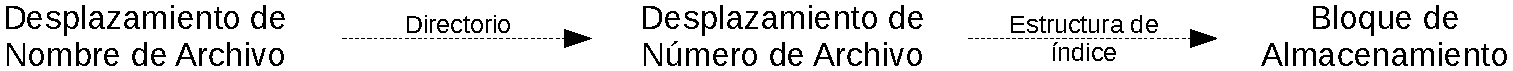
\includegraphics[scale=0.65]{img/fig1301}}
\caption{Los sistemas de archivos asignan nombres de archivos y desplazamientos de archivos a bloques de almacenamiento en dos pasos. En primer lugar, utilizan directorios para asignar nombres a números de archivo. A continuación, utilizan una estructura de índice como un árbol almacenado de forma persistente para encontrar el bloque que contiene los datos en cualquier desplazamiento específico en ese archivo.}
\label{fig1301}
\end{figure}

\textbf{Directorios y estructuras de índices}. Como se ilustra en la \textit{Fig.} \ref{fig1301}, los sistemas de archivos asignan nombres de archivos y conjuntos de archivos a bloques de almacenamiento específicos en dos pasos.

En primer lugar, utilizan directorios para asignar nombres de archivo legibles por humanos a números de archivo. Los directorios a menudo son sólo archivos especiales que contienen listas de asignaciones \textit{nombre de archivo} $\rightarrow$ \textit{número de archivo}.

En segundo lugar, una vez que un nombre de archivo se ha traducido a un número de archivo, los sistemas de archivos utilizan una estructura de índice almacenada de forma persistente para localizar los bloques del archivo. La estructura de índice puede ser cualquier estructura de datos persistente que asigna un número de archivo y un desplazamiento a un bloque de almacenamiento. A menudo, para soportar eficientemente una amplia gama de tamaños de archivo y patrones de acceso, la estructura de índice es una forma de árbol.

\textbf{Mapas de espacio libre}. Los sistemas de archivos implementan mapas de espacio libre para rastrear qué bloques de almacenamiento están libres y qué bloques están en uso a medida que los archivos crecen y se contraen. Como mínimo, el mapa de espacio libre del sistema de archivos debe permitir que éste encuentre un bloque libre cuando un archivo necesita crecer, pero debido a que la ubicación espacial es importante, la mayoría de los sistemas de archivos modernos implementan mapas de espacio libre que les permiten encontrar bloques libres cerca de una ubicación deseada. Por ejemplo, muchos sistemas de archivos implementan mapas de espacio libre como mapas de bits en almacenamiento persistente.

\textbf{Heurística de la localidad}. Los directorios y las estructuras de índices permiten a los sistemas de archivos localizar los datos de archivo y los metadatos deseados sin importar dónde se almacenen, y los mapas de espacio libre les permiten localizar el espacio libre cerca de cualquier ubicación del dispositivo de almacenamiento persistente. Estos mecanismos permiten a los sistemas de archivos emplear varias políticas para decidir dónde debe almacenarse un bloque dado de un archivo dado.

Estas políticas se materializan en \textit{heurísticas de localidad} para agrupar datos para optimizar el rendimiento. Por ejemplo, algunos sistemas de archivos agrupan los archivos de cada directorio, pero esparcen diferentes directorios a diferentes partes del dispositivo de almacenamiento. Otros desfragmentan periódicamente su almacenamiento, reescribiendo los archivos existentes para que cada archivo se almacene en bloques de almacenamiento secuencial y de modo que el dispositivo de almacenamiento tenga largas secuencias de espacio libre secuencial para que los nuevos archivos se puedan escribir secuencialmente. Y otros optimizan escrituras vs. lecturas, y escriben todos los datos secuencialmente, si un conjunto dado de escrituras contiene actualizaciones a un archivo o a muchos otros.

\section{Directorios: nombres de datos}
Como indica la \textit{Fig.} \ref{fig1301} para acceder a un archivo, el sistema de archivos traduce primero el nombre del archivo a su número. Por ejemplo, el archivo denominado {\mf /home/tom/foo.txt} puede conocerse internamente como archivo {\mf 66212871}. Los sistemas de archivos utilizan directorios para almacenar sus asignaciones de nombres legibles por humanos a números de archivos internos y organizan estos directorios de forma jerárquica para que los usuarios puedan agrupar Archivos relacionados y directorios.

\begin{figure}[tbhp]
\centerline{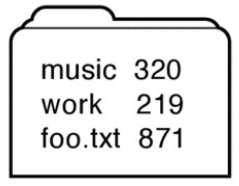
\includegraphics[scale=0.45]{img/fig1302}}
\caption{Un directorio es un archivo que contiene una colección de asignaciones (\textit{nombre de archivo} $\rightarrow$ \textit{número de archivo}).}
\label{fig1302}
\end{figure}

La implementación de directorios de una manera que proporciona mapeos jerárquicos de nombre a número resulta ser simple: se utilizan archivos para almacenar directorios. Por lo tanto, si el sistema necesita determinar el número de un archivo, sólo puede abrir el archivo de directorio apropiado y escanear a través de los pares (nombre de archivo/número de archivo) hasta encontrar el correcto.

Por ejemplo, la \textit{Fig.} \ref{fig1302} ilustra el contenido de un único archivo de directorio. Para abrir el archivo {\mf foo.txt}, el sistema de archivos analizará este archivo de directorio, encontrará la entrada {\mf foo.txt} y verá que el archivo {\mf foo.txt} tiene el número de archivo {\mf 66212871}.

\begin{figure}[tbhp]
\centerline{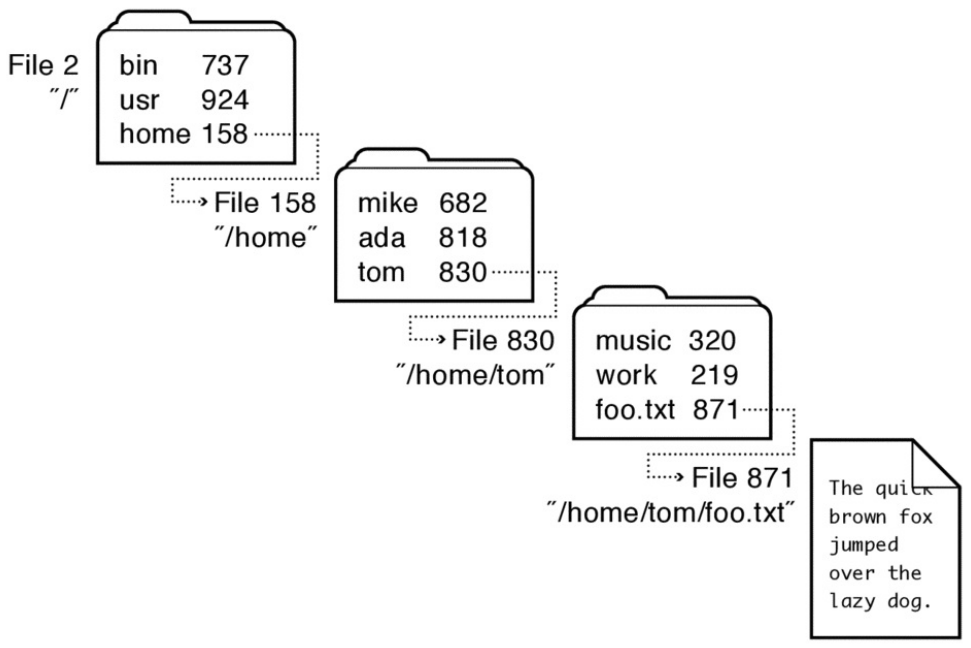
\includegraphics[scale=0.45]{img/fig1303}}
\caption{Los directorios pueden organizarse jerárquicamente al tener un directorio que contenga la asignación (\textit{nombre de archivo} $\rightarrow$ \textit{número de archivo}) para otro directorio.}
\label{fig1303}
\end{figure}

Por supuesto, si usamos archivos para almacenar el contenido de directorios como {\mf /home/tom}, todavía tenemos el problema de encontrar los archivos de directorio en sí. Como se muestra en la \textit{Fig.} \ref{fig1303}, el número de archivo del directorio {\mf /home/tom} se puede encontrar buscando el nombre {\mf tom} en el directorio {\mf /home} y el número de archivo para directorio {\mf /home} se puede buscar buscando el nombre {\mf home} en el directorio raíz {\mf /}.

Los algoritmos recursivos necesitan un caso base: no podemos descubrir el número de archivo de directorios raíz mirando en algún otro directorio. La solución es acordar el número de archivo del directorio raíz con antelación. Por ejemplo, el \textbf{Fast File System} (FFS) de Unix y muchos otros sistemas de archivos Unix y Linux usan {\mf 2} como el número de archivo predefinido para el directorio raíz de un sistema de archivos.

Por lo tanto, para leer el archivo {\mf /home/tom/foo.txt} en la \textit{Fig.} \ref{fig1303}, leemos primero el directorio raíz leyendo el archivo con la bien conocida raíz número {\mf 2}. En ese archivo, buscamos el nombre {\mf home} y encontramos que directorio {\mf /home} está almacenado en el archivo {\mf 88026158}. Leyendo el archivo {\mf 88026158} y buscando el nombre {\mf tom}, aprendemos que directorio {\mf /home/tom} está almacenado en el archivo {\mf 5268830}. Finalmente, por Leyendo archivo {\mf 5268830} y buscando el nombre {\mf foo.txt}, nos enteramos de que {\mf /home/tom/foo.txt} es el número de archivo {\mf 66212871}.

Aunque buscar el número de un archivo puede tomar varios pasos, esperamos que haya localidad (por ejemplo, cuando se accede a un archivo en un directorio, es muy probable que pronto se acceda a otros archivos del mismo directorio), por lo que esperamos que el almacenamiento en caché reduzca el número de accesos de disco necesarios para la mayoría de las búsquedas.

\textbf{API de directorios}. Los directorios utilizan una API especializada porque deben controlar el contenido de estos archivos. Por ejemplo, los sistemas de archivos deben evitar que las aplicaciones corrompan la lista de asignaciones (\textit{nombre de archivo} $\rightarrow$ \textit{número de archivo}), lo que podría impedir que el sistema operativo realice búsquedas o actualizaciones. Como otro ejemplo, el sistema de archivos debe hacer cumplir el invariante de que cada número de archivo en una entrada de directorio válida se refiere a un archivo que realmente existe.

Por lo tanto, los sistemas de archivos proporcionan llamadas especiales al sistema para modificar los archivos de directorio. Por ejemplo, en lugar de utilizar la llamada de sistema de escritura estándar para agregar una entrada de un nuevo archivo a un directorio, las aplicaciones utilizan la llamada {\mf create}. Al restringir las actualizaciones, estas llamadas garantizan que los archivos de directorio siempre pueden ser analizados por el sistema operativo. Estas llamadas también enlazan la creación o eliminación de un archivo y la entrada de directorio del archivo, de modo que las entradas de directorio siempre se refieren a archivos reales y que todos los archivos tienen al menos una entrada de directorio.

\textbf{Detalles internos de los directorios}. Muchas de las primeras implementaciones de sistemas de archivos simplemente almacenaban listas lineales de pares (nombre de archivo/número de archivo) en archivos de directorio. Por ejemplo, en la versión original del sistema de archivos ext2 de Linux, cada archivo de directorio almacenaba una lista vinculada de entradas de directorio como se ilustra en la \textit{Fig.} \ref{fig1304}.

\begin{figure}[tbhp]
\centerline{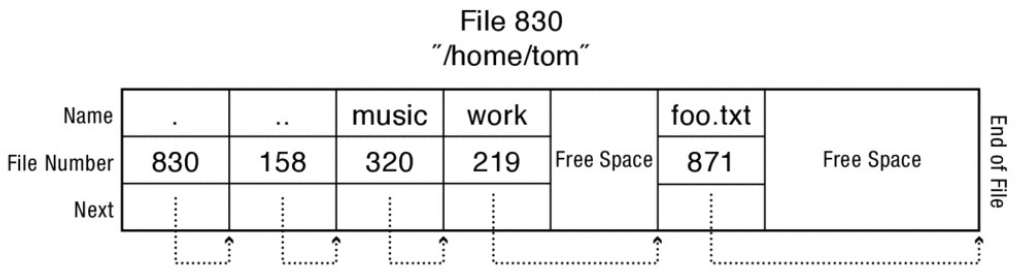
\includegraphics[scale=0.50]{img/fig1304}}
\caption{Una implementación de lista vinculada de un directorio. Este ejemplo muestra un archivo de directorio que contiene cinco entradas: {\mf music}, {\mf work} y {\mf foo.txt}, junto con {\mf .} (el directorio actual) y {\mf ..} (el directorio padre).}
\label{fig1304}
\end{figure}

Las listas simples funcionan bien cuando el número de entradas de directorio es pequeño. Una vez que un directorio tiene unos pocos miles de entradas, los directorios basados en listas simples se vuelven lentos.

Para soportar de forma eficaz directorios con muchas entradas, muchos sistemas de archivos recientes, incluyendo XFS de Linux y NTFS de Microsoft, entre otros, aumentan la lista vinculada subyacente con una estructura adicional basada en hash para acelerar las búsquedas. Estos sistemas de archivos implementan registros de directorio que mapean nombres de archivo a números de archivo y dichas asignaciones se almacenan en un \textbf{árbol B+} indexado por el hash del nombre de cada archivo. Para encontrar el número de archivo de un nombre de archivo dado, el sistema de archivos calcula primero un hash del nombre. A continuación, utiliza ese hash como clave para buscar la entrada del directorio en el árbol: comenzando en la raíz del árbol B+ en un desplazamiento bien conocido en el archivo y procediendo a través de los nodos internos hacia los nodos hoja del árbol. En cada nivel, un nodo contiene una matriz de pares (clave de hash/desplazamiento de archivo) que representan cada uno un puntero al nodo secundario que contiene entradas con claves más pequeñas que la clave de hash pero mayores que la clave de hash de la entrada anterior. El sistema de archivos busca en el nodo la primera entrada con un valor de clave de hash que excede la clave de destino y, a continuación, sigue el puntero de desplazamiento de archivo correspondiente al nodo secundario correcto. El puntero de desplazamiento de archivo en el registro en los nodos hoja apunta a la entrada de directorio de destino.

\textbf{Hard y soft links}. Muchos sistemas de archivos permiten que un archivo dado tenga varios nombres. Los \textbf{hard links} o enlaces duros son varias entradas de directorio de archivos que asignan nombres de ruta diferentes al mismo número de archivo. Debido a que un número de archivo puede aparecer en varios directorios, los sistemas de archivos deben asegurarse de que un archivo sólo se elimina cuando se ha eliminado el último hard link.

Para implementar correctamente la recolección de basura, los sistemas de archivos usan recuentos de referencia almacenando con cada archivo el número de enlaces duros a él. Cuando se crea un archivo, tiene un recuento de referencia de uno, y cada enlace duro adicional hecho al archivo incrementa su recuento de referencias. Por el contrario, cada llamada a desvincular disminuye el recuento de referencia del archivo y cuando el recuento de referencia cae a cero, el archivo subyacente se elimina y sus recursos se marcan como libres.

Por otra parte, en lugar de asignar un nombre de archivo a un número de archivo, los \textbf{soft links} o enlaces simbólicos son entradas de directorio que asignan un nombre a otro nombre.

\begin{figure}[tbhp]
\centerline{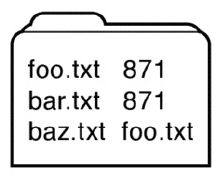
\includegraphics[scale=0.50]{img/fig1305}}
\caption{En este directorio, los hard links {\mf foo.txt} y {\mf bar.txt} y el soft link {\mf baz.txt} se refieren todos al mismo archivo.}
\label{fig1305}
\end{figure}

Por ejemplo, \textit{Fig.} \ref{fig1305} muestra un directorio que contiene tres nombres y todos se refieren al mismo archivo. Las entradas {\mf foo.txt} y {\mf bar.txt} son enlaces duros con el mismo archivo (número 66212871); {\mf baz.txt} es un enlace suave a {\mf foo.txt}. Debe notarse que si eliminamos la entrada {\mf foo.txt} de este directorio utilizando la llamada de sistema de desvinculación, el archivo todavía se puede abrir con el nombre {\mf bar.txt}, pero si intentamos abrirlo con el nombre {\mf baz.txt}, el intento fallará.


\section{Archivos: Búsqueda de datos}
Una vez que un sistema de archivos ha traducido un nombre de archivo a un número de archivo utilizando un directorio, el sistema de archivos debe ser capaz de encontrar los bloques que pertenecen a ese archivo. Además de este requisito funcional, las implementaciones de archivos suelen tener como objetivo otros cinco objetivos:
\begin{itemize}
\item Soportar la colocación secuencial de datos para maximizar el acceso secuencial a archivos.
\item Proporcionar acceso aleatorio eficiente a cualquier bloque de archivos.
\item Limitar las cargas de sistema (\textit{overheads}) para ser eficiente para archivos pequeños.
\item Ser escalable para admitir archivos grandes.
\item Proporcionar un lugar para almacenar metadatos por archivo, como el número de referencia del archivo, el propietario, la lista de control de acceso, el tamaño y el tiempo de acceso.
\end{itemize}

\subsection{FAT: Lista enlazada}
El sistema de archivos \textbf{FAT -- File Allocation Table} de Microsoft (Tabla de Asignación de Archivos) se implementó por primera vez a finales de los años setenta y era el sistema de archivos principal para MS-DOS y las primeras versiones de Microsoft Windows. El sistema de archivos FAT se ha mejorado de muchas maneras a lo largo de los años. La versión FAT-32 soporta volúmenes con hasta $2^{28}$ bloques y archivos con hasta $2^{32} - 1$ bytes.

\textbf{Estructuras de índices}. El sistema de archivos FAT recibe el nombre de su tabla de asignación de archivos, una matriz de entradas de 32 bits en un área reservada del volumen. Cada archivo del sistema corresponde a una lista vinculada de entradas FAT, con cada entrada FAT conteniendo un puntero a la siguiente entrada FAT del archivo (o un valor especial de ``fin de archivo''). La FAT tiene una entrada para cada bloque en el volumen y los bloques del archivo son los bloques que corresponden a las entradas FAT del archivo: si la entrada FAT i es la entrada i-ésima de un archivo, entonces el bloque de almacenamiento i es el i-ésimo bloque de datos del archivo.

\begin{figure}[tbhp]
\centerline{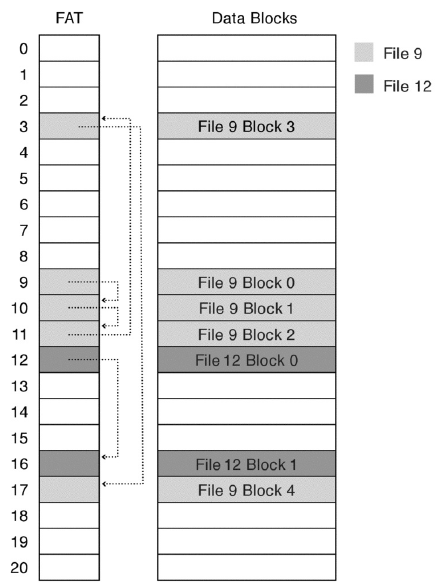
\includegraphics[scale=0.65]{img/fig1306}}
\caption{Un sistema de archivos FAT con un archivo de 5 bloques y un archivo de 2 bloques.}
\label{fig1306}
\end{figure}

La \textit{Fig.} \ref{fig1306} ilustra un sistema de archivos FAT con dos archivos. La primera comienza en el bloque {\mf 9} y contiene cinco bloques. El segundo comienza en el bloque {\mf 12} y contiene dos bloques.

Los directorios asignan nombres de archivo a números de archivo y, en el sistema de archivos FAT, el número de un archivo es el índice de la primera entrada del archivo en el FAT. Por lo tanto, dado el número de un archivo, podemos encontrar la primera entrada FAT y el bloque de un archivo, y dada la primera entrada FAT, podemos encontrar el resto de las entradas y bloques FAT del archivo.

\textbf{Seguimiento de espacio libre}. FAT también se utiliza para el seguimiento de espacio libre. Si el bloque de datos i está libre, entonces FAT[i] contiene un 0. Así, el sistema de archivos puede encontrar un bloque libre escaneando a través de la FAT para encontrar una entrada cero.

\textbf{Heurística de localidad}. Diferentes implementaciones de FAT pueden utilizar diferentes estrategias de asignación, pero las estrategias de asignación de implementaciones de FAT son generalmente simples. Por ejemplo, algunas implementaciones utilizan un algoritmo de ajuste siguiente (\textit{next fit}) que escanea secuencialmente a través de la FAT a partir de la última entrada asignada y que devuelve la siguiente entrada libre encontrada.

Estrategias de asignación simples como ésta pueden fragmentar un archivo, extendiendo los bloques del archivo a través del volumen en lugar de lograr el diseño secuencial deseado. Para mejorar el rendimiento, los usuarios pueden ejecutar una herramienta de \textbf{desfragmentación} que lee archivos de sus ubicaciones existentes y los vuelve a escribir a nuevas ubicaciones con una mejor localidad espacial. El desfragmentador FAT en Windows XP, por ejemplo, intenta copiar los bloques de cada archivo que se extiende a través de múltiples extensiones a una extensión secuencial única que contiene todos los bloques de un archivo.

\textbf{Usos y limitaciones}. El sistema de archivos FAT se utiliza ampliamente porque es simple y compatible con muchos sistemas operativos. Por ejemplo, muchas dispositivos de almacenamiento flash  USB y tarjetas de almacenamiento de cámaras utilizan el sistema de archivos FAT, permitiendo que sean leídos y escritos por casi cualquier computadora que ejecute casi cualquier sistema operativo moderno.

El sistema de archivos FAT, sin embargo, está limitado de muchas maneras. Por ejemplo,
\begin{itemize}
\item \textbf{Pobre empleo de la localidad}. Las implementaciones de FAT suelen utilizar estrategias de asignación sencillas, como el ajuste siguiente ya descrito. Estos pueden conducir a archivos mal fragmentados.
\item \textbf{Acceso aleatorio deficiente}. El acceso aleatorio dentro de un archivo requiere el desplazamiento secuencial de las entradas FAT del archivo hasta que se alcance el bloque deseado.
\item \textbf{Metadatos limitados de archivos y control de acceso}. Los metadatos de cada archivo incluyen información como el nombre, el tamaño y el tiempo de creación del archivo, pero no incluyen información de control de acceso, como el propietario del archivo o el ID de grupo, para que cualquier usuario pueda leer o escribir cualquier archivo almacenado en un sistema de archivos FAT.
\item \textbf{No hay soporte para enlaces duros}. FAT representa cada archivo como una lista vinculada de entradas de 32 bits en la tabla de asignación de archivos. Esta representación no incluye espacio para otros metadatos de archivo. En su lugar, los metadatos de archivo son almacenados como entradas de directorio con el nombre del archivo. Este enfoque exige que cada archivo se acceda a través de una entrada de directorio exactamente, descartando múltiples enlaces duros a un archivo.
\item \textbf{Limitaciones en volumen y tamaño de archivo}. Las entradas de tabla FAT son de 32 bits, pero los cuatro bits superiores se encuentran reservados. Así, un volumen FAT puede tener como máximo $2^{28}$ bloques. Con bloques de 4 KB, el tamaño máximo de volumen está limitado (por ejemplo, $2^{28} \frac{\text{bloques}}{\text{volumen}} \times 2^{12}\frac{\text{bytes}}{\text{bloque}} = 2^{40}\frac{\text{bytes}}{\text{volumen}} =$ 1 TB). Se admiten bloques de hasta 256 KB, pero se corre el riesgo de perder grandes cantidades de espacio en disco debido a la fragmentación interna. Del mismo modo, los tamaños de archivo se codifican en 32 bits, por lo que ningún archivo puede ser mayor que $2^{32} - 1$ bytes (poco menos de 4 GB).
\item \textbf{Falta de soporte para técnicas modernas de confiabilidad}. FAT no admite las técnicas de actualización transaccional que
los sistemas de archivos modernos utilizan para evitar la corrupción de las estructuras de datos críticos si el equipo se bloquea mientras se escribe en el almacenamiento.
\end{itemize}


\subsection{FFS: Árbol fijo}
El \textbf{Sistema de Archivos Rápido} de Unix (FFS: \textit{Fast File System}) ilustra ideas importantes para la indexación de los bloques de un archivo para que puedan localizarse rápidamente y para colocar los datos en el disco para obtener una buena localidad. En particular, la estructura de índice de FFS, denominada índice multinivel, es un árbol cuidadosamente estructurado que permite a FFS localizar cualquier bloque de un archivo y que es eficiente tanto para archivos grandes como pequeños. Dada la flexibilidad proporcionada por el índice de niveles múltiples de FFS, FFS emplea dos heurísticas de localidad -- colocación de grupo de bloque y espacio de reserva -- que juntas suelen proporcionar un buen diseño en disco.

\textbf{Estructuras de índices}. Para realizar un seguimiento de los bloques de datos que pertenecen a cada archivo, FFS utiliza un árbol asimétrico fijo denominado \textbf{índice multinivel}, como se ilustra en la \textit{Fig.} \ref{fig1307}.

\begin{figure}[tbhp]
\centerline{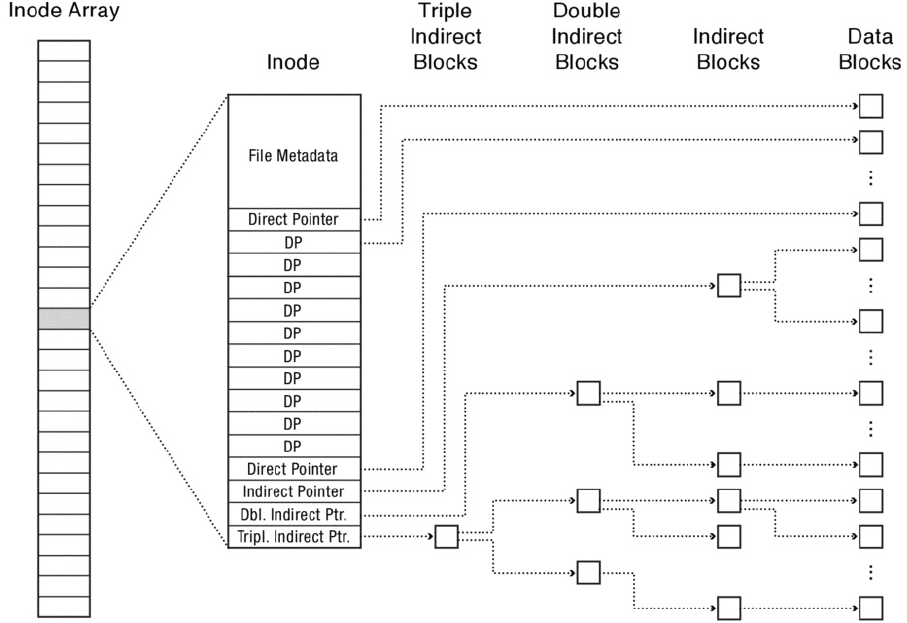
\includegraphics[scale=0.65]{img/fig1307}}
\caption{Un inodo FFS es la raíz de un árbol asimétrico cuyas hojas son los bloques de datos de un archivo.}
\label{fig1307}
\end{figure}

Cada archivo es un árbol con bloques de datos de tamaño fijo (por ejemplo, 4 KB) como sus hojas. El árbol de cada archivo está enraizado en un \textbf{inodo} que contiene los metadatos del archivo (por ejemplo, el propietario del archivo, los permisos de control de acceso, la hora de creación, la última hora modificada y si el archivo es un directorio o no). 

El inodo de un archivo (raíz) también contiene una matriz de punteros para localizar los bloques de datos (hojas) del archivo. Algunos de estos punteros apuntan directamente a las hojas de datos del árbol y algunos apuntan a nodos internos en el árbol. Típicamente, un inodo contiene 15 punteros. Los primeros 12 punteros son \textbf{punteros directos} que apuntan directamente a los primeros 12 bloques de datos de un archivo.

El puntero 13 es un \textbf{puntero indirecto}, que apunta a un nodo interno del árbol llamado \textbf{bloque indirecto}. Un bloque indirecto es un bloque regular de almacenamiento que contiene una matriz de punteros directos. Para leer el bloque 13 de un archivo, primero lee el inodo para obtener el puntero indirecto, luego el bloque indirecto para obtener el puntero directo, luego el bloque de datos. Con bloques de 4 KB y punteros de bloques de 4 bytes, un bloque indirecto puede contener hasta 1024 punteros directos, lo que permite archivos de hasta poco más de 4 MB.

El puntero 14 es un \textbf{doble puntero indirecto}, que apunta a un nodo interno del árbol llamado \textbf{doble bloque indirecto}. Un doble bloque indirecto es una matriz de indicadores indirectos, cada uno de los cuales apunta a un bloque indirecto. Con bloques de 4 KB y punteros de bloques de 4 bytes, un bloque indirecto doble puede contener hasta 1024 punteros indirectos. Así, un puntero indirecto doble puede indexar tantos como $1024^2$ bloques de datos.

Finalmente, el puntero 15 es un \textbf{puntero triple indirecto} que apunta a un \textbf{bloque indirecto triple} que contiene una matriz de punteros indirectos dobles. Con un bloque de 4 KB y un indicador de bloque de 4 bytes, un puntero indirecto triple puede indexar hasta $1024^3$ bloques de datos que contienen $4\text{ KB}\times 1024^3 = 2^{12} \times 2^{30} = 2^{42}$ bytes (4 TB).

Todos los inodos de un sistema de archivos se encuentran en una matriz de inodos que se almacena en una ubicación fija en el disco. El número de archivo de un archivo, denominado \textbf{inúmero} (\textit{inumber}) en FFS, es un índice en la matriz inodo: para abrir un archivo (por ejemplo, {\mf foo.txt}), buscamos en el directorio del archivo para encontrar su número (por ejemplo, {\mf 91854}) y luego buscamos la entrada apropiada de la matriz de inodos (por ejemplo, la entrada {\mf 91854}) para encontrar sus metadatos.

El índice multinivel de FFS tiene cuatro características importantes:
\begin{enumerate}
\item \textbf{Estructura del árbol}. Cada archivo se representa como un árbol, lo que permite al sistema de archivos encontrar eficientemente cualquier bloque de un archivo.
\item \textbf{Alto grado}. El árbol FFS utiliza nodos internos con muchos hijos en comparación con los árboles binarios que se usan con frecuencia para estructuras de datos en memoria. Por ejemplo, si un bloque de archivo es de 4 KB y un bloque de ID es de 4 bytes, cada bloque indirecto puede contener punteros a 1024 bloques.

Los nodos de alto grado tienen sentido para las estructuras de datos en disco donde (1) queremos minimizar el número de búsquedas, (2) el costo de leer varios kilobytes de datos secuenciales no es mucho mayor que el costo de leer el primer byte y (3) los datos deben ser leídos y escritos por lo menos un sector a la vez. Los nodos de alto grado también mejoran la eficiencia de lecturas y escrituras secuenciales. Una vez leído un bloque indirecto, se pueden leer cientos de bloques de datos antes de que se necesite el siguiente bloque indirecto. Las corridas entre las lecturas de bloques indirectos dobles son aún mayores.

\item \textbf{Estructura fija}. El árbol FFS tiene una estructura fija. Para una configuración dada de FFS, el primer conjunto de {\mf d} punteros apunta siempre a los primeros {\mf d} bloques de un archivo; El siguiente puntero es un puntero indirecto que apunta a un bloque indirecto, etc. En comparación con un árbol dinámico que puede añadir capas de indirección por encima de un bloque a medida que crece un archivo, la principal ventaja de la estructura fija es la simplicidad de implementación.

\item \textbf{Asimétrico}. Para soportar eficientemente archivos grandes y pequeños con una estructura de árbol fija, la estructura de árbol de FFS es asimétrica. En lugar de poner cada bloque de datos a la misma profundidad, FFS almacena sucesivos grupos de bloques a mayor profundidad para que los archivos pequeños se almacenen en un árbol de poca profundidad, la mayor parte de los archivos medianos se almacenan en un árbol de profundidad media y el volumen De los archivos grandes se almacenan en un árbol de mayor profundidad. Por ejemplo, un pequeño archivo de 4 bloques cuyo inodo incluye punteros directos a todos sus bloques. Por el contrario, para el archivo grande mostrado en la \textit{Fig.} \ref{fig1307}, la mayoría de los bloques deben ser accedidos a través del triple puntero indirecto.

Por el contrario, si usamos un árbol de profundidad fija y queremos soportar archivos razonablemente grandes, los archivos pequeños pagarían altas sobrecargas (\textit{overheads}). Con punteros indirectos triples y bloques de 4 KB, almacenar un archivo de 4 KB consumiría más de 16 KB (el 4 KB de datos, el pequeño inodo y 3 niveles de bloques indirectos de 4 KB) y leer el archivo requeriría leer cinco bloques para atravesar el árbol.
\end{enumerate}

\textbf{Control de acceso FFS}. El inodo FFS contiene información para controlar el acceso a un archivo. El control de acceso se puede especificar para tres grupos de personas:
\begin{itemize}
\item \textbf{Usuario} (propietario). El usuario propietario del archivo.
\item \textbf{Grupo}. Conjunto de personas pertenecientes a un grupo Unix especificado. Cada grupo Unix se especifica en otro lugar como un nombre de grupo y una lista de usuarios en ese grupo.
\item \textbf{Otro}. Todos los demás usuarios.
\end{itemize}

El control de acceso se especifica en términos de tres tipos de actividades:
\begin{itemize}
\item \textbf{Leer}. Leer el archivo o directorio normal.
\item \textbf{Escribir}. Modificar el archivo o directorio normal.
\item \textbf{Ejecutar}. Ejecutar el archivo normal o recorrer el directorio para acceder a archivos o subdirectorios en él.
\end{itemize}

El inodo de cada archivo almacena las identidades del usuario (propietario) y grupo del archivo, así como 9 bits básicos de control de acceso para especificar el permiso de lectura / escritura / ejecución para el usuario del archivo (propietario) / grupo / otro. Por ejemplo, el comando {\mf ls -ld /} muestra la información de control de acceso para el directorio raíz:

\begin{lstlisting}[style=Bash,numbers=none]
> ls -ld /
drwxr-xr-x 40 root wheel 1428 Feb 2 13:39 /
\end{lstlisting}

Esto significa que el archivo es un directorio ({\mf d}), propiedad del usuario {\mf root} del grupo {\mf wheel}. El directorio raíz puede ser leído, escrito y ejecutado (recorrido) por el propietario ({\mf rwx}), y puede ser leído y ejecutado (recorrido) pero no escrito por los miembros del grupo {\mf wheel} ({\mf r-x}) y todos los demás usuarios ({\mf r-x}).

\textbf{Los programas setuid y setgid}. Además de los 9 bits de control de acceso básicos, el inodo FFS almacena dos bits adicionales importantes:
\begin{itemize}
\item \textbf{setuid}. Cuando este archivo es ejecutado por cualquier usuario (con permiso de ejecución) se ejecutará con el permiso del propietario del archivo (en lugar del usuario). Por ejemplo, el programa {\mf lprm} permite al usuario eliminar un trabajo de una cola de impresión. La cola de impresión se implementa como un directorio que contiene los archivos que se van a imprimir, y porque no queremos que los usuarios puedan eliminar trabajos de otros usuarios, este directorio es propiedad del usuario {\mf root} y sólo puede ser modificado por él. Por lo tanto, el programa {\mf lprm} es propiedad del usuario {\mf root} con el bit {\mf setuid} establecido. Puede ser ejecutado por cualquier persona, pero cuando se ejecuta, se ejecuta con permisos de {\mf root}, lo que le permite modificar el directorio de la cola de impresión.4

Por supuesto, hacer un programa {\mf setuid} es potencialmente peligroso. Aquí, por ejemplo, confiamos en el programa {\mf lprm} para verificar que el usuario real está eliminando sus propios trabajos de impresión, no de otra persona. Un error en el programa {\mf lprm} podría permitir a un usuario eliminar los trabajos de otra impresora. Peor aún, si el error permite al atacante ejecutar código malicioso (por ejemplo, a través de un ataque de desbordamiento de búfer), un error en {\mf lprm} podría dar al atacante un control total de la máquina.

\item \textbf{setgid}. El bit {\mf setgid} es similar al bit {\mf setuid}, excepto que el archivo se ejecuta con el permiso de grupo del archivo. Por ejemplo, en algunas máquinas, {\mf sendmail} se ejecuta como miembro del grupo {\mf smmsp} para que pueda acceder a un archivo de cola de correo accesible al grupo {\mf smmsp}.
\end{itemize}

\textbf{Archivos dispersos (sparse)}. Las estructuras de índices basadas en árboles como las FFS pueden admitir archivos dispersos en los que uno o más rangos de espacio vacío están rodeados por datos de archivo. Los rangos de espacio vacío no consumen espacio en disco. Por ejemplo, si creamos un nuevo archivo, escribimos 4 KB en el desplazamiento 0 con un puntero directo, buscamos el desplazamiento 230 y escribimos otro 4 KB con un doble puntero indirecto. Luego, un sistema FFS con bloques de 4 KB sólo consumirá 16 KB: dos bloques de datos, un bloque indirecto doble y un solo bloque indirecto. En este caso, si listamos el tamaño del archivo usando el comando {\mf ls}, vemos que el tamaño del archivo es 1.1 GB. Pero, si comprobamos el espacio consumido por el archivo, usando el comando {\mf du}, vemos que consume sólo 16 KB de espacio de almacenamiento.

El soporte eficiente de archivos dispersos es útil para dar a las aplicaciones la máxima flexibilidad para colocar datos en un archivo. Por ejemplo, una base de datos podría almacenar sus tablas al comienzo de su archivo, sus índices en 1 GB en el archivo, su registro en 2 GB y metadatos adicionales a 4 GB.

Los archivos dispersos tienen dos limitaciones importantes. En primer lugar, no todos los sistemas de archivos los soportan, por lo que una aplicación que depende de soporte de archivos dispersos no puede ser portátil. En segundo lugar, no todas las utilidades manejan correctamente los archivos dispersos, lo que puede llevar a consecuencias inesperadas.

\textbf{Gestión del espacio libre}. La gestión del espacio libre de FFS es simple. FFS asigna un mapa de bits con un bit por bloque de almacenamiento. El i-ésimo bit en el mapa de bits indica si el i-ésimo bloque está libre o en uso. La posición del mapa de bits de FFS se fija cuando se formatea el sistema de archivos, por lo que es fácil encontrar la parte del mapa de bits que identifica bloques libres cerca de cualquier ubicación de interés.

\textbf{Heurística de localidad}. FFS utiliza dos heurísticas de localidad importantes para obtener un buen rendimiento para muchas cargas de trabajo:
\begin{itemize}
\item \textbf{Colocación de grupo de bloque}. FFS coloca los datos para optimizar el caso común en el que se accede a los bloques de datos de un archivo, a los datos y metadatos de un archivo y a diferentes archivos del mismo directorio. Por el contrario, debido a que todo no puede estar cerca de todo, FFS permite que los archivos de diferentes directorios estén lejos uno del otro. Esta heurística de colocación tiene cuatro partes:
\begin{enumerate}
\item \textbf{Dividir el disco en grupos de bloques}. FFS divide un disco en conjuntos de pistas cercanas llamadas grupos de bloques. El tiempo de búsqueda entre los bloques de un grupo de bloques será pequeño.
\item \textbf{Distribuir metadatos}. En FFS, la matriz de inodos y el mapa de bits de espacio libre siguen siendo conceptualmente matrices de registros y FFS aún almacena cada entrada de matriz en una ubicación bien conocida y fácilmente calculable, pero la matriz ahora se divide en piezas distribuidas a través del disco. En particular, cada grupo de bloques tiene una parte de estas estructuras de metadatos.
\item \textbf{Colocar el archivo en el grupo de bloques}. FFS coloca un directorio y sus archivos en el mismo grupo de bloques: cuando se crea un nuevo archivo, FFS conoce el número del directorio del nuevo archivo y desde ese punto puede determinar el rango de números en el mismo grupo de bloques. FFS elige un inodo de ese grupo si uno está libre; De lo contrario, FFS abandona la localidad y selecciona un número de un grupo de bloques diferente. En contraste con los archivos regulares, cuando FFS crea un nuevo directorio, elige un inúmero de un grupo de bloques diferente. Aunque podríamos esperar un subdirectorio para tener alguna localidad con su padre, poner todos los subdirectorios en el mismo grupo de bloques rápidamente lo llenaría, frustrando nuestros esfuerzos para conseguir la localidad dentro de un directorio.
\item \textbf{Colocar los bloques de datos}. Dentro de un grupo de bloques, FFS utiliza una primera heurística libre. Cuando se escribe un nuevo bloque de un archivo, FFS escribe el bloque en el primer bloque libre del grupo de bloques del archivo. Aunque esta heurística puede dejar de lado la localidad en el corto plazo, lo hace para mejorar la localidad a largo plazo. En el corto plazo, esta heurística podría extender una secuencia de escrituras en pequeños agujeros cerca del comienzo de un grupo de bloques en lugar de concentrarlos en una secuencia de bloques libres contiguos en algún otro lugar. Sin embargo, este sacrificio a corto plazo trae beneficios a largo plazo: la fragmentación se reduce, el bloque tiende a tener un largo plazo de espacio libre al final, las escrituras posteriores tienen más probabilidades de ser secuenciales.

La intuición es que un grupo de bloques dado normalmente tendrá un puñado de agujeros esparcidos a través de bloques cerca del inicio del grupo y una gran cantidad de espacio libre al final del grupo. Entonces, si se crea un archivo pequeño, sus bloques probablemente irán a algunos de los pequeños agujeros, lo cual no es ideal, pero es aceptable para un archivo pequeño. Por el contrario, si se crea un archivo grande y se escribe desde el principio hasta el final, tenderá a que los primeros bloques se dispersen a través de los orificios en la primera parte del bloque, pero luego se tiene la mayor parte de los datos escritos secuencialmente al final del grupo de bloques.

Si un grupo de bloques se queda sin bloques libres, FFS selecciona otro grupo de bloques y asigna bloques allí usando la misma heurística.
\end{enumerate}

\item \textbf{Espacio reservado}. Aunque la heurística de grupos de bloques puede ser efectiva, se basa en que existe una cantidad significativa de espacio libre en el disco. En particular, cuando un disco está casi lleno, hay poca oportunidad para que el sistema de archivos optimice la localidad. Por ejemplo, si un disco tiene sólo unos pocos kilobytes de sectores libres, la mayoría de los grupos de bloques estarán llenos y otros tendrán sólo unos cuantos bloques libres. Las nuevas escrituras tendrán que ser dispersas más o menos al azar por todo el disco.

FFS por lo tanto, reserva una parte del espacio del disco (por ejemplo, 10\%) y presenta un tamaño de disco ligeramente reducido a las aplicaciones. Si el espacio libre real en el disco cae por debajo de la fracción de reserva, FFS trata el disco como lleno. Por ejemplo, si la aplicación de un usuario intenta escribir un nuevo bloque en un archivo cuando se consuma todo menos el espacio de reserva, esa escritura fallará. Cuando todo, excepto el espacio de reserva está lleno, los procesos del superusuario seguirán siendo capaces de asignar nuevos bloques, lo cual es útil para permitir que un administrador inicie sesión y limpie las cosas.

El enfoque de Espacio reservado funciona bien teniendo en cuenta las tendencias en tecnología de discos. Se sacrifica una pequeña cantidad de capacidad de disco, un recurso de hardware que ha estado mejorando rápidamente en las últimas décadas, y reducir tiempos de búsqueda, una propiedad de hardware que ha mejorando más lentamente.
\end{itemize}


\subsection{NTFS: árbol flexible con extensiones}
El Sistema de Archivos de Nueva Tecnología de Microsoft (NTFS: \textit{New Technology File System}), lanzado en 1993, mejoró el sistema de archivos FAT de Microsoft con muchas nuevas características, incluyendo nuevas estructuras de índice para mejorar el rendimiento, metadatos de archivos más flexibles, mayor seguridad y mayor confiabilidad.

\textbf{Estructuras de índices}. Mientras que FFS rastrea los bloques de archivos con un árbol fijo, NTFS y muchos otros sistemas de archivos recientes, tales como ext4 de Linux, rastrean extensiones con \textit{árboles flexibles}.
\begin{itemize}
\item \textbf{Extensiones}. En lugar de rastrear bloques de archivos individuales, NTFS rastrea extensiones, regiones de tamaño variable de archivos que se almacenan cada una en una región contigua en el dispositivo de almacenamiento.
\item \textbf{Árbol flexible y tabla maestra de archivos}. Cada archivo en NTFS está representado por un árbol de profundidad variable. Los punteros de extensión para un archivo con un pequeño número de extensiones se pueden almacenar en un árbol superficial, incluso si el archivo, en sí mismo, es grande. Los árboles más profundos sólo son necesarios si el archivo se vuelve muy fragmentado.
\end{itemize}

Las raíces de estos árboles se almacenan en una tabla de archivos maestros que es similar a la matriz de inodos de FFS. La tabla de archivos maestros (MFT: \textit{Master File Table}) de NTFS almacena una matriz de registros MFT de 1 KB, cada uno de los cuales almacena una secuencia de registros de atributos de tamaño variable. NTFS utiliza registros de atributos para almacenar datos y metadatos, ambos son considerados atributos de un archivo.

Algunos atributos pueden ser demasiado grandes para encajar en un registro MFT (por ejemplo, una extensión de datos) mientras que algunos pueden ser lo suficientemente pequeños para encajar (por ejemplo, la fecha y hora de última modificación de un archivo). Por lo tanto, un atributo puede ser residente o no residente. Un \textbf{atributo residente} almacena su contenido directamente en el registro MFT mientras que un \textbf{atributo no residente} almacena punteros de extensión en su registro MFT y almacena su contenido en esas extensiones.

\begin{figure}[tbhp]
\centerline{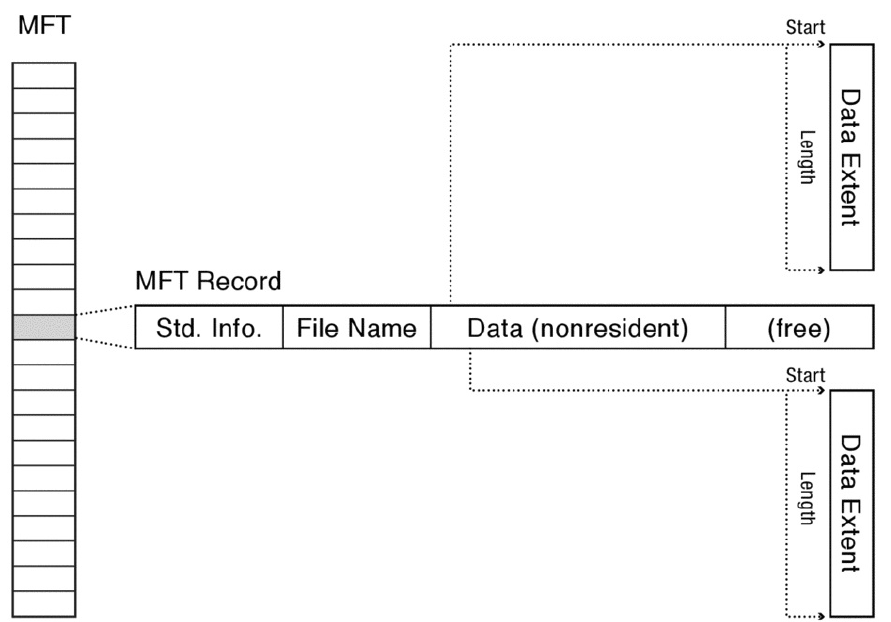
\includegraphics[scale=0.65]{img/fig1308}}
\caption{Estructuras de índices NTFS y datos para un archivo básico con dos extensiones de datos.}
\label{fig1308}
\end{figure}

La \textit{Fig.} \ref{fig1308} ilustra las estructuras de índice para un archivo NTFS básico. Aquí, el registro MFT del archivo incluye un atributo de datos no residente, que es una secuencia de punteros de extensión, cada uno de los cuales especifica el bloque inicial y la longitud en bloques de una extensión de datos. Debido a que las extensiones pueden contener números variables de bloques, incluso un archivo de varios gigabytes puede representarse con uno o varios punteros de extensión en un registro MFT, suponiendo que la fragmentación del sistema de archivos se mantenga bajo control.

Si un archivo es pequeño, se puede usar el atributo de datos para almacenar el contenido real del archivo en su registro MFT como un atributo residente.

Un registro MFT tiene un formato flexible que puede incluir un rango de diferentes atributos. Además de los atributos de datos, hay tres tipos atributos de metadatos comunes, los cuales incluyen:
\begin{itemize}
\item \textbf{Información estándar}. Este atributo contiene información estándar necesaria para todos los archivos. Los campos incluyen las fechas y horas de creación, modificación y último acceso al archivo, el ID del propietario y el especificador de seguridad. También se incluye un conjunto de indicadores que indican información básica como si el archivo es un archivo de sólo lectura, un archivo oculto o un archivo de sistema.
\item \textbf{Nombre del archivo}. Este atributo contiene el nombre del archivo y el número de archivo de su directorio principal. Debido a que un archivo puede tener varios nombres (por ejemplo, si hay varios enlaces físicos al archivo), puede tener varios atributos de nombre de archivo en su registro MFT.
\item \textbf{Lista de atributos}. Dado que los metadatos de un archivo pueden incluir un número variable de atributos de tamaño variable, los metadatos de un archivo pueden ser mayores que un único registro MFT. Cuando se produce este caso, NTFS almacena los atributos en varios registros MFT e incluye una lista de atributos en el primer registro. Cuando está presente, la lista de atributos indica qué atributos se almacenan en los registros MFT.
\end{itemize}

Un archivo puede pasar por cuatro etapas de crecimiento, dependiendo de su tamaño y fragmentación. En primer lugar, un archivo pequeño puede tener su contenido incluido en el registro MFT como un atributo de datos residentes. Segundo, más típicamente, los datos de un archivo se encuentran en un pequeño número de extensiones rastreadas por un solo atributo de datos no residente. En tercer lugar, ocasionalmente, si un archivo es grande y el sistema de archivos fragmentado, un archivo puede tener tantas extensiones que los punteros de extensión no caben en un solo registro MFT. En este caso, como un archivo puede tener múltiples atributos de datos no residentes en múltiples registros MFT, con la lista de atributos en el primer registro MFT que indica qué registros MFT rastrean los rangos de extensiones. Cuarto y finalmente, si un archivo es enorme o la fragmentación del sistema de archivos es extrema, la lista de atributos de un archivo se puede hacer no residente, permitiendo casi arbitrariamente un gran número de registros MFT.

Incluso la tabla de archivos maestra, en sí, se almacena como un archivo, número de archivo 0, llamado \$MFT. Por lo tanto, tenemos que encontrar la primera entrada de la MFT para leer la MFT. Para localizar el MFT, el primer sector de un volumen NTFS incluye un puntero a la primera entrada del MFT. Almacenar el MFT en un archivo evita la necesidad de asignar estáticamente todas las entradas MFT como una matriz fija en una ubicación predeterminada. En su lugar, NTFS comienza con un MFT pequeño y crece a medida que se crean nuevos archivos y se necesitan nuevas entradas.

\textbf{Heurística de localidad}.
La mayoría de las implementaciones de NTFS usan una variación del \textit{mejor ajuste} (best fit), donde el sistema intenta colocar un archivo recientemente asignado en la región libre más pequeña que es lo suficientemente grande como para contenerla. En la variación de NTFS, en lugar de intentar mantener el mapa de bits de asignación para todo el disco en memoria, el sistema almacena en caché el estado de asignación para una región más pequeña del disco y busca primero esa región. Si el caché de mapa de bits contiene información para las áreas donde se han producido las escrituras recientemente, entonces las escrituras que ocurren juntas en el tiempo tienden a agruparse.

Una característica importante de NTFS para optimizar su colocación de mejor ajuste es la interfaz {\mf SetEndOfFile()}, que permite a una aplicación especificar el tamaño esperado de un archivo en el momento de la creación. En contraste, FFS asigna bloques de archivos a medida que se escriben, sin saber cuánto crecerá el archivo.

Para evitar que el archivo de tabla de archivos maestros (\$MFT) se vuelva fragmentado, NTFS reserva parte del inicio del volumen (por ejemplo, el primer 12,5\% del volumen) para la expansión MFT. NTFS no coloca bloques de archivos en el área de reserva MFT hasta que el área no reservada está llena, momento en el que reduce a la mitad el tamaño del área de reserva de MFT y continúa. A medida que el volumen continúa llenando, el NTFS continúa reduciendo a la mitad el área de reserva hasta que alcanza el punto donde el área de reserva restante está más de la mitad llena.

Finalmente, los sistemas operativos de Microsoft con NTFS incluyen una utilidad de desfragmentación que toma archivos fragmentados y los reescribe en regiones contiguas de disco.


%------------------------------------------------------------------------------------------------------------------------------------------
%	BIBLIOGRAFÍA
%------------------------------------------------------------------------------------------------------------------------------------------
\nocite{*}
\bibliographystyle{resumen}
\bibliography{resumen}


\end{document}